\documentclass[]{book}
\usepackage{lmodern}
\usepackage{amssymb,amsmath}
\usepackage{ifxetex,ifluatex}
\usepackage{fixltx2e} % provides \textsubscript
\ifnum 0\ifxetex 1\fi\ifluatex 1\fi=0 % if pdftex
  \usepackage[T1]{fontenc}
  \usepackage[utf8]{inputenc}
\else % if luatex or xelatex
  \ifxetex
    \usepackage{mathspec}
  \else
    \usepackage{fontspec}
  \fi
  \defaultfontfeatures{Ligatures=TeX,Scale=MatchLowercase}
\fi
% use upquote if available, for straight quotes in verbatim environments
\IfFileExists{upquote.sty}{\usepackage{upquote}}{}
% use microtype if available
\IfFileExists{microtype.sty}{%
\usepackage[]{microtype}
\UseMicrotypeSet[protrusion]{basicmath} % disable protrusion for tt fonts
}{}
\PassOptionsToPackage{hyphens}{url} % url is loaded by hyperref
\usepackage[unicode=true]{hyperref}
\hypersetup{
            pdftitle={Applied Missing data analysis with SPSS and R(Studio)},
            pdfauthor={Martijn Heymans and Iris Eekhout},
            pdfborder={0 0 0},
            breaklinks=true}
\urlstyle{same}  % don't use monospace font for urls
\usepackage{natbib}
\bibliographystyle{apalike}
\usepackage{color}
\usepackage{fancyvrb}
\newcommand{\VerbBar}{|}
\newcommand{\VERB}{\Verb[commandchars=\\\{\}]}
\DefineVerbatimEnvironment{Highlighting}{Verbatim}{commandchars=\\\{\}}
% Add ',fontsize=\small' for more characters per line
\usepackage{framed}
\definecolor{shadecolor}{RGB}{248,248,248}
\newenvironment{Shaded}{\begin{snugshade}}{\end{snugshade}}
\newcommand{\KeywordTok}[1]{\textcolor[rgb]{0.13,0.29,0.53}{\textbf{#1}}}
\newcommand{\DataTypeTok}[1]{\textcolor[rgb]{0.13,0.29,0.53}{#1}}
\newcommand{\DecValTok}[1]{\textcolor[rgb]{0.00,0.00,0.81}{#1}}
\newcommand{\BaseNTok}[1]{\textcolor[rgb]{0.00,0.00,0.81}{#1}}
\newcommand{\FloatTok}[1]{\textcolor[rgb]{0.00,0.00,0.81}{#1}}
\newcommand{\ConstantTok}[1]{\textcolor[rgb]{0.00,0.00,0.00}{#1}}
\newcommand{\CharTok}[1]{\textcolor[rgb]{0.31,0.60,0.02}{#1}}
\newcommand{\SpecialCharTok}[1]{\textcolor[rgb]{0.00,0.00,0.00}{#1}}
\newcommand{\StringTok}[1]{\textcolor[rgb]{0.31,0.60,0.02}{#1}}
\newcommand{\VerbatimStringTok}[1]{\textcolor[rgb]{0.31,0.60,0.02}{#1}}
\newcommand{\SpecialStringTok}[1]{\textcolor[rgb]{0.31,0.60,0.02}{#1}}
\newcommand{\ImportTok}[1]{#1}
\newcommand{\CommentTok}[1]{\textcolor[rgb]{0.56,0.35,0.01}{\textit{#1}}}
\newcommand{\DocumentationTok}[1]{\textcolor[rgb]{0.56,0.35,0.01}{\textbf{\textit{#1}}}}
\newcommand{\AnnotationTok}[1]{\textcolor[rgb]{0.56,0.35,0.01}{\textbf{\textit{#1}}}}
\newcommand{\CommentVarTok}[1]{\textcolor[rgb]{0.56,0.35,0.01}{\textbf{\textit{#1}}}}
\newcommand{\OtherTok}[1]{\textcolor[rgb]{0.56,0.35,0.01}{#1}}
\newcommand{\FunctionTok}[1]{\textcolor[rgb]{0.00,0.00,0.00}{#1}}
\newcommand{\VariableTok}[1]{\textcolor[rgb]{0.00,0.00,0.00}{#1}}
\newcommand{\ControlFlowTok}[1]{\textcolor[rgb]{0.13,0.29,0.53}{\textbf{#1}}}
\newcommand{\OperatorTok}[1]{\textcolor[rgb]{0.81,0.36,0.00}{\textbf{#1}}}
\newcommand{\BuiltInTok}[1]{#1}
\newcommand{\ExtensionTok}[1]{#1}
\newcommand{\PreprocessorTok}[1]{\textcolor[rgb]{0.56,0.35,0.01}{\textit{#1}}}
\newcommand{\AttributeTok}[1]{\textcolor[rgb]{0.77,0.63,0.00}{#1}}
\newcommand{\RegionMarkerTok}[1]{#1}
\newcommand{\InformationTok}[1]{\textcolor[rgb]{0.56,0.35,0.01}{\textbf{\textit{#1}}}}
\newcommand{\WarningTok}[1]{\textcolor[rgb]{0.56,0.35,0.01}{\textbf{\textit{#1}}}}
\newcommand{\AlertTok}[1]{\textcolor[rgb]{0.94,0.16,0.16}{#1}}
\newcommand{\ErrorTok}[1]{\textcolor[rgb]{0.64,0.00,0.00}{\textbf{#1}}}
\newcommand{\NormalTok}[1]{#1}
\usepackage{longtable,booktabs}
% Fix footnotes in tables (requires footnote package)
\IfFileExists{footnote.sty}{\usepackage{footnote}\makesavenoteenv{long table}}{}
\usepackage{graphicx,grffile}
\makeatletter
\def\maxwidth{\ifdim\Gin@nat@width>\linewidth\linewidth\else\Gin@nat@width\fi}
\def\maxheight{\ifdim\Gin@nat@height>\textheight\textheight\else\Gin@nat@height\fi}
\makeatother
% Scale images if necessary, so that they will not overflow the page
% margins by default, and it is still possible to overwrite the defaults
% using explicit options in \includegraphics[width, height, ...]{}
\setkeys{Gin}{width=\maxwidth,height=\maxheight,keepaspectratio}
\IfFileExists{parskip.sty}{%
\usepackage{parskip}
}{% else
\setlength{\parindent}{0pt}
\setlength{\parskip}{6pt plus 2pt minus 1pt}
}
\setlength{\emergencystretch}{3em}  % prevent overfull lines
\providecommand{\tightlist}{%
  \setlength{\itemsep}{0pt}\setlength{\parskip}{0pt}}
\setcounter{secnumdepth}{5}
% Redefines (sub)paragraphs to behave more like sections
\ifx\paragraph\undefined\else
\let\oldparagraph\paragraph
\renewcommand{\paragraph}[1]{\oldparagraph{#1}\mbox{}}
\fi
\ifx\subparagraph\undefined\else
\let\oldsubparagraph\subparagraph
\renewcommand{\subparagraph}[1]{\oldsubparagraph{#1}\mbox{}}
\fi

% set default figure placement to htbp
\makeatletter
\def\fps@figure{htbp}
\makeatother

\usepackage{booktabs}

\title{Applied Missing data analysis with SPSS and R(Studio)}
\author{Martijn Heymans and Iris Eekhout}
\date{2018-10-21}

\usepackage{amsthm}
\newtheorem{theorem}{Theorem}[chapter]
\newtheorem{lemma}{Lemma}[chapter]
\theoremstyle{definition}
\newtheorem{definition}{Definition}[chapter]
\newtheorem{corollary}{Corollary}[chapter]
\newtheorem{proposition}{Proposition}[chapter]
\theoremstyle{definition}
\newtheorem{example}{Example}[chapter]
\theoremstyle{definition}
\newtheorem{exercise}{Exercise}[chapter]
\theoremstyle{remark}
\newtheorem*{remark}{Remark}
\newtheorem*{solution}{Solution}
\begin{document}
\maketitle

{
\setcounter{tocdepth}{1}
\tableofcontents
}
\chapter*{Preface}\label{preface}
\addcontentsline{toc}{chapter}{Preface}

The attention for missing data is growing and so will be the application
of methods to solve the missing data problem. From our experience,
researchers with missing data still find it difficult to reserve time to
evaluate the missing data and from that to find a reasonable solution to
handle their missing data for their main data analysis. This manual is
developed for researchers that are looking for a solution of their
missing data problem or want to learn more about missing data. The
manual is developed as a result of a missing data course that we give.
Further, we are also active in providing statistical advice in general
and more specific about missing data. Because our time to give advice is
mostly limited we wanted to give researchers a practical guide to help
them get started with their missing data problem. Leading methodologists
and statisticians and leading journals have published papers about the
problems of missing data and warned researchers to take missing data
seriously (Sterne et al., BMJ 2009, Little et al. NEJM 2012, Peng et al.
2015, JAMA). Hopefully this manual will help researchers to find the
best solution for their missing data problem. We hope you will enjoy
this manual and that you learn from it, at least to take missing data
seriously and that you will use recommended methods to solve your
missing data problem.

\section{The goal of this Manual}\label{the-goal-of-this-manual}

In this manual the software packages SPSS and R play a central role. The
combination of these two software packages may seem a coincidence, but
it is not. For a long time, SPSS was the most popular software package
worldwide to do statistical data analysis. Currently, R is growing in
popularity fast and will probably become one of the most popular
Software packages to do data analysis. Also for applied researchers.
Both SPSS and R have their advantages and disadvantages. An advantage of
SPSS is that it is a user-friendly software package compared to R and
works with windows where you can for example drag your variables to.
Subsequently, you can click the OK button and the statistical analysis
procedure you prespecified gives you the output results. A disadvantage
of SPSS may be that you are overloaded with statistical output that may
not all needed to answer your research question. Compared to SPSS you
could say that R is a more user-unfriendly software package where you
need to use R code to activate statistical procedures and to get
statistical results. R output will show more specific results, without
extra information. Furthermore, R works much faster when it comes to
running statistical procedures by using 1 or 2 lines of R code, compared
to visiting a couple of windows in SPSS to activate the same statistical
test. There is one other advantage of R and that is, that it is open
source. This makes it possible for applied researchers to follow the
calculations of complex procedures as the estimation of missing values
closely along the line. You could say that R brings you to the heart of
the matter. With R it is possible to turn complex data analysis
functions and formula´s into computer code that can be used by everybody
and vice versa. Because it is open source, you are able to read the code
that is used for the analysis and to relate that code or pieces of code
to the statistical output. This makes it possible to evaluate step by
step the code and thus the statistical procedures and relate them to the
subsequent results. You can copy specific parts of code from functions
that others have written and evaluate what happens. This is one of the
major advantages of R if you compare it to the closed source statistical
package SPSS. R brings you a big learning environment when it comes to
the understanding of all kind of statistical procedures as missing data
analysis.

\section{Multiple Imputation in SPSS and
R}\label{multiple-imputation-in-spss-and-r}

Multiple Imputation (MI) is a procedure that is developed in the 1970's
by Donald Rubin. Later, around the 1990´s Multiple imputation was
further developed and became more popular. For a long time, MI was only
available for S-Plus and R software (S-plus is the commercial
alternative of R), where it was further developed by Stef van Buuren, a
statistician from TNO, Leiden, The Netherlands. For a long time, it was
not possible to do MI analysis in SPSS because it was not available in
SPSS. So, it was far out of reach for applied researchers for a long
time. It became available from SPSS version 17. From that time MI is now
used more by applied researchers. In this manual the handling of missing
data is the main topic. We will also show how to apply these methods in
both software packages SPSS and R. To apply the imputation methods that
are discussed both software packages make use of random starting
procedures. SPSS and R use for that intern random number generators.
Because these are different, result might slightly differ. Our intention
is not to compare the software packages SPSS and R and their output
resultys. Both are trustful packages, it is more the estimation
procedures that might lead to the differences. The imputation methods,
will be applied in SPSS version 24 and with R software version 3.4.3.
The R examples will be presented by using the output from RStudio
version (version 1.1.383 -- © 2009-2017 RStudio, Inc.). RStudio is an
integrated development environment (IDE) for R. RStudio includes a wide
range of productivity enhancing features and runs on all major
platforms. As already stated, R allows you to program the statistical
formula's yourself. We have therefore chosen to explain the formula's in
more detail in combination with the application in R. The more applied
researchers will be satisfied with the explanation and application of
methods in SPSS.

\section{Notation and annotation in this
manual}\label{notation-and-annotation-in-this-manual}

The name of R packages, libraries and functions can be recognized by
using Courier new lettertype, for example the package mice will be
written as mice.

R code of the procedures used in the manual is marked grey and the
explanation in these grey parts can be found in the grey parts itself
annotated by the \# symbol. The lines that start with the symbol
\textgreater{} are R Code lines that have been running in the R Console
in RStudio. Example:

\textbf{R code XX}

\begin{Shaded}
\begin{Highlighting}[]
\CommentTok{# Activate the foreign package and read in the SPSS dataset}

\KeywordTok{library}\NormalTok{(foreign)}
\NormalTok{dataset <-}\StringTok{ }\KeywordTok{read.spss}\NormalTok{(}\DataTypeTok{file=}\StringTok{"data/Backpain 50 missing.sav"}\NormalTok{, }\DataTypeTok{to.data.frame=}\NormalTok{T)}
\end{Highlighting}
\end{Shaded}

\begin{verbatim}
## re-encoding from UTF-8
\end{verbatim}

\chapter{Software applications}\label{software-applications}

We start the book with an introduction into the software packages SPSS
and RStudio that are needed to conduct the procedures explained in the
other chapters. If you are an user of SPSS or RStudio you can skip this
Chapter without losing relevant information and continue with the next
chapter.

\section{SPSS, Data and Variable View
windows}\label{spss-data-and-variable-view-windows}

In this book we work with SPSS version 24 (IBM, 2016). When you open
SPSS you see an empty Data View window, you are than in the SPSS Data
Editor window. This window is always open when you start SPSS.

In the SPSS Data Editor, you have the possibility to go to the Data View
and Variable View windows. In the Data View window, you can enter data
yourself or read in data by using the options in the file menu. In
(Figure \ref{fig:fig2}) you see an example of a dataset in the Data View
window. Each row in the Data View window represents a case and in the
columns you find the variable names. In the Data View window, you can
start all kind of data manipulations by using the different menu's above
in the window.

\begin{figure}

{\centering 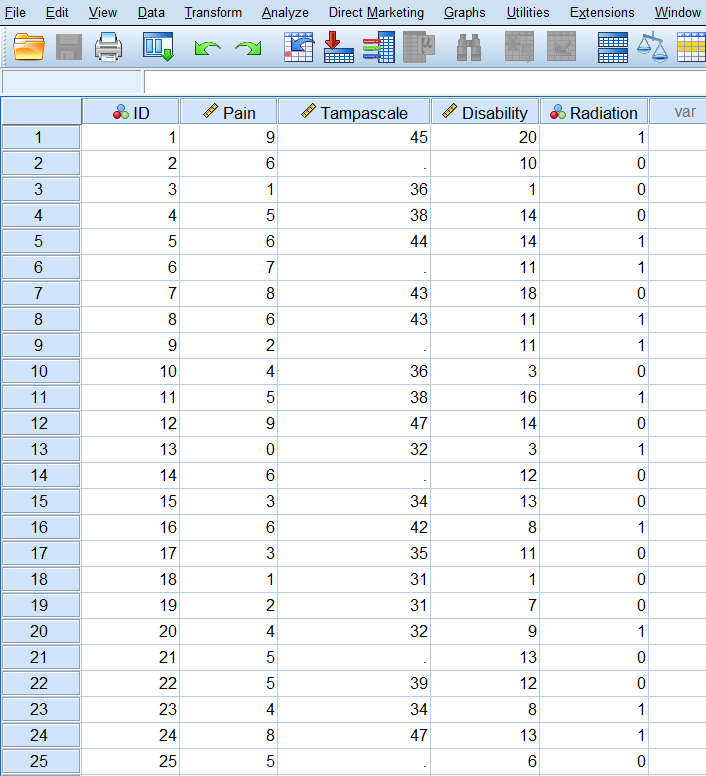
\includegraphics[width=0.9\linewidth]{images/fig1.2} 

}

\caption{Data View window in SPSS}\label{fig:fig2}
\end{figure}

In the lower left corner of the window you can click on the tab Variable
View and the Variable view window will appear (Figure \ref{fig:fig3}).

\begin{figure}

{\centering 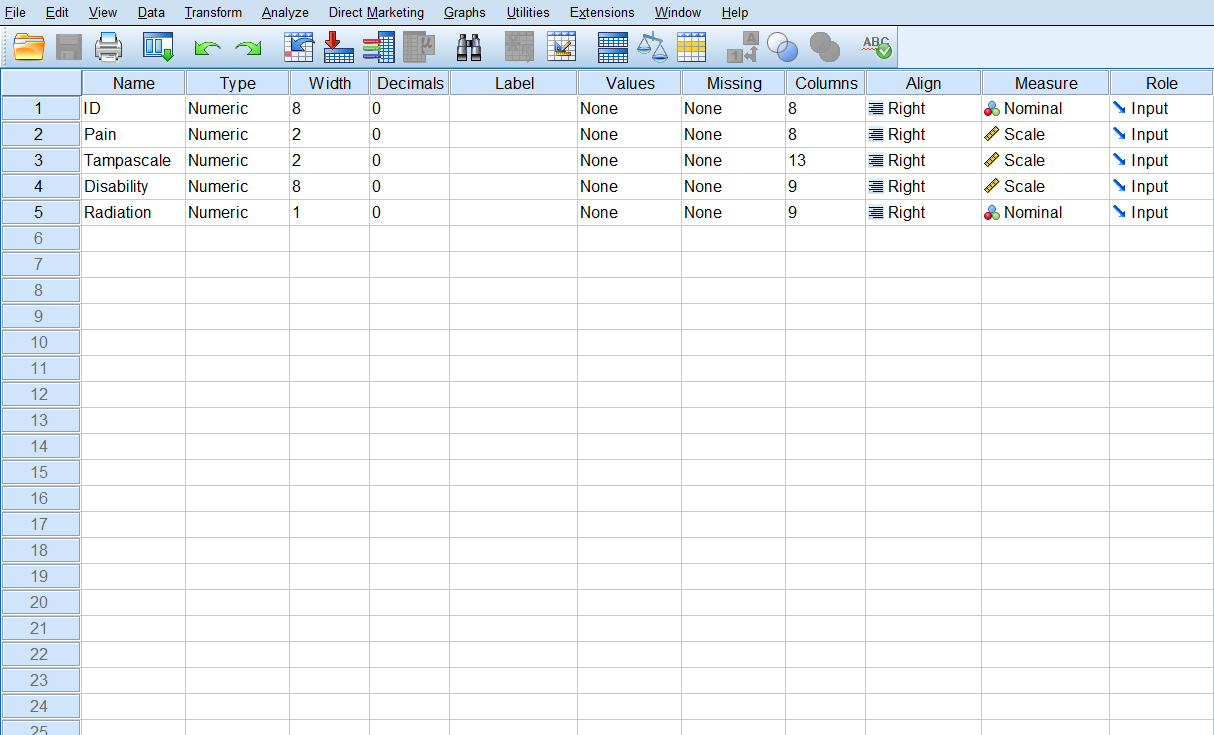
\includegraphics[width=0.9\linewidth]{images/fig1.3} 

}

\caption{Variable View window in SPSS}\label{fig:fig3}
\end{figure}

In the Variable View window, you can add new variables, by entering the
name in the name column. Further, you can change the columns by using
the options: Type: i.g. numeric or string; Width: number of digits;
Decimals: the number of decimal places displayed; Label: The variable
name; Values: To assign numbers to the categories of a variable;
Missing: you can define specified data values as user-missing or system
missing; Columns: To change the number of characters displayed in the
Data View window; Align: to specify the alignment of the data; Measure:
to specify the level of each variable, scale (continuous), ordinal or
nominal; Role: Here you can define the role of the variable during your
analysis. Examples are, Input for independent variable, Target for
dependent or outcome variable, Both, independent and dependent variable.
There are more possibilities, but most of the times you use the default
Input setting.

\section{Analyzing data in SPSS}\label{analyzing-data-in-spss}

All statistical procedures in SPSS can be found under the Analyze button
(Figure \ref{fig:fig4}). Here you also find the option ``Multiple
Imputation'' which plays an important role in this manual.

\begin{figure}

{\centering 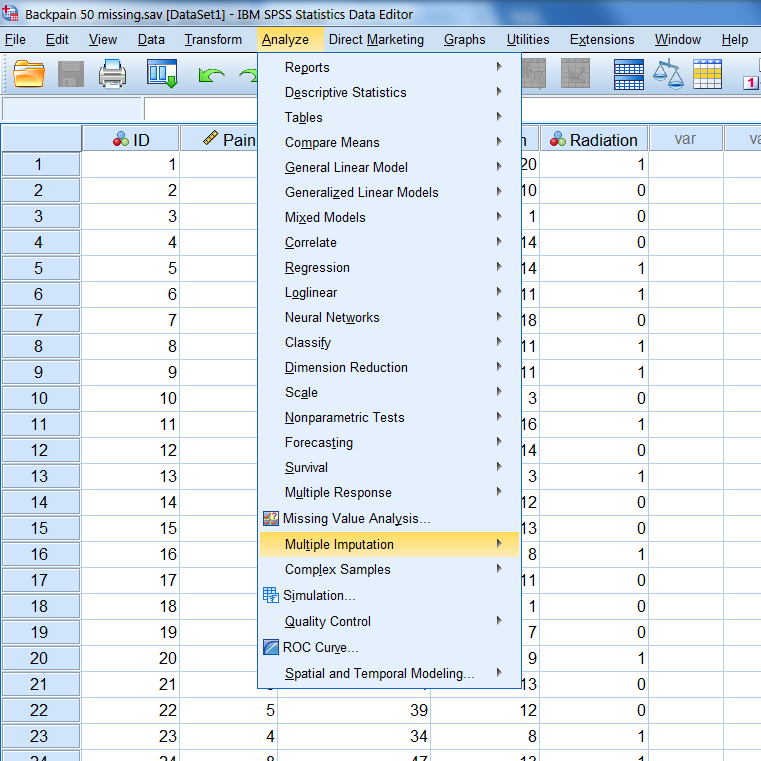
\includegraphics[width=0.9\linewidth]{images/fig1.4} 

}

\caption{Statistical procedures that can be found under the Analyze menu in SPSS}\label{fig:fig4}
\end{figure}

\section{The Output window in SPSS}\label{the-output-window-in-spss}

If you have run your analyses in SPSS, an SPSS Output (or viewer) Window
will pop-up. The main body of the Output Window consists of two panes
(left and right panes). In the left pane you will find an outline of the
output. In the right pane you will find the actual output of your
statistical procedure (Figure \ref{fig:fig5}).

\begin{figure}

{\centering 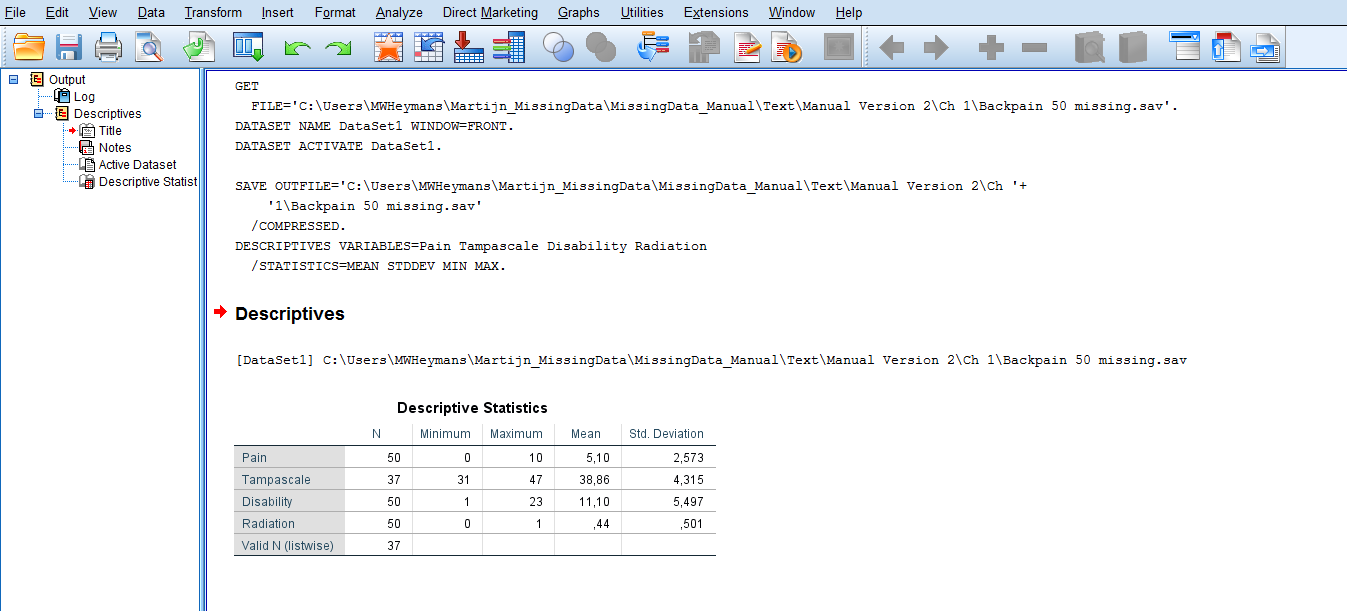
\includegraphics[width=0.9\linewidth]{images/fig1.5} 

}

\caption{Part of the Output or Viewer window in SPSS after making use of Descriptive Statistics under the Analyze menu}\label{fig:fig5}
\end{figure}

\section{The Syntax Editor in SPSS}\label{the-syntax-editor-in-spss}

In the syntax editor of SPSS, you use the SPSS syntax programming
language. You can run all SPSS procedures by typing in commands in this
syntax editor window, instead of using the graphical user interface,
i.e.~by using your mouse and clicking on the menu´s. You can get access
to the syntax window in two ways. The first is just by opening a new
syntax file by navigating to

\begin{quote}
File -\textgreater{} New -\textgreater{} Syntax.
\end{quote}

This will open a new syntax window (Figure \ref{fig:fig6}).

\begin{figure}

{\centering 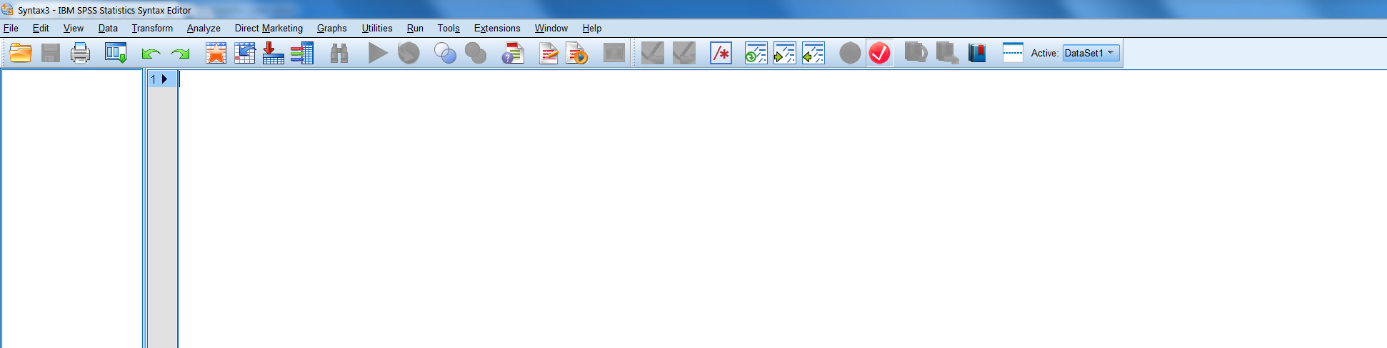
\includegraphics[width=0.9\linewidth]{images/fig1.6} 

}

\caption{Screenshot of new syntax file}\label{fig:fig6}
\end{figure}

You can also generate syntax by accessing statistical procedures through
the dropdown menus and clicking the \texttt{Paste} button instead of
clicking the OK button after you have specified the options. Than a new
Syntax Editor window will pop up or the new syntax will automatically be
added to the open Syntax Editor window. An example can be found in
Figure \ref{fig:fig7}, where the syntax is shown for the Descriptive
Statistics procedure of Figure \ref{fig:fig5}.

\begin{figure}

{\centering 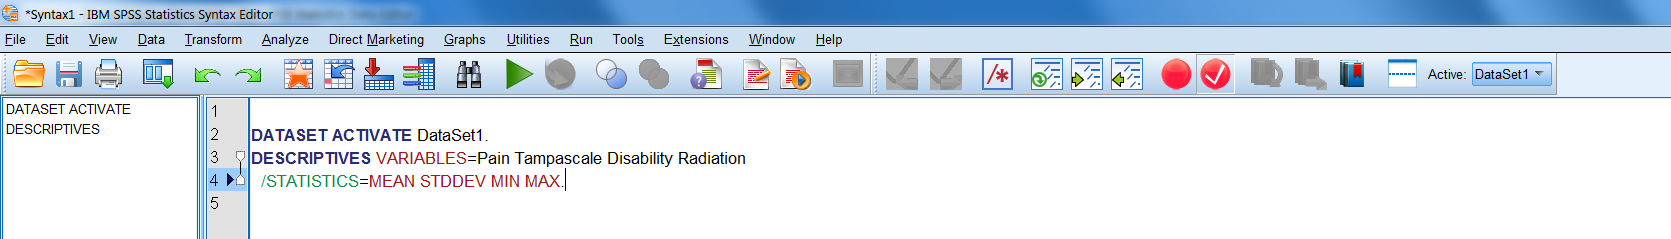
\includegraphics[width=0.9\linewidth]{images/fig1.7} 

}

\caption{Screenshot of Syntax editor of SPSS including the Syntax code for descriptive statisitcs}\label{fig:fig7}
\end{figure}

In this manual we will not use SPSS syntax code to access statistical
procedures. SPSS is most frequently used via the graphical user
interface, and we will use that method also in this manual.

\section{Reading and saving data in
SPSS}\label{reading-and-saving-data-in-spss}

You can Read data in, in SPSS via the menu File:

\begin{quote}
File -\textgreater{} Open -\textgreater{} Data.
\end{quote}

All kind of file types can be selected. Of course the SPSS .sav files,
but also .por, .xlsx, .cvs, SAS, Stata, etc. (Figure 1.8). After you
have selected a specific file type other than SPSS you may have to go
through several steps before you see the data in the Data View window.
These steps are not necessary for SPSS files, they open directly in the
data editor.

\begin{figure}

{\centering 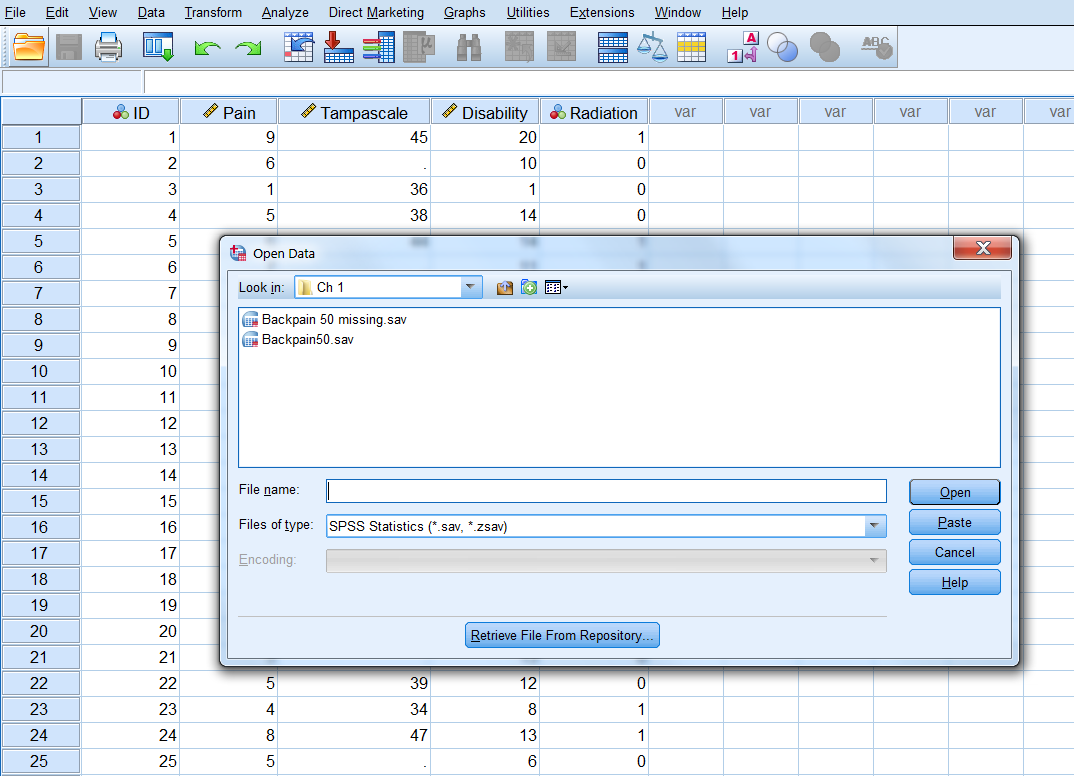
\includegraphics[width=0.9\linewidth]{images/fig1.8} 

}

\caption{Window to read in different file types in SPSS}\label{fig:fig8}
\end{figure}

Saving files in SPSS is possible via the Save Data As option under the
menu File. You can choose the same kind of file types (Figure
\ref{fig:fig9}).

\section{R and RStudio}\label{r-and-rstudio}

RStudio is an integrated environment to work with the software program
R. Consequently, to work with RStudio, R has to be installed. RStudio
uses the R language and is also freely available. In this manual we will
only show some possibilities and options in RStudio that are needed to
run the R code and the programs that are discussed in this manual. For
more information about RStudio and its possibilities visit the RStudio
website at www.rstudio.com. When you open RStudio the following screen
will appear.

\begin{figure}

{\centering 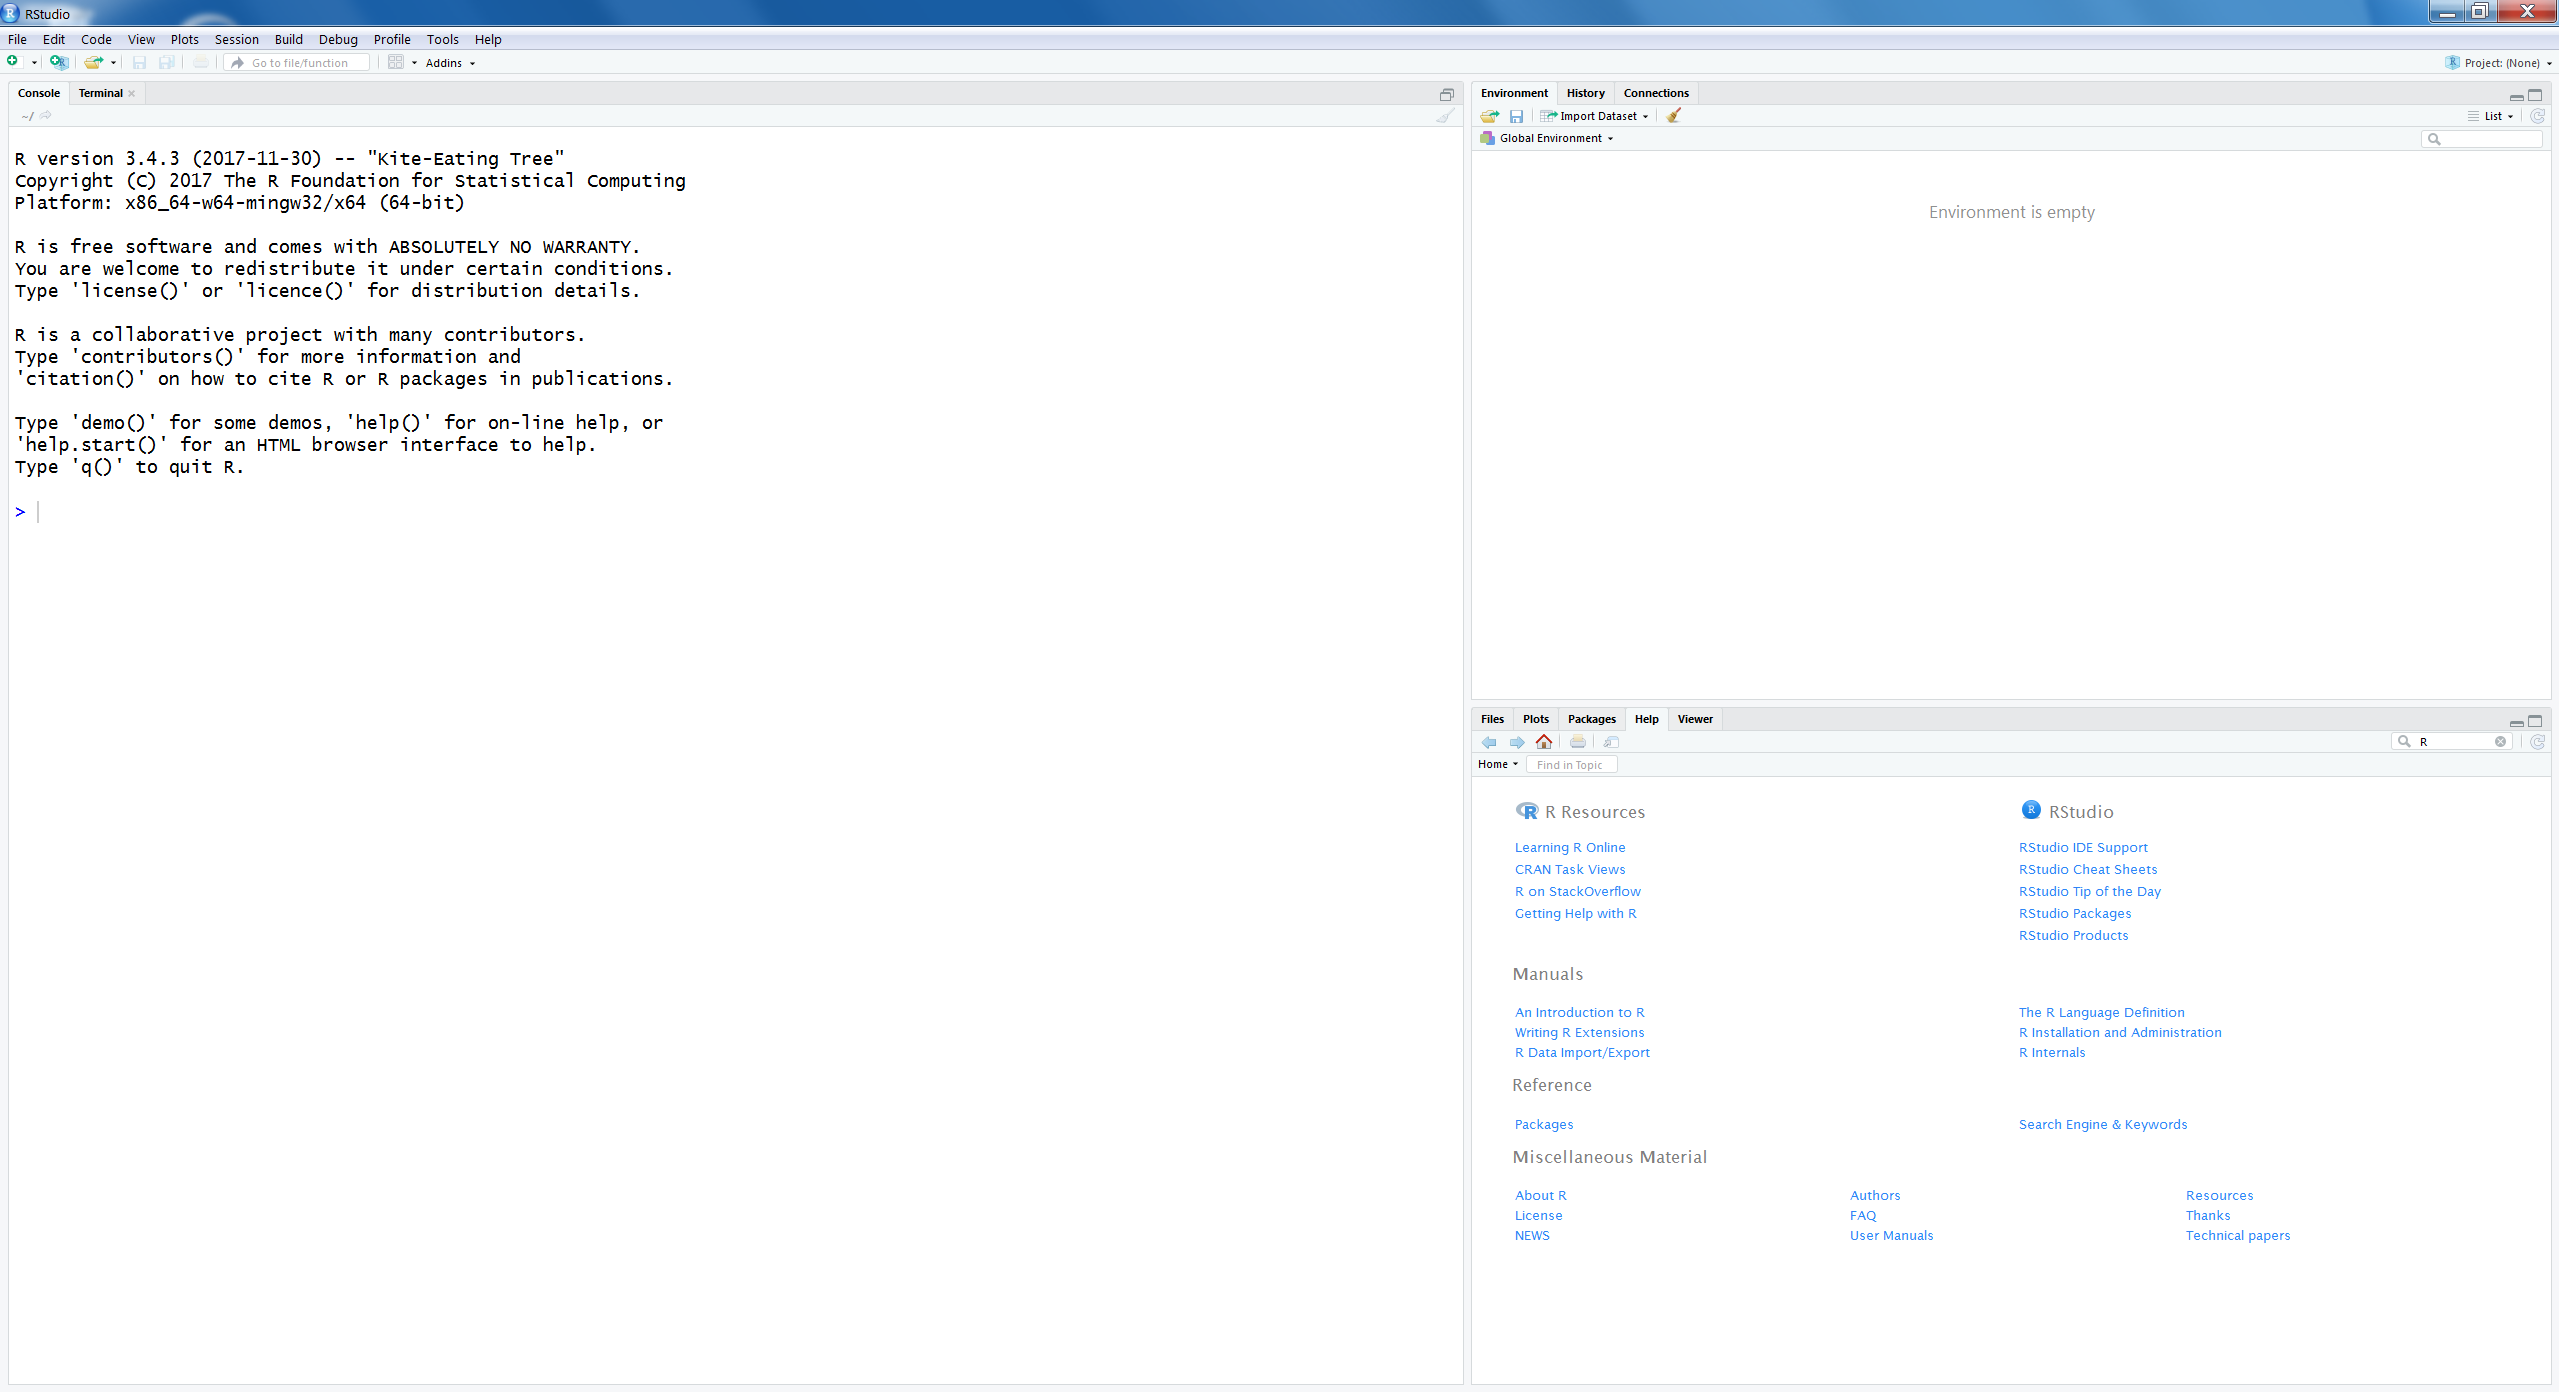
\includegraphics[width=0.9\linewidth]{images/fig1.10} 

}

\caption{First screen that appears after you have started RStudio}\label{fig:fig10}
\end{figure}

There are three windows opened:

\begin{enumerate}
\def\labelenumi{\arabic{enumi}.}
\tightlist
\item
  On the left is the Console window
\end{enumerate}

This is the main window to run R code (see below for more information
about the Console window).

\begin{enumerate}
\def\labelenumi{\arabic{enumi}.}
\setcounter{enumi}{1}
\item
  Right above is the window where you can choose between the Environment
  and History tabs (e.g.~history tracks the code you typed in the
  Console window).
\item
  At the right site below is the window where you can choose between
  Files, Plots, Packages, Help and Viewer tabs.
\end{enumerate}

\subsection{The role of the Console
Window}\label{the-role-of-the-console-window}

When you enter code in the Console window you will directly receive a
result. For example, when you type \texttt{3\ +\ 3} the result will
appear directly.

\begin{Shaded}
\begin{Highlighting}[]
\DecValTok{3} \OperatorTok{+}\StringTok{ }\DecValTok{3}
\end{Highlighting}
\end{Shaded}

\begin{verbatim}
## [1] 6
\end{verbatim}

Other multiplication procedures as divide, square, etc. can also be
executed. The main use for R is its functions. For example, to generate
20 random numbers you use the following function code (we will discuss
more about functions in R later):

\begin{Shaded}
\begin{Highlighting}[]
\KeywordTok{rnorm}\NormalTok{(}\DecValTok{20}\NormalTok{)}
\end{Highlighting}
\end{Shaded}

\begin{verbatim}
##  [1] -1.7837970  1.8680008  0.4986246 -2.8537612  2.5696148 -0.4905977
##  [7] -1.3530066  0.2784674  3.4362621  0.9665584  0.1917680  0.2153195
## [13] -0.4293876  0.2079086 -1.8858143 -0.1891847  2.7196848  0.4403796
## [19] -1.6495320 -0.3074956
\end{verbatim}

The number {[}1{]} between brackets is the index of the first number or
item in the vector.

\subsection{R assignments and objects}\label{r-assignments-and-objects}

In R it is possible to create objects and to assign values to these
objects. In this way it is possible to store some intermediate results
and recall or use them later on. Assigning values to objects is done by
using the assignment operator \texttt{\textless{}-} . You can also use
the = sign as an assignment operator. This is not recommended because
this is also a symbol used for some mathematical operations. For
example, when we want to assign the value 3 to the object x, we use the
following code.

\begin{Shaded}
\begin{Highlighting}[]
\NormalTok{x <-}\StringTok{ }\DecValTok{3} 
\end{Highlighting}
\end{Shaded}

When we subsequently type in the letter x we get the following result:

\begin{Shaded}
\begin{Highlighting}[]
\NormalTok{x }
\end{Highlighting}
\end{Shaded}

\begin{verbatim}
## [1] 3
\end{verbatim}

As result we see the value 3 again. Now the value 3 is assigned to the
object x. In R all kind of information can be assigned to an object,
i.e.~one number, a vector of numbers, results from analysis or other R
objects such as data frames, matrices or lists. Objects can have all
kinds of different names, composed of different letters and numbers.
Here are some examples where number 3 is assigned to different objects
with different names:

\begin{Shaded}
\begin{Highlighting}[]
\NormalTok{test <-}\StringTok{ }\DecValTok{3}
\NormalTok{test.}\DecValTok{1}\NormalTok{ <-}\StringTok{ }\DecValTok{3}
\NormalTok{test.manual <-}\StringTok{ }\DecValTok{3}
\NormalTok{test}
\end{Highlighting}
\end{Shaded}

\begin{verbatim}
## [1] 3
\end{verbatim}

\begin{Shaded}
\begin{Highlighting}[]
\NormalTok{test.}\DecValTok{1}
\end{Highlighting}
\end{Shaded}

\begin{verbatim}
## [1] 3
\end{verbatim}

\begin{Shaded}
\begin{Highlighting}[]
\NormalTok{test.manual }
\end{Highlighting}
\end{Shaded}

\begin{verbatim}
## [1] 3
\end{verbatim}

Note that some letters and words are used by R itself. It is not
recommended to use these leters as names for objects in R that you
create yourself. For example, the letter T and F are used as TRUE and
FALSE by R. Other letters that are already in use are c, q, t, C, D, I
and diff, df, and pt.

\subsection{Vectors, matrices, lists and data
frames}\label{vectors-matrices-lists-and-data-frames}

\emph{Vectors} In the previous paragraph we created the one-vector x,
i.e.~a vector that contained only one number, the number 3. Mostly you
do your analysis on more numbers than just one. R has several
possibilities to create objects with more data. We start with a simple
dataset, called a data vector, which is an array of numbers (such as
created in R code 1.2. A vector can be created by the following code:

\begin{Shaded}
\begin{Highlighting}[]
\NormalTok{y <-}\StringTok{ }\KeywordTok{c}\NormalTok{(}\DecValTok{1}\NormalTok{, }\DecValTok{2}\NormalTok{, }\DecValTok{3}\NormalTok{, }\DecValTok{4}\NormalTok{, }\DecValTok{5}\NormalTok{)}
\NormalTok{y}
\end{Highlighting}
\end{Shaded}

\begin{verbatim}
## [1] 1 2 3 4 5
\end{verbatim}

Now the numbers 1, 2, 3, 4 and 5 are assigned to the data vector y. The
``c'' in the above code stand for concatenate which makes that all
separate (one-vector) numbers are merged into one vector. It is also
possible to create character vectors, which are vectors that contain
strings (text). An example:

\begin{Shaded}
\begin{Highlighting}[]
\NormalTok{y <-}\StringTok{ }\KeywordTok{c}\NormalTok{(}\StringTok{"a"}\NormalTok{, }\StringTok{"b"}\NormalTok{, }\StringTok{"test"}\NormalTok{)}
\NormalTok{y}
\end{Highlighting}
\end{Shaded}

\begin{verbatim}
## [1] "a"    "b"    "test"
\end{verbatim}

Vectors can also be made by using the ``:'' symbol. With that symbol it
is easy to generate a sequence of numbers. An example:

\begin{Shaded}
\begin{Highlighting}[]
\NormalTok{y <-}\StringTok{ }\DecValTok{1}\OperatorTok{:}\DecValTok{10}
\NormalTok{y}
\end{Highlighting}
\end{Shaded}

\begin{verbatim}
##  [1]  1  2  3  4  5  6  7  8  9 10
\end{verbatim}

\begin{Shaded}
\begin{Highlighting}[]
\NormalTok{y <-}\StringTok{ }\DecValTok{2}\OperatorTok{:}\DecValTok{6}
\NormalTok{y}
\end{Highlighting}
\end{Shaded}

\begin{verbatim}
## [1] 2 3 4 5 6
\end{verbatim}

Both lines of code produce a vector containing a sequence of numbers.
The first example produces the numbers 1 to 10 and the second example
the numbers 2 to 6.

\emph{Matrix} A matrix in R contains rows and columns and can be created
by using the matrix function.

\begin{Shaded}
\begin{Highlighting}[]
\KeywordTok{matrix}\NormalTok{(}\KeywordTok{c}\NormalTok{(}\DecValTok{1}\NormalTok{, }\DecValTok{2}\NormalTok{, }\DecValTok{3}\NormalTok{, }\DecValTok{4}\NormalTok{, }\DecValTok{5}\NormalTok{, }\DecValTok{6}\NormalTok{), }\DataTypeTok{nrow=}\DecValTok{2}\NormalTok{, }\DataTypeTok{ncol=}\DecValTok{3}\NormalTok{)}
\end{Highlighting}
\end{Shaded}

\begin{verbatim}
##      [,1] [,2] [,3]
## [1,]    1    3    5
## [2,]    2    4    6
\end{verbatim}

Now we have created a matrix with 2 rows and 3 columns. In essence we
converted the vector c(1, 2, 3, 4, 5, 6) into a matrix.

\emph{List} Another popular R object class is a list. The advantage of a
list is that it can contain components of different formats. Let's look
at an example using the following code:

\begin{Shaded}
\begin{Highlighting}[]
\NormalTok{x <-}\StringTok{ }\DecValTok{1}\OperatorTok{:}\DecValTok{5}
\NormalTok{x}
\end{Highlighting}
\end{Shaded}

\begin{verbatim}
## [1] 1 2 3 4 5
\end{verbatim}

\begin{Shaded}
\begin{Highlighting}[]
\NormalTok{y <-}\StringTok{ }\KeywordTok{c}\NormalTok{(}\StringTok{"a"}\NormalTok{, }\StringTok{"b"}\NormalTok{, }\StringTok{"test"}\NormalTok{)}
\NormalTok{z <-}\StringTok{ }\KeywordTok{list}\NormalTok{(}\DataTypeTok{x=}\NormalTok{x, }\DataTypeTok{y=}\NormalTok{y)}
\NormalTok{z}
\end{Highlighting}
\end{Shaded}

\begin{verbatim}
## $x
## [1] 1 2 3 4 5
## 
## $y
## [1] "a"    "b"    "test"
\end{verbatim}

The code created the list object z consisting of the two components x
and y which are the vectors that were created above. You can see that in
a list two components of different data type can be combined, a numeric
and a character factor. The names of the list components are indicated
by the dollar sign,
\(. The list component can be obtained separately by typing z\)x for
component x or x\$y for component y.

\emph{Dataframe} Mostly we work with datasets that contain information
of different variables and persons. In R such a dataset is called a
dataframe. In essence, a dataframe in R is a list, where each component
of the list is a vector of equal length. This example code first creates
a list, consisting of 3 vectors of the same length. Than this list is
converted into a dataframe, using the data.frame function.

\begin{Shaded}
\begin{Highlighting}[]
\NormalTok{k <-}\StringTok{ }\KeywordTok{list}\NormalTok{(}\DataTypeTok{a=}\DecValTok{1}\OperatorTok{:}\DecValTok{10}\NormalTok{, }\DataTypeTok{b=}\DecValTok{11}\OperatorTok{:}\DecValTok{20}\NormalTok{, }\DataTypeTok{c=}\DecValTok{21}\OperatorTok{:}\DecValTok{30}\NormalTok{)}
\NormalTok{k}
\end{Highlighting}
\end{Shaded}

\begin{verbatim}
## $a
##  [1]  1  2  3  4  5  6  7  8  9 10
## 
## $b
##  [1] 11 12 13 14 15 16 17 18 19 20
## 
## $c
##  [1] 21 22 23 24 25 26 27 28 29 30
\end{verbatim}

\begin{Shaded}
\begin{Highlighting}[]
\NormalTok{z <-}\StringTok{ }\KeywordTok{data.frame}\NormalTok{(k)}
\NormalTok{z}
\end{Highlighting}
\end{Shaded}

\begin{verbatim}
##     a  b  c
## 1   1 11 21
## 2   2 12 22
## 3   3 13 23
## 4   4 14 24
## 5   5 15 25
## 6   6 16 26
## 7   7 17 27
## 8   8 18 28
## 9   9 19 29
## 10 10 20 30
\end{verbatim}

Typically, a dataframe is created by reading in an existing dataset. How
to create a dataframe by reading in a dataset will be further discussed
in the paragraph ``Reading in and saving data''.

\subsection{Indexing Vectors, Matrices, Lists and Data
frames}\label{indexing-vectors-matrices-lists-and-data-frames}

\emph{Vectors} An important operation in R is to select a subset of a
given vector. This is called indexing vectors. This subset of the vector
elements can be assigned to another vector. An example how to do this:

\begin{Shaded}
\begin{Highlighting}[]
\NormalTok{y <-}\StringTok{ }\KeywordTok{c}\NormalTok{(}\DecValTok{3}\NormalTok{, }\DecValTok{5}\NormalTok{, }\DecValTok{2}\NormalTok{, }\DecValTok{8}\NormalTok{, }\DecValTok{5}\NormalTok{, }\DecValTok{4}\NormalTok{, }\DecValTok{8}\NormalTok{, }\DecValTok{1}\NormalTok{, }\DecValTok{3}\NormalTok{, }\DecValTok{6}\NormalTok{)}
\NormalTok{y[}\KeywordTok{c}\NormalTok{(}\DecValTok{1}\NormalTok{, }\DecValTok{4}\NormalTok{)]}
\end{Highlighting}
\end{Shaded}

\begin{verbatim}
## [1] 3 8
\end{verbatim}

The R code y{[}c(1, 4){]}, extracts the first and fourth element of the
vector. Another example is by using the ``:'' symbol, to extract several
subsequent elements:

\begin{Shaded}
\begin{Highlighting}[]
\NormalTok{y[}\DecValTok{2}\OperatorTok{:}\DecValTok{5}\NormalTok{]}
\end{Highlighting}
\end{Shaded}

\begin{verbatim}
## [1] 5 2 8 5
\end{verbatim}

The R code y{[}2:5{]}, extracts the second to the fifth element of the
vector.

A minus sign excludes the specific element from the vector, like:

\begin{Shaded}
\begin{Highlighting}[]
\NormalTok{y[}\OperatorTok{-}\DecValTok{3}\NormalTok{]}
\end{Highlighting}
\end{Shaded}

\begin{verbatim}
## [1] 3 5 8 5 4 8 1 3 6
\end{verbatim}

The R code y{[}-3{]}, excludes the third element of the vector (i.e.~2).
A new vector z can be created where the third and fourth element of the
y vector are excluded, by using the following code:

\begin{Shaded}
\begin{Highlighting}[]
\NormalTok{z <-}\StringTok{ }\NormalTok{y[}\OperatorTok{-}\KeywordTok{c}\NormalTok{(}\DecValTok{3}\NormalTok{, }\DecValTok{4}\NormalTok{)]}
\NormalTok{z}
\end{Highlighting}
\end{Shaded}

\begin{verbatim}
## [1] 3 5 5 4 8 1 3 6
\end{verbatim}

\emph{Matrices} When we index matrices we can choose to index rows,
columns or both. Here are some examples:

First we construct the matrix

\begin{Shaded}
\begin{Highlighting}[]
\NormalTok{z <-}\StringTok{ }\KeywordTok{matrix}\NormalTok{(}\DecValTok{1}\OperatorTok{:}\DecValTok{9}\NormalTok{, }\DataTypeTok{nrow=}\DecValTok{3}\NormalTok{)}
\NormalTok{z}
\end{Highlighting}
\end{Shaded}

\begin{verbatim}
##      [,1] [,2] [,3]
## [1,]    1    4    7
## [2,]    2    5    8
## [3,]    3    6    9
\end{verbatim}

We extract from the first row the number in the second column

\begin{Shaded}
\begin{Highlighting}[]
\NormalTok{z[}\DecValTok{1}\NormalTok{, }\DecValTok{2}\NormalTok{]}
\end{Highlighting}
\end{Shaded}

\begin{verbatim}
## [1] 4
\end{verbatim}

We extract all numbers in each column in the first row

\begin{Shaded}
\begin{Highlighting}[]
\NormalTok{z[}\DecValTok{1}\NormalTok{, ]}
\end{Highlighting}
\end{Shaded}

\begin{verbatim}
## [1] 1 4 7
\end{verbatim}

We extract all numbers in each row of the first column

\begin{Shaded}
\begin{Highlighting}[]
\NormalTok{z[, }\DecValTok{1}\NormalTok{]}
\end{Highlighting}
\end{Shaded}

\begin{verbatim}
## [1] 1 2 3
\end{verbatim}

A minus sign can also be used to delete specific elements or complete
rows or columns.

Omit the first row from the matrix

\begin{Shaded}
\begin{Highlighting}[]
\NormalTok{z[}\OperatorTok{-}\DecValTok{1}\NormalTok{, ]}
\end{Highlighting}
\end{Shaded}

\begin{verbatim}
##      [,1] [,2] [,3]
## [1,]    2    5    8
## [2,]    3    6    9
\end{verbatim}

\emph{Lists} We first create a list with 3 components, each component
consists of a vector of the same length and with 10 elements each.

\begin{Shaded}
\begin{Highlighting}[]
\NormalTok{k <-}\StringTok{ }\KeywordTok{list}\NormalTok{(}\DataTypeTok{a=}\DecValTok{1}\OperatorTok{:}\DecValTok{10}\NormalTok{, }\DataTypeTok{b=}\DecValTok{11}\OperatorTok{:}\DecValTok{20}\NormalTok{, }\DataTypeTok{c=}\DecValTok{21}\OperatorTok{:}\DecValTok{30}\NormalTok{)}
\NormalTok{k}
\end{Highlighting}
\end{Shaded}

\begin{verbatim}
## $a
##  [1]  1  2  3  4  5  6  7  8  9 10
## 
## $b
##  [1] 11 12 13 14 15 16 17 18 19 20
## 
## $c
##  [1] 21 22 23 24 25 26 27 28 29 30
\end{verbatim}

There are several options to index list components and elements of the
components. If we want to index the individual component b we can use
the following code:

\begin{Shaded}
\begin{Highlighting}[]
\NormalTok{k}\OperatorTok{$}\NormalTok{b}
\end{Highlighting}
\end{Shaded}

\begin{verbatim}
##  [1] 11 12 13 14 15 16 17 18 19 20
\end{verbatim}

\begin{Shaded}
\begin{Highlighting}[]
\NormalTok{k[[}\StringTok{"b"}\NormalTok{]]}
\end{Highlighting}
\end{Shaded}

\begin{verbatim}
##  [1] 11 12 13 14 15 16 17 18 19 20
\end{verbatim}

\begin{Shaded}
\begin{Highlighting}[]
\NormalTok{k[[}\DecValTok{2}\NormalTok{]]}
\end{Highlighting}
\end{Shaded}

\begin{verbatim}
##  [1] 11 12 13 14 15 16 17 18 19 20
\end{verbatim}

As you have may noticed, to extract individual list components double
square brackets are used, compared to single brackets for indexing
vectors and matrices.

When we use single brackets, we get the following results:

\begin{Shaded}
\begin{Highlighting}[]
\NormalTok{k[}\StringTok{"b"}\NormalTok{]}
\end{Highlighting}
\end{Shaded}

\begin{verbatim}
## $b
##  [1] 11 12 13 14 15 16 17 18 19 20
\end{verbatim}

The difference between using single and double brackets is that single
brackets return the component data type, which is in this case a vector
(but could be any kind of data type) and single brackets always return a
list.

\emph{Data frames} Indexing data frames follows the same method as
indexing matrices, but we can also use the method that is used to index
lists, since data frames are essentially lists of vectors of the same
length. Data frames consist of rows and columns which can be accessed
separately or both to extract specific elements. We use the data frame
that was constructed in R code 1.11.

\begin{Shaded}
\begin{Highlighting}[]
\NormalTok{z}
\end{Highlighting}
\end{Shaded}

\begin{verbatim}
##      [,1] [,2] [,3]
## [1,]    1    4    7
## [2,]    2    5    8
## [3,]    3    6    9
\end{verbatim}

Examples of indexing the first column are:

\begin{Shaded}
\begin{Highlighting}[]
\NormalTok{z[, }\DecValTok{1}\NormalTok{]}
\end{Highlighting}
\end{Shaded}

\begin{verbatim}
## [1] 1 2 3
\end{verbatim}

\begin{Shaded}
\begin{Highlighting}[]
\NormalTok{k}\OperatorTok{$}\NormalTok{a}
\end{Highlighting}
\end{Shaded}

\begin{verbatim}
##  [1]  1  2  3  4  5  6  7  8  9 10
\end{verbatim}

The second row can be accessed by using:

\begin{Shaded}
\begin{Highlighting}[]
\NormalTok{z[}\DecValTok{2}\NormalTok{, ]}
\end{Highlighting}
\end{Shaded}

\begin{verbatim}
## [1] 2 5 8
\end{verbatim}

\subsection{Vectorized Calculation}\label{vectorized-calculation}

An advantage of working with R is that it is possible to perform
vectorized calculations. This means that you can do calculations
elementwise, i.e.~the same calculation is done on each element of an
object. Let's look at an example.

We first create a vector z with numerical variables.

\begin{Shaded}
\begin{Highlighting}[]
\NormalTok{z <-}\StringTok{ }\KeywordTok{c}\NormalTok{(}\DecValTok{1}\NormalTok{, }\DecValTok{2}\NormalTok{, }\DecValTok{3}\NormalTok{, }\DecValTok{4}\NormalTok{, }\DecValTok{5}\NormalTok{, }\DecValTok{6}\NormalTok{, }\DecValTok{7}\NormalTok{, }\DecValTok{8}\NormalTok{)}
\NormalTok{z}
\end{Highlighting}
\end{Shaded}

\begin{verbatim}
## [1] 1 2 3 4 5 6 7 8
\end{verbatim}

Now it is fairly easy to square each element of the vector by typing:

\begin{Shaded}
\begin{Highlighting}[]
\NormalTok{z}\OperatorTok{^}\DecValTok{2}
\end{Highlighting}
\end{Shaded}

\begin{verbatim}
## [1]  1  4  9 16 25 36 49 64
\end{verbatim}

The \^{}2 means take the power of 2. We see that each element is
squared. These vectorized calculations can be done by using all kinds of
mathematical functions, e.g.~taking the square root, logarithms, adding
constant values to each element, etc.

\subsection{R Functions}\label{r-functions}

Functions play an important role in R. Functions can be seen as lines of
R code to run all kind of data procedures and to return a result. Let's
write a small function that we name ``sum.test'' that generates a
sequence of numbers from 1 to 5 and sums all values from 1 to the value
we define beforehand, which is in our example the value 3. This means
that the function will sum all values from 1 to 3, i.e.~1 + 2 + 3 when
it is at the value of 3 and all values from 1 to 4 when we use as input
value the value 4. The function can be found in R code 1.26.

\begin{Shaded}
\begin{Highlighting}[]
\NormalTok{print.sum.test <-}\StringTok{ }\ControlFlowTok{function}\NormalTok{(x) }
\NormalTok{\{}
 \ControlFlowTok{for}\NormalTok{ (i }\ControlFlowTok{in} \DecValTok{1}\OperatorTok{:}\DecValTok{5}\NormalTok{) }
\NormalTok{ \{}
   \ControlFlowTok{if}\NormalTok{ (i}\OperatorTok{==}\NormalTok{x) y <-}\StringTok{ }\KeywordTok{sum}\NormalTok{(}\DecValTok{1}\OperatorTok{:}\NormalTok{i)  }
\NormalTok{ \}}
\KeywordTok{return}\NormalTok{(y)}
\NormalTok{\}}
\KeywordTok{print.sum.test}\NormalTok{(}\DecValTok{3}\NormalTok{)}
\end{Highlighting}
\end{Shaded}

\begin{verbatim}
## [1] 6
\end{verbatim}

At the first line we define the function print.sum.test that includes
one argument x. Than in de body of the function (in italic) which starts
with a left brace and ends with another brace, the actual calculations
take place. The return statement gives back the result. At the end we
call the function with the statement print.sum.test(3), where the value
3 is actually used in the function.

Once the function is defined, we can call the function and plug in other
values. For example:

\begin{Shaded}
\begin{Highlighting}[]
\KeywordTok{print.sum.test}\NormalTok{(}\DecValTok{4}\NormalTok{)}
\end{Highlighting}
\end{Shaded}

\begin{verbatim}
## [1] 10
\end{verbatim}

That will directly lead to the result 10 when the value 4 is used.

You can write functions yourself but in R many functions are available
which means that many calculations are done by using function calls. A
function name is followed by a set of parentheses which contain some
arguments. In the above self-written function, we already made use of a
function, which is the sum function. We can use it separately as
follows:

\begin{Shaded}
\begin{Highlighting}[]
\KeywordTok{sum}\NormalTok{(}\DecValTok{3}\NormalTok{,}\DecValTok{4}\NormalTok{)}
\end{Highlighting}
\end{Shaded}

\begin{verbatim}
## [1] 7
\end{verbatim}

The arguments in this function are the numbers 3 and 4 and the result is
their sum. This function uses as arguments numbers or complete vectors.
If you want to see the formal arguments of each function you can use the
args function. You have to type the name of the function as the argument
in the args function. For example, we can use it for the matrix
function:

\begin{Shaded}
\begin{Highlighting}[]
\KeywordTok{args}\NormalTok{(matrix)}
\end{Highlighting}
\end{Shaded}

\begin{verbatim}
## function (data = NA, nrow = 1, ncol = 1, byrow = FALSE, dimnames = NULL) 
## NULL
\end{verbatim}

As a result the arguments of the functions are listed with their default
settings. In this case the arguments are:

data: an optional data vector (including a list or expression vector).

nrow: the desired number of rows.

ncol: the desired number of columns.

byrow: logical. If FALSE (the default) the matrix is filled by columns,
otherwise the matrix is filled by rows.

dimnames: A dimnames attribute for the matrix: NULL or a list of length
2 giving the row and column names respectively. An empty list is treated
as NULL, and a list of length one as row names. The list can be named,
and the list names will be used as names for the dimensions.

\subsection{The Help function}\label{the-help-function}

There are several possibilities to start the help facilities in R and to
get more information about functions and their arguments in R.

You can just type help or use the question mark as follows:

\begin{Shaded}
\begin{Highlighting}[]
\KeywordTok{help}\NormalTok{(matrix)}
\NormalTok{?matrix}
\end{Highlighting}
\end{Shaded}

In both ways the help tutorial for the matrix function will be activated
and appear in your web browser or in help tab in the right corner below
when you use R studio.

\subsection{Working with script files}\label{working-with-script-files}

If you want to use R code and functions more than once it is useful to
work with scripts files. In this way you can type and save R code and
reuse it. To create a script file in R is easy.

After you have started RStudio you go to File -\textgreater{} New File
-\textgreater{} R Scripts. Now a new window will open on the left side
above. In that file you can type for example the self-written function
print.sum.test. (Figure \ref{fig:fig11}). Now you can save the script
file by using the Save option under the File menu, open it again and use
it whenever you want.

\begin{figure}

{\centering 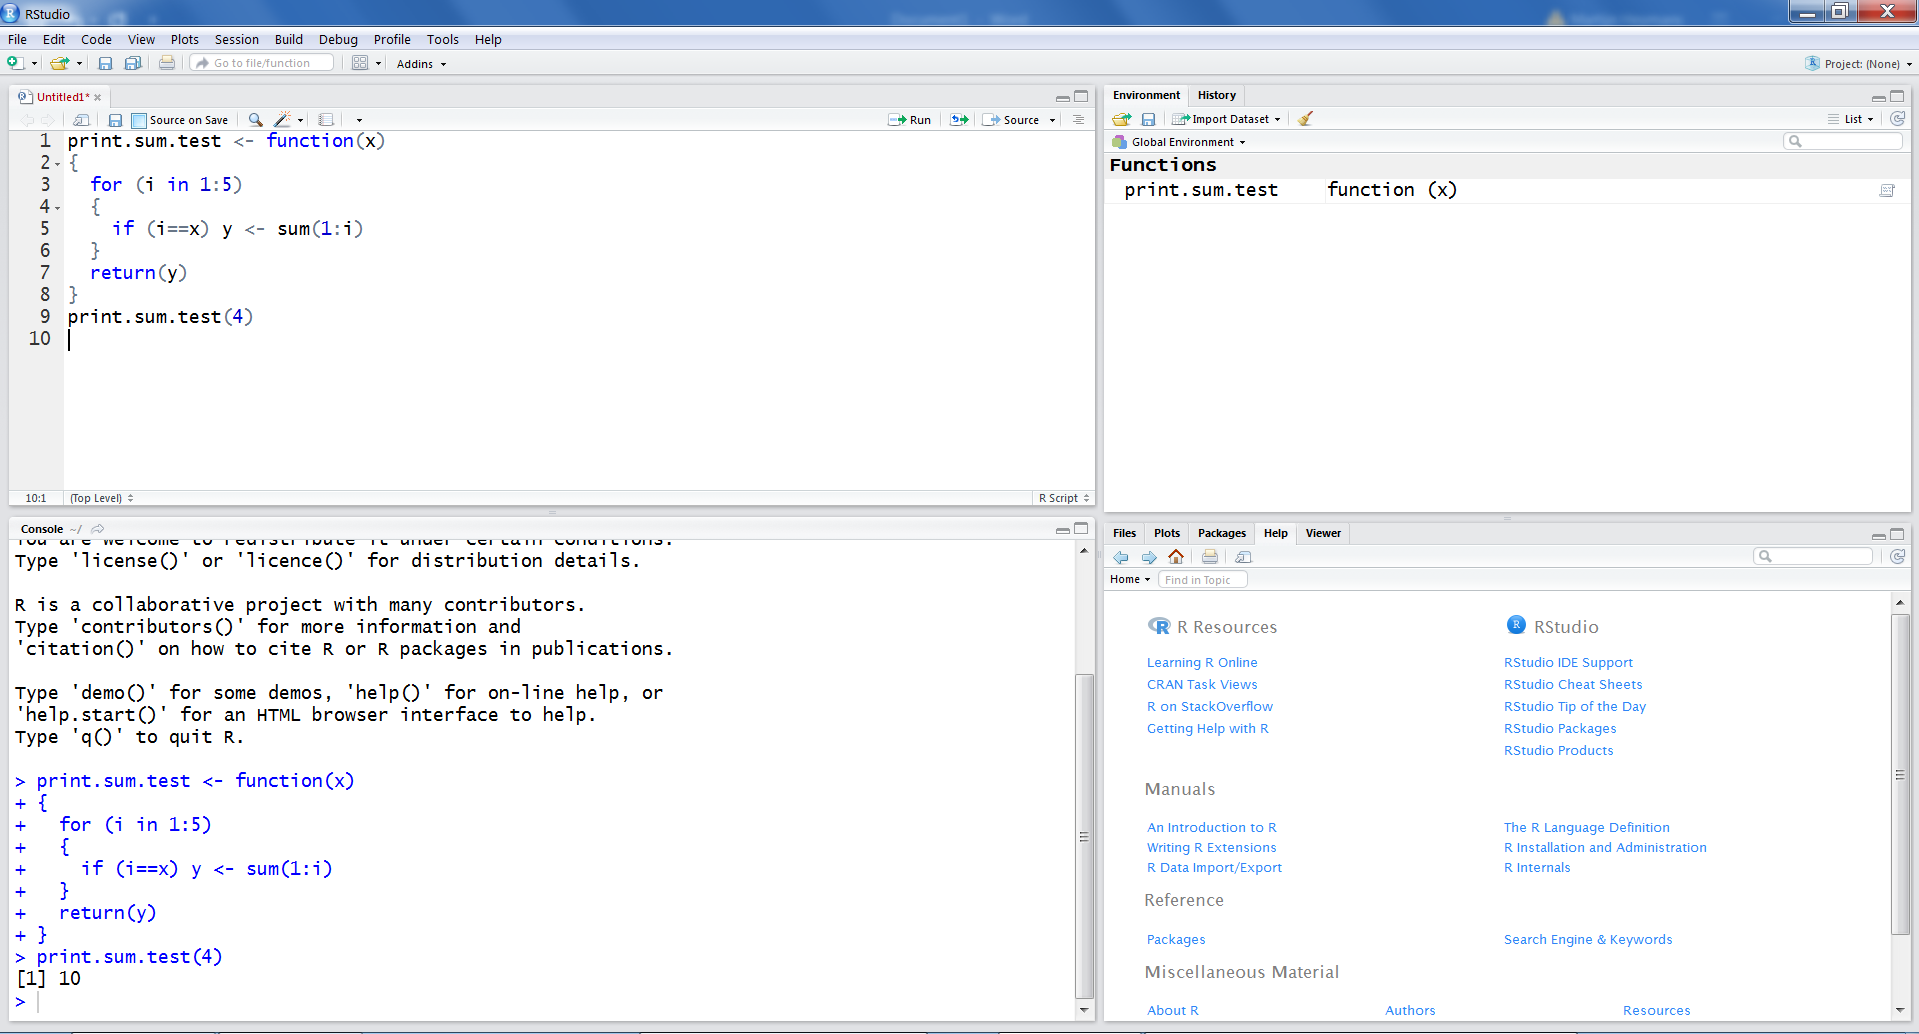
\includegraphics[width=0.9\linewidth]{images/fig1.11} 

}

\caption{Script file example in RStudio}\label{fig:fig11}
\end{figure}

\subsection{Creating a working
directory}\label{creating-a-working-directory}

It is a good idea to keep your R files at the same place when you are
doing data analysis for some kind of project. If you do not use a
separate directory, R will use a default directory, that will mostly be
in Windows in the documents folder. All files that you have to use
during your R session are assumed to be in that directory. Further, all
files that you save during your session will be in that directory. To
locate your working directory, you can type in the Console window:

\begin{Shaded}
\begin{Highlighting}[]
\KeywordTok{getwd}\NormalTok{()}
\end{Highlighting}
\end{Shaded}

In Rstudio there is another way to get information about the current
working directory and another way to change the working directory. Go in
RStudio to the window on the right site below and go to the Files tab
and click on the right site of the screen on the three dots. Than a
window will open and you can browse to your preferred folder. Then
choose for More in the Files tab and then select ``Set As Working
Directory'' (Figure \ref{fig:fig12}). Now you have set your preferred
working directory. You can check if your directory is set correctly by
choosing ``Go To Working Directory''.

\begin{figure}

{\centering 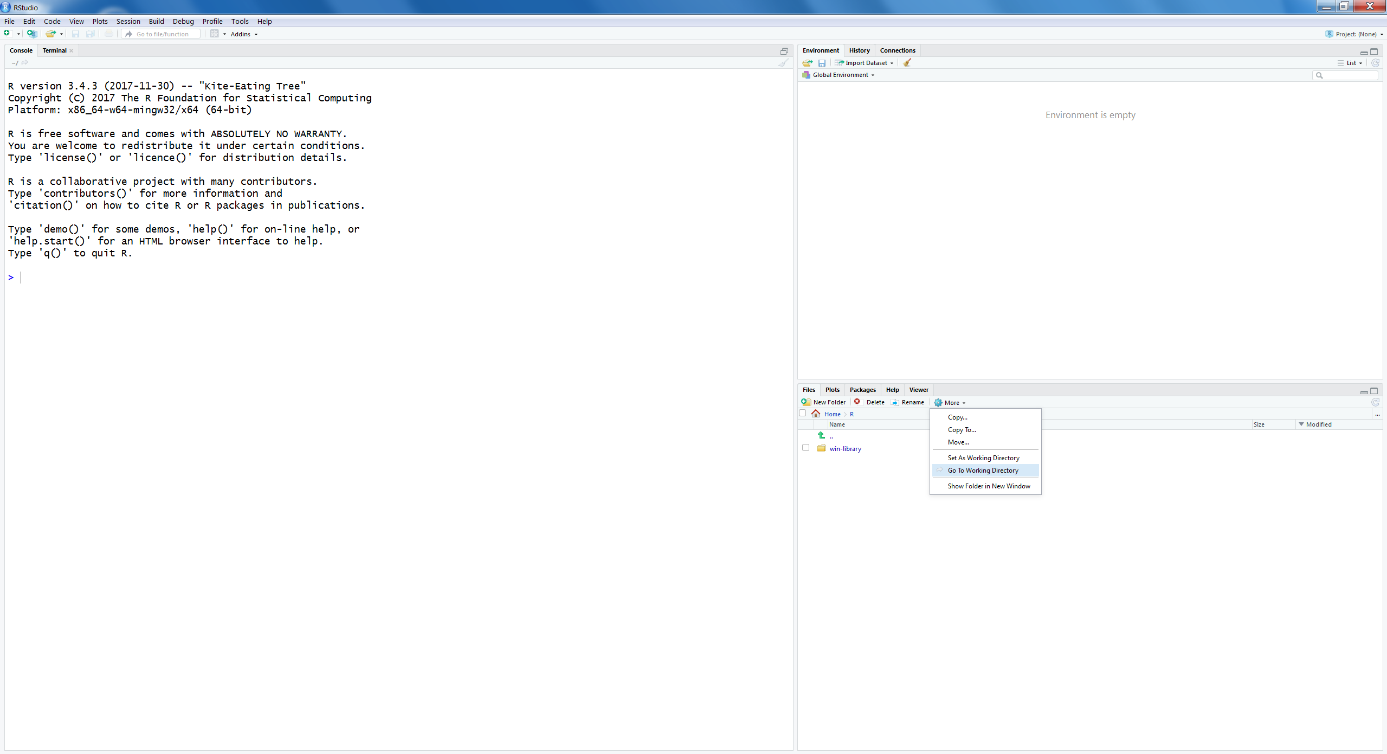
\includegraphics[width=0.9\linewidth]{images/fig1.12} 

}

\caption{Working directory selection in RStudio}\label{fig:fig12}
\end{figure}

\subsection{Reading in SPSS data in
RStudio}\label{reading-in-spss-data-in-rstudio}

There are several procedures in RStudio to read in datasets.

\begin{enumerate}
\def\labelenumi{\arabic{enumi}.}
\tightlist
\item
  Import datasets via ``Import Dataset'' An easy way to do that is via
  the window at the right site above. There you will find the button
  which is called ``Import Dataset''. When you click on it you can
  choose between different kind of file types, i.e.~CVS, Excel, SPSS,
  SAS and Stata files (Figure 1.13).
\end{enumerate}

\begin{figure}

{\centering 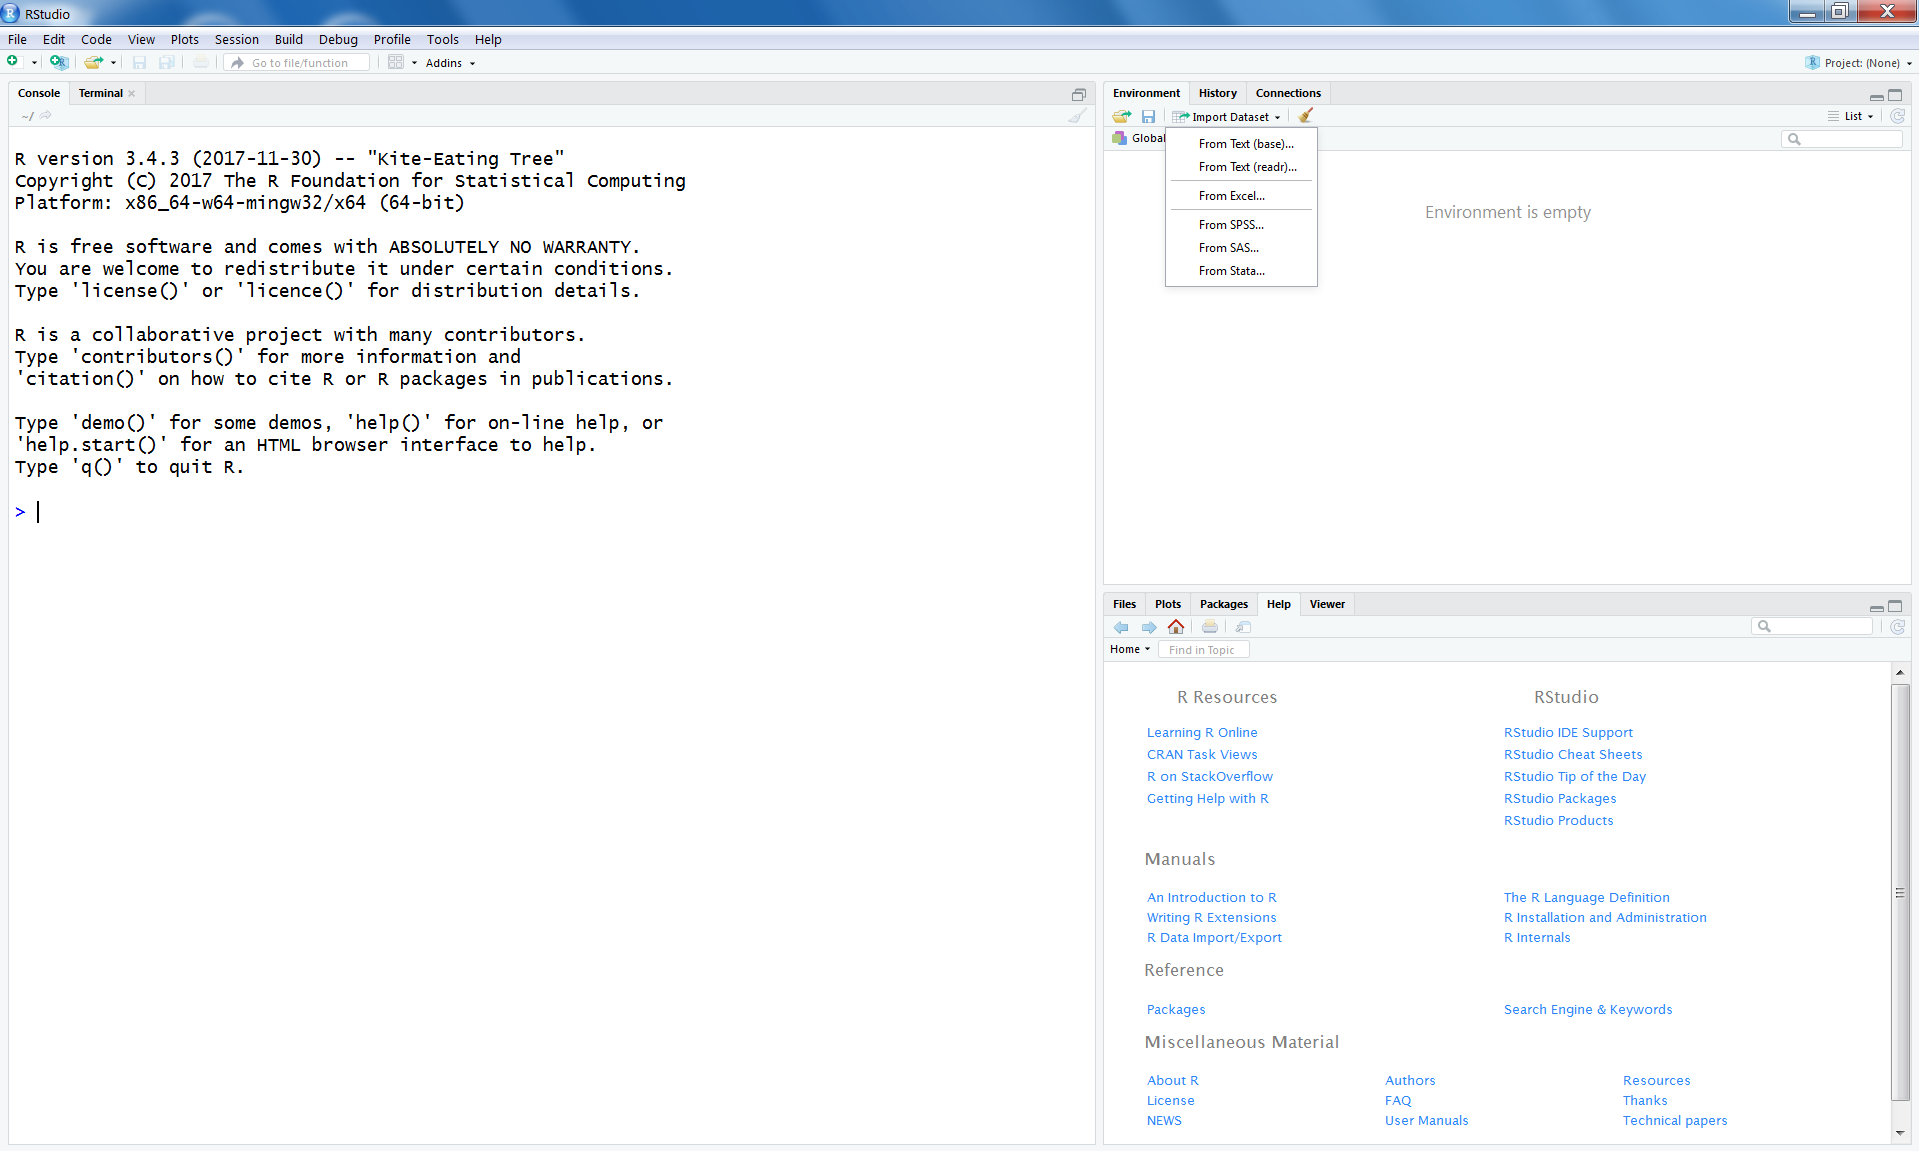
\includegraphics[width=0.9\linewidth]{images/fig1.13} 

}

\caption{Screen to import datasets in RStudio}\label{fig:fig13}
\end{figure}

In this example we choose for SPSS. When you approach this procedure for
the first time it could be that RStudio asks for your permission to
download a package called ``haven''. This package is built to import and
export data from several types. The following window will then appear
(Figure 1.14).

\begin{figure}

{\centering 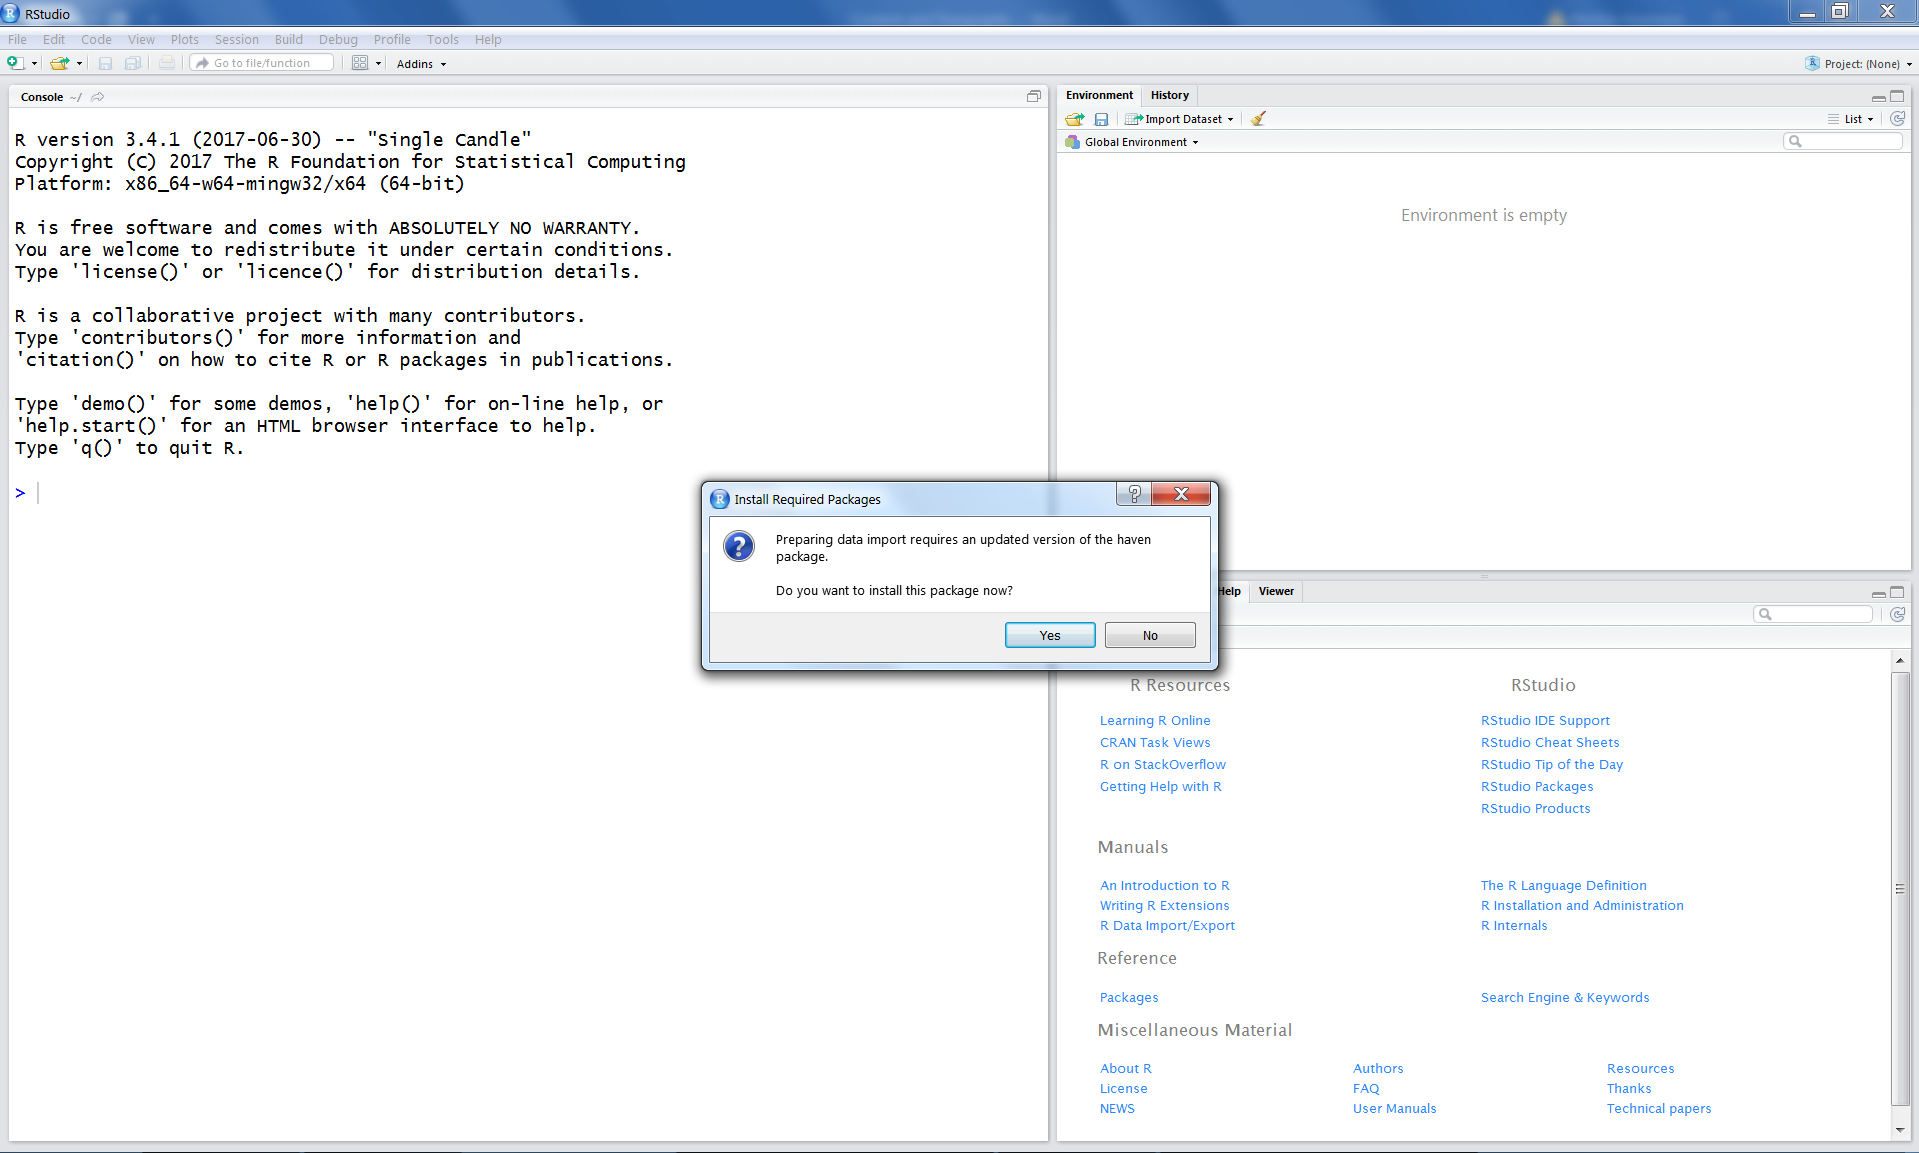
\includegraphics[width=0.9\linewidth]{images/fig1.14} 

}

\caption{Window to install the haven package}\label{fig:fig14}
\end{figure}

Click Yes and the download will start from the CRAN website. After the
package is installed a new window will open which is called ``Import
Statistical Data'' (Figure 1.15).

\begin{figure}

{\centering 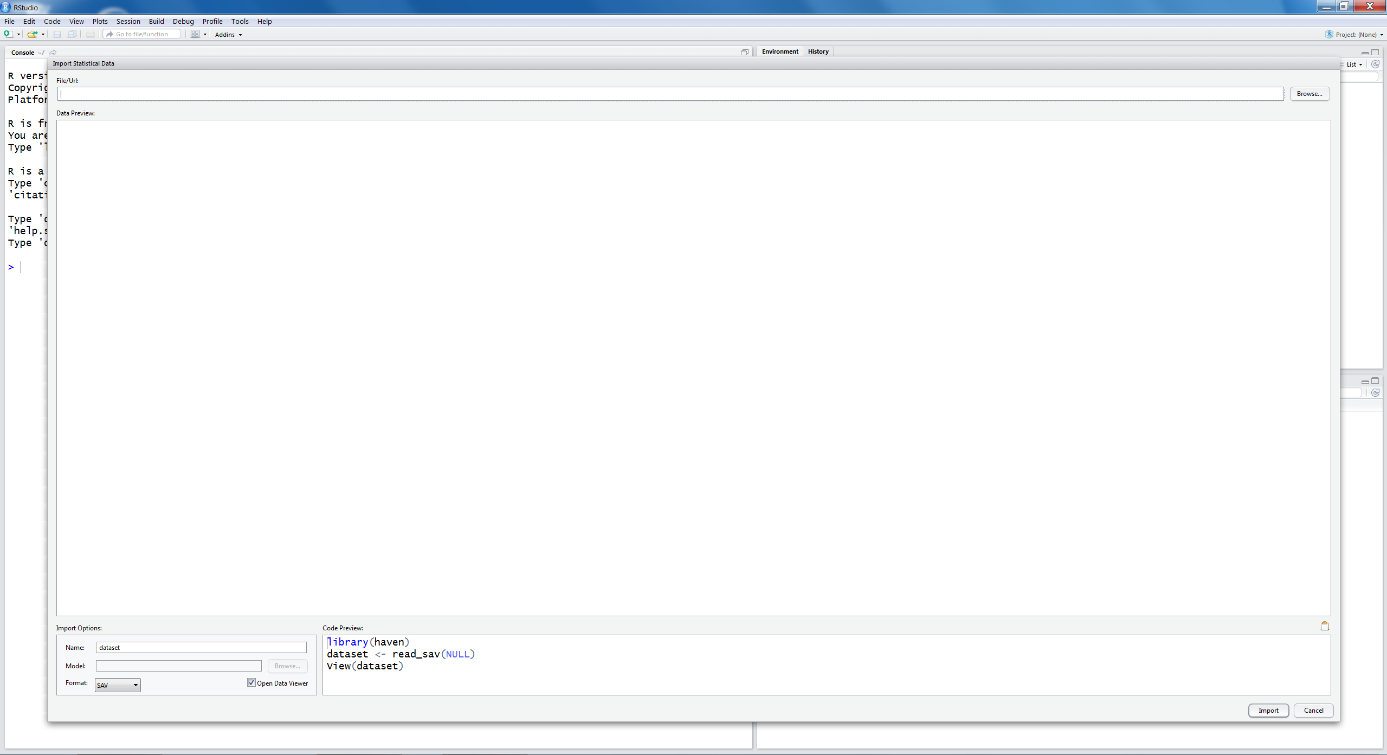
\includegraphics[width=0.9\linewidth]{images/fig1.15} 

}

\caption{The Import Statistical Data window in RStudio}\label{fig:fig15}
\end{figure}

At the top right site of the window you find the button which is called
``Browse''. That button allows you to browse to your dataset on your
computer. After you have opened your dataset you see a preview of your
dataset in RStudio (Figure 1.16).

\begin{figure}

{\centering 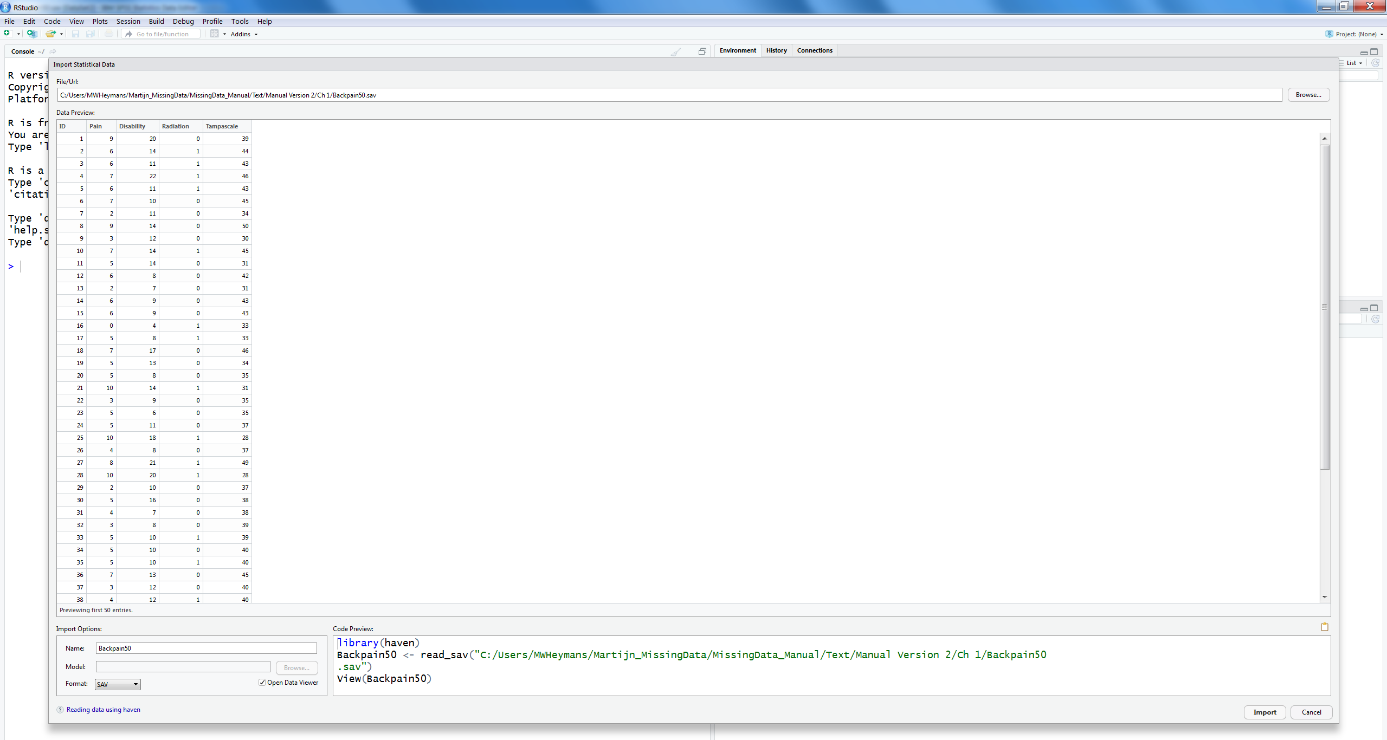
\includegraphics[width=0.9\linewidth]{images/fig1.16} 

}

\caption{A preview of the dataset in RStudio}\label{fig:fig16}
\end{figure}

Under Code Preview, under in the window, you see the code that was used
by RStudio to read in the dataset:

The dataset is automatically assigned to the object: Backpain50, which
is the original name of the dataset. When you click on Import, the
dataset is imported in the RStudio environment (Figure 1.17).

\begin{figure}

{\centering 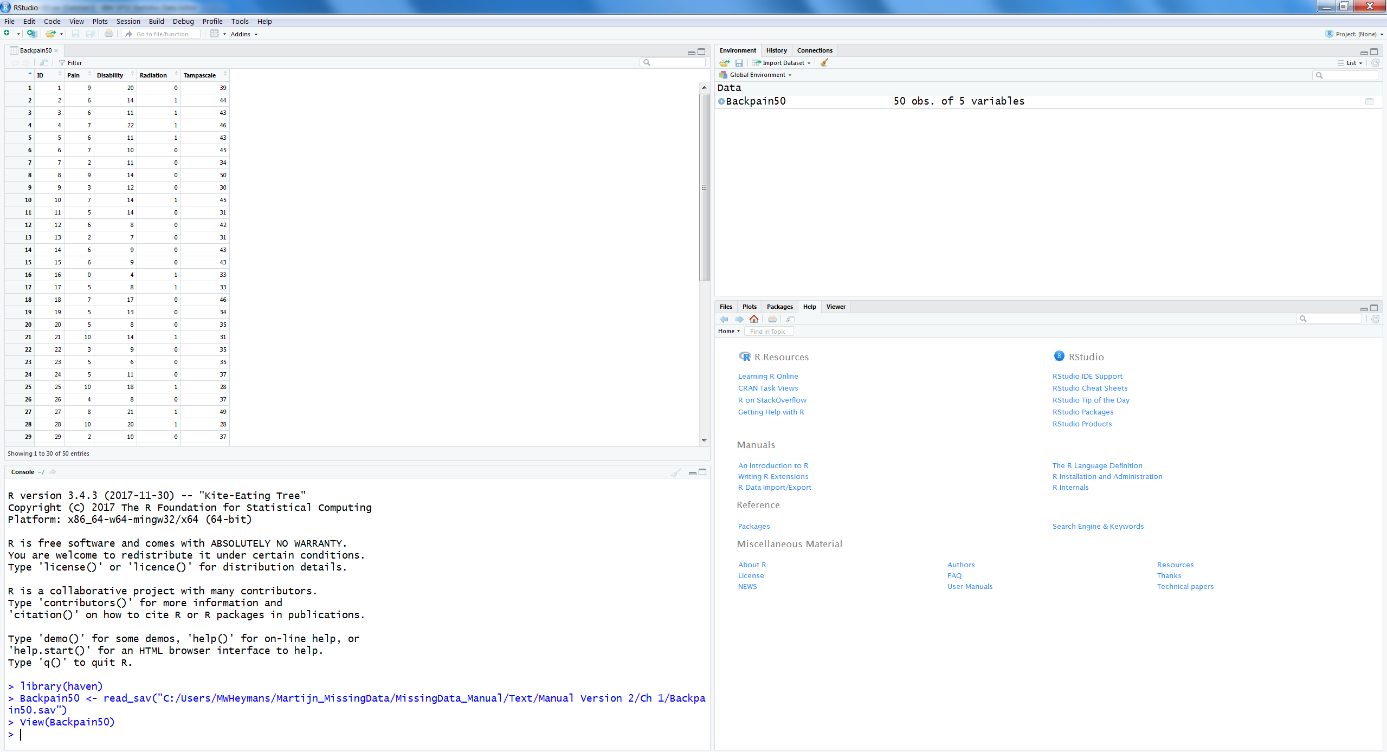
\includegraphics[width=0.9\linewidth]{images/fig1.17} 

}

\caption{Imported dataset in RStudio}\label{fig:fig17}
\end{figure}

Another way to import an SPSS dataset is by making use of the foreign
package. You can find this package under the Packages Tab in the window
at the right site below under the heading ``System Library''. Install
that package first. The foreign package includes the function
``read.spss''. Let's first explore the function arguments of this
function by using:

Now the following information can be found in the right window below,
under the Help tab:

read.spss(file, use.value.labels = TRUE, to.data.frame = FALSE,
max.value.labels = Inf, trim.factor.names = FALSE, trim\_values = TRUE,
reencode = NA, use.missings = to.data.frame)

The most important arguments to change for us are the file and
to.data.frame arguments. When you are in the correct working directory,
i.e.~the working directory where the file that you want to import is
stored, you use the following code to import the dataset:

\subsection{Saving and Reading R data in
RStudio}\label{saving-and-reading-r-data-in-rstudio}

Datasets can be saved and read in R using different commands.

\emph{Write.table} and \emph{Read.table}

\emph{Write.table} The write.table function can be used to write
matrices and data frames (datasets) to the working directory. The R code
is:

Files that have been written with write.table can be easily read in, in
SPSS by using the steps that will be discussed in the next paragraph.

\emph{Read.table} The read.table function can be used to read in
matrices and data frames by using:

\emph{Save and Load}

\emph{Save} You can also use the command save to save datasets,
according to (notice the .RData extension):

\emph{Load} Loading the dataset again in the workspace can be done by
using:

You can also use save by using the default options in the following way
to save your datasets:

To get direct access to the data that you have saved, you can use the
get function in combination with the load function like this:

With save, you can save any R object, also lists such as:

Subsequently, after you have removed object x from the workspace, you
can load it again by using:

\subsection{Reading in (R)Studio data into
SPSS}\label{reading-in-rstudio-data-into-spss}

When you have used the write.table function to save data in R you can
easily read them in into SPSS. First you have to use write.table in the
following way:

The extra parameter settings, mean: sep=``;'', separate each variable by
an ``;'' indicator. dec=``,'', use for decimals a ``,'' instead of an
``.''. row.names=F , Do not add an extra column with row.names.

Follow the next steps to read in the data into SPSS: choose File
-\textgreater{} Open data -\textgreater{} ``All files (\emph{.})'', than
you will see the file you want to read in into SPSS. In this example we
will use the file ``Backpain50 R file'' from R code 1.41 (Figure 1.18).

\begin{figure}

{\centering 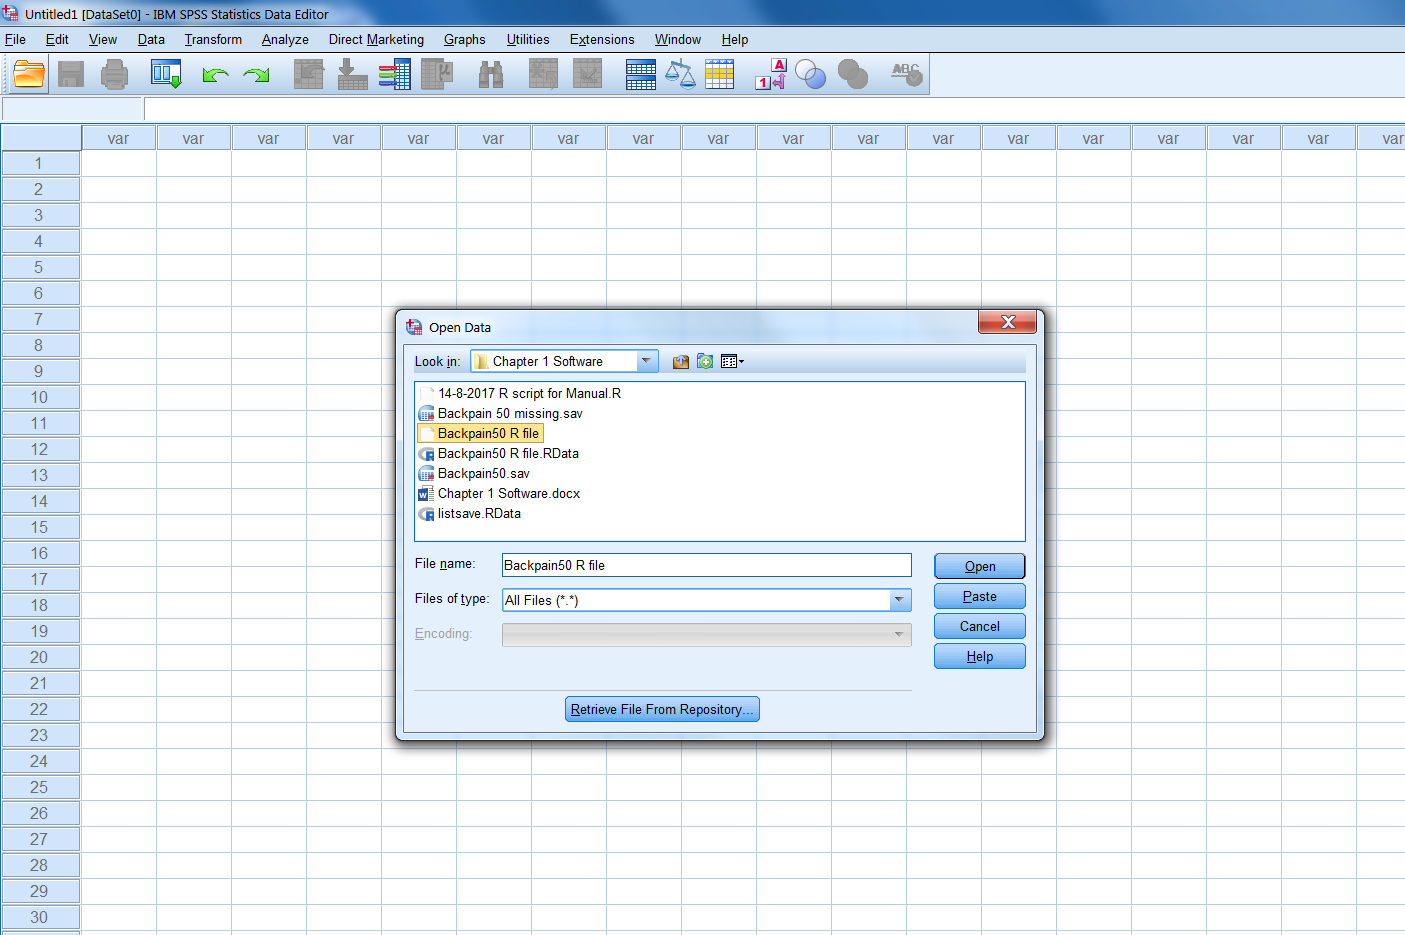
\includegraphics[width=0.9\linewidth]{images/fig1.18} 

}

\caption{Choosing the dataset to import in SPSS}\label{fig:fig18}
\end{figure}

Then click Open (wait a couple of seconds) and click on next. You will
see the following window that is part of the Text Import Wizard
procedure in SPSS (Figure 1.19):

\begin{figure}

{\centering 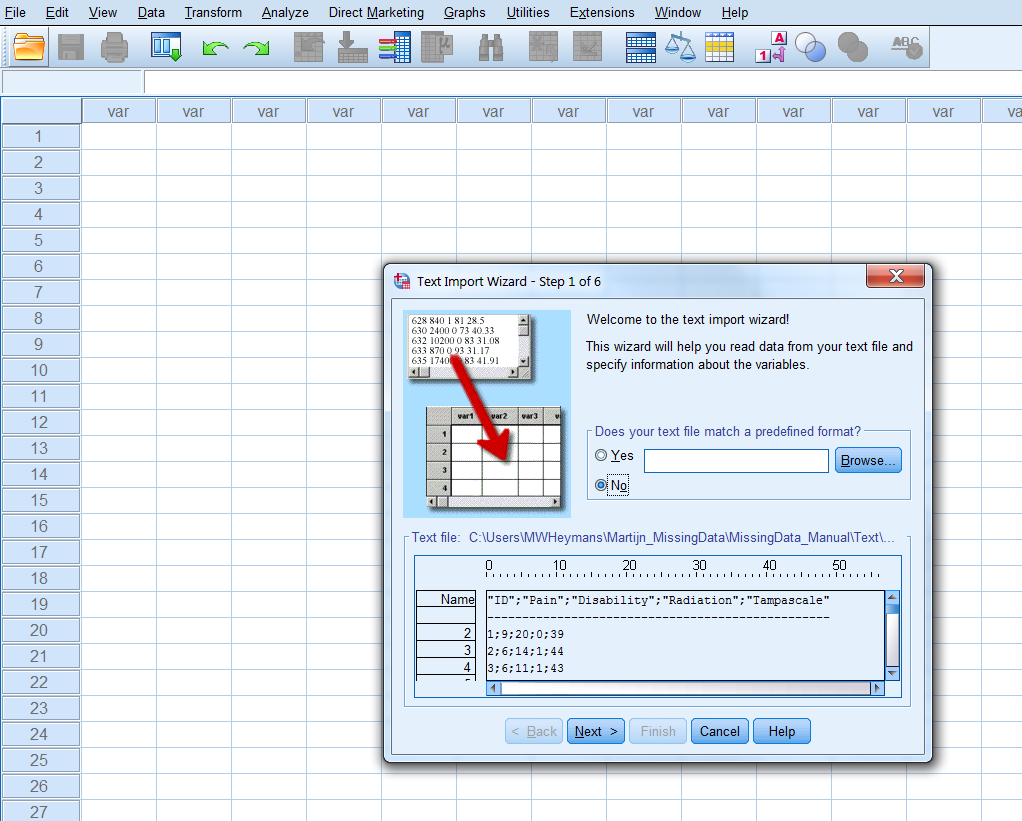
\includegraphics[width=0.9\linewidth]{images/fig1.19} 

}

\caption{Step 1 of the Text Import Wizard}\label{fig:fig19}
\end{figure}

Then click the ``Next \textgreater{}'' button 5 times, passing by the
following windows:

Step 2 of 6 (Figure 1.20): To change how variables are arranged: here
delimited To include variable names included at the top of the file:
here Yes. To set the decimal symbol: here a comma.

\begin{figure}

{\centering 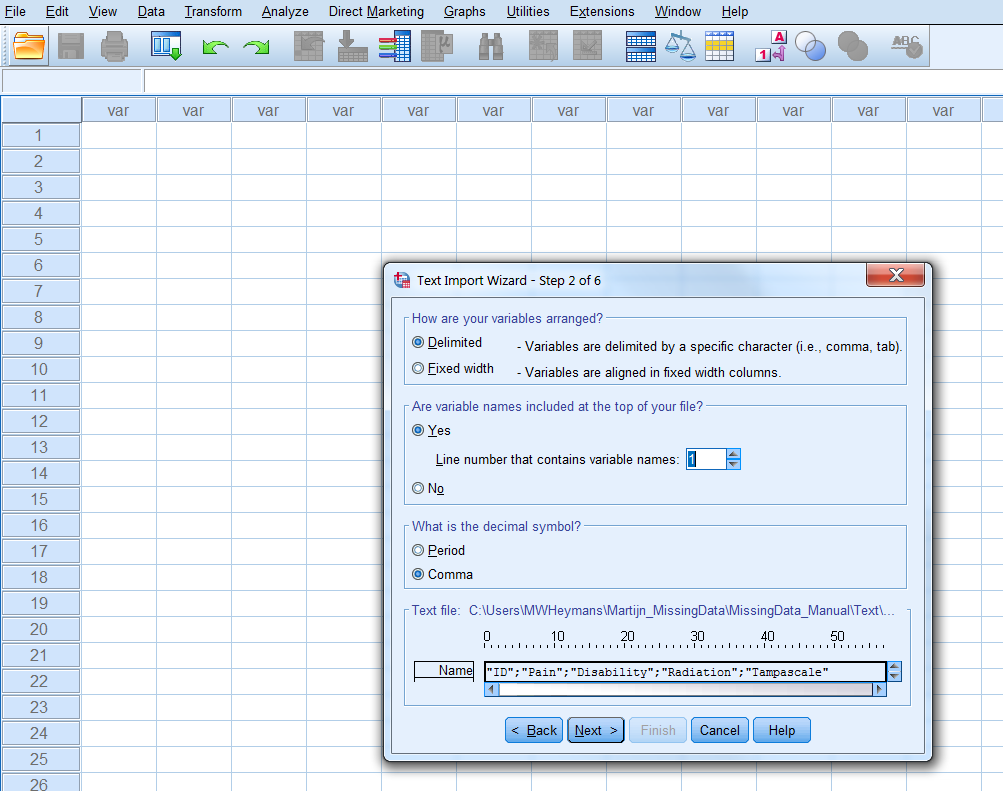
\includegraphics[width=0.9\linewidth]{images/fig1.20} 

}

\caption{Step 2 of the Text Import Wizard}\label{fig:fig20}
\end{figure}

Step 3 of 6 (Figure 1.21):

On which line number begins the first case: here 2 How cases are
represented: Each line is a case. How many cases you want to import:
here all cases.

\begin{figure}

{\centering 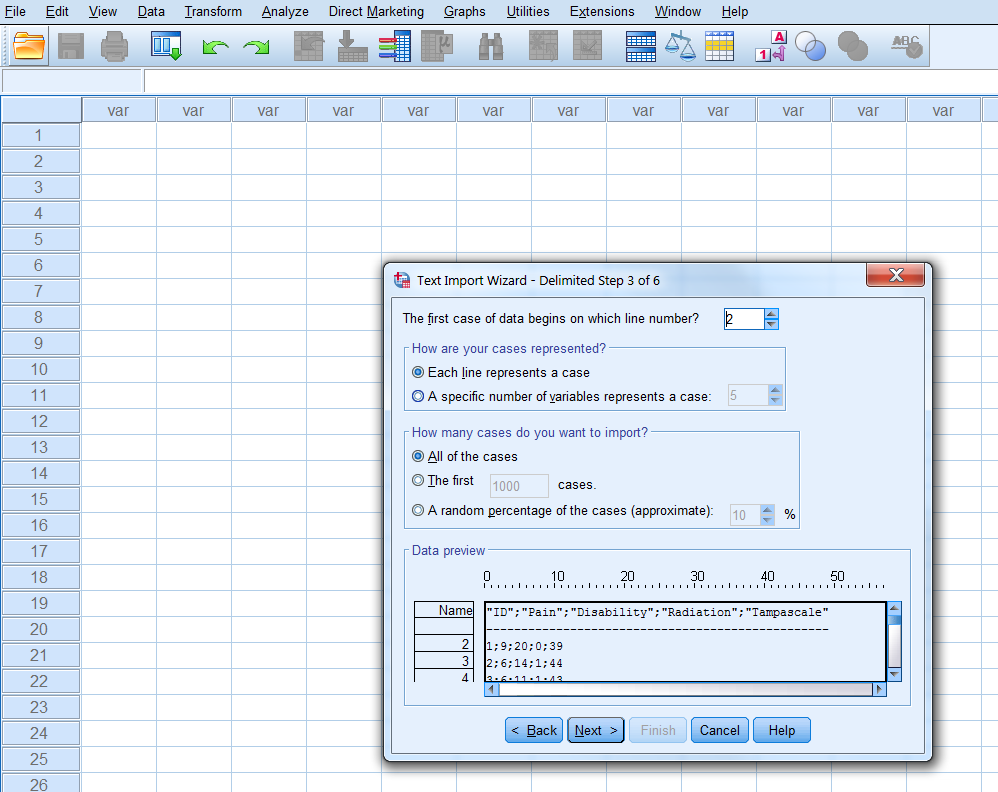
\includegraphics[width=0.9\linewidth]{images/fig1.21} 

}

\caption{Step 3 of the Text Import Wizard}\label{fig:fig21}
\end{figure}

Step 4 of 6 (Figure 1.22): The delimiters that appear between variables;
here the Semicolon. The text qualifier: here Double quote. Remove
trailing spaces from string values: skip.

\begin{figure}

{\centering 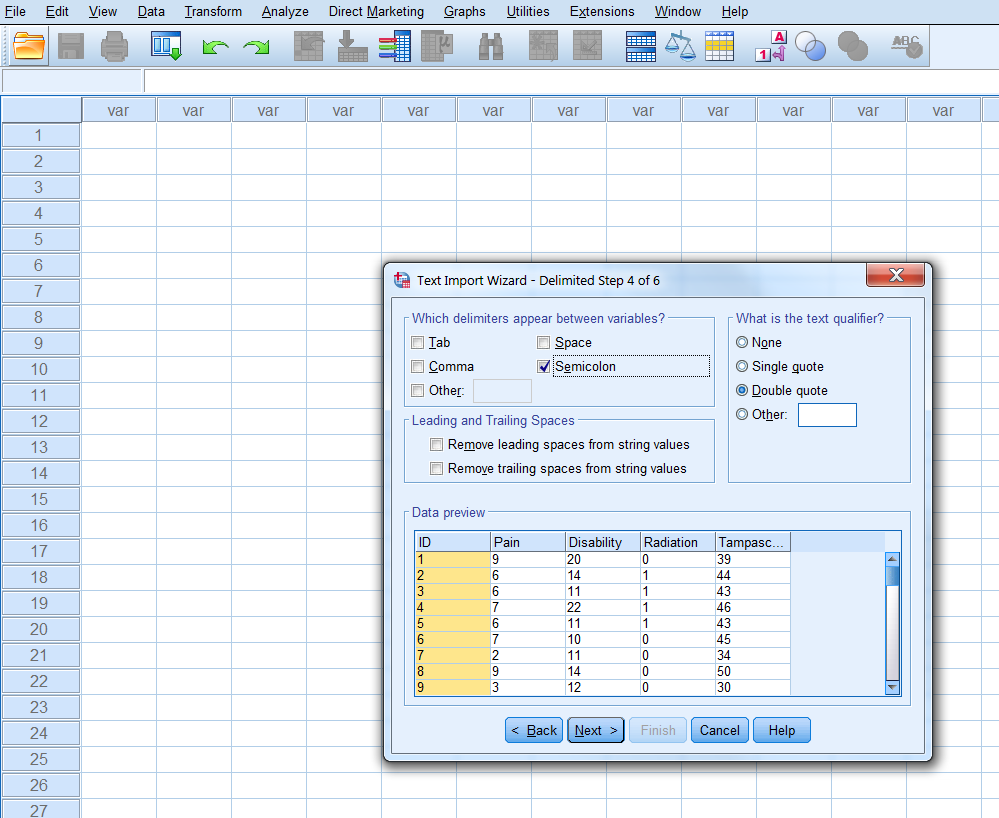
\includegraphics[width=0.9\linewidth]{images/fig1.22} 

}

\caption{Step 4 of the Text Import Wizard}\label{fig:fig22}
\end{figure}

Step 5 of 6 (Figure 1.23): Here you can overwrite the Data format of the
variable (you can also change that in the Variable View window, when the
data has been read in).

\begin{figure}

{\centering 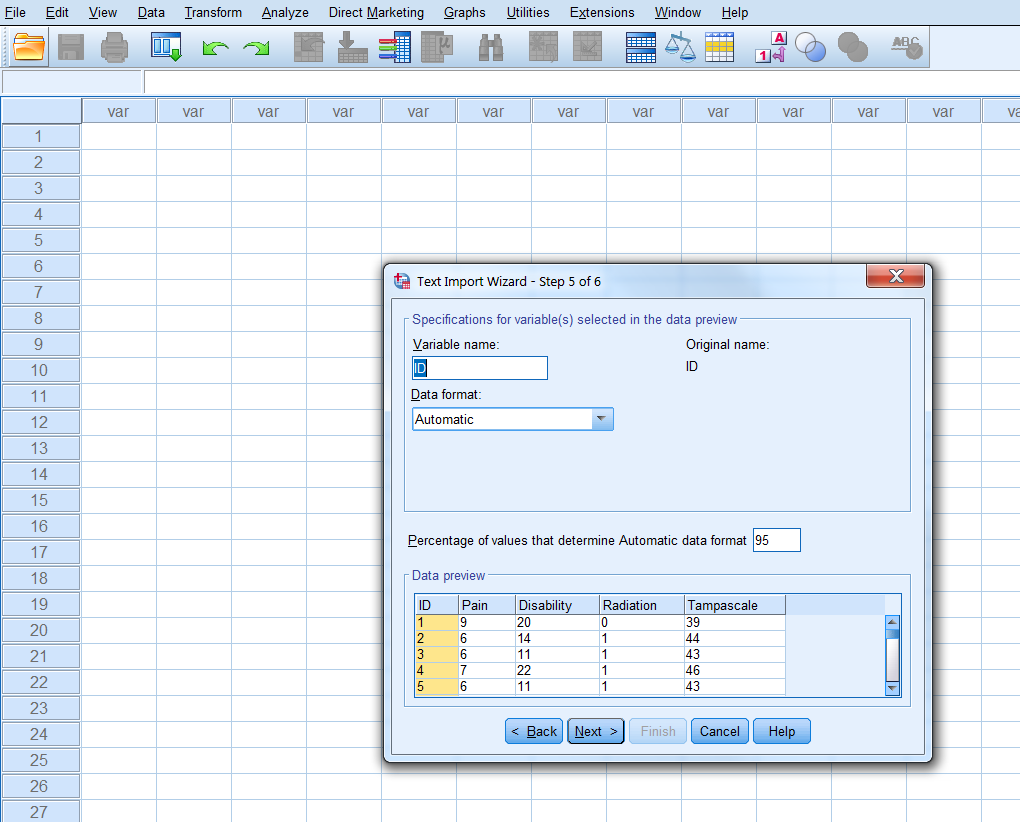
\includegraphics[width=0.9\linewidth]{images/fig1.23} 

}

\caption{Step 5 of the Text Import Wizard}\label{fig:fig23}
\end{figure}

Step 6 of 6: This step allows you to save your specifications of the
previous steps into a separate file (Figure 1.24).

\begin{figure}

{\centering 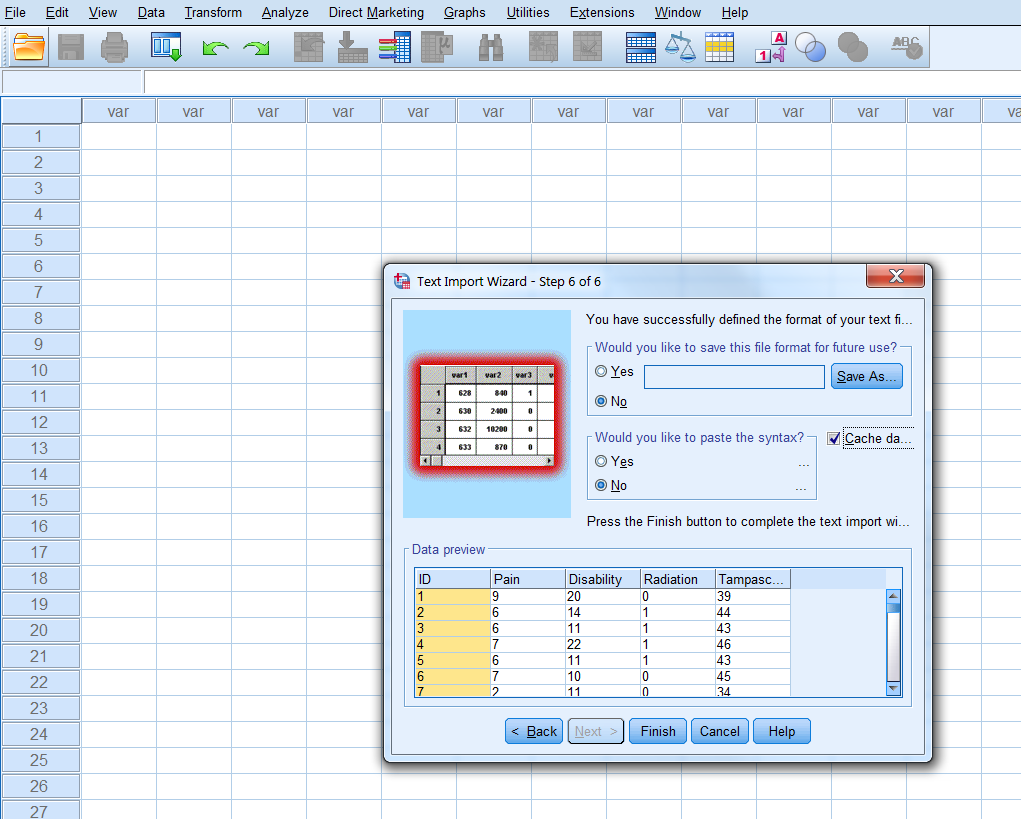
\includegraphics[width=0.9\linewidth]{images/fig1.24} 

}

\caption{Step 6 of the Text Import Wizard}\label{fig:fig24}
\end{figure}

Then click finish and the data will be read in, into a new SPSS file. In
that file you can of course change all kind of variable and data
settings in the Variable View Window.

You can also skip step 2 to 5 by clicking the Finish button twice when
you are at step 1. Than you use all default settings, which is most of
the times a good option.

\subsection{Installing R Packages}\label{installing-r-packages}

When R is installed on your computer also a folder called library is
created. This folder contains packages that are part of the basic
installation. A package is a collection of different functions written
in the R language. Besides packages that are part of the basic
installation of R there are also packages that are not part of the basic
installation but are written by others, i.e.~the add-on packages.
Packages can be downloaded from the CRAN website
(\url{https://cran.r-project.org/}). Currently, there are thousands of
user-written packages available on the CRAN website.

Before you can use a specific package that is not part of the basic
installation, you have to install it in your R library. In this manual
we will use the mice package to do all kind of imputation procedures,
such as multiple imputation. mice is not part of the basic installation
so we have to install it first. There are several procedures in RStudio
to install a package. One way is to use the install.packages function in
the Console window as follows:

The mice package will be automatically downloaded from the CRAN website.

Another way is to use the window on the right site below and go to the
Packages tab. When you click ``Install'' a new window is opened. Than
you can type ``mice'' on the blank line under ``Packages (separate
multiple with space or comma):'' (Figure 1.25a and b).

\begin{figure}

{\centering 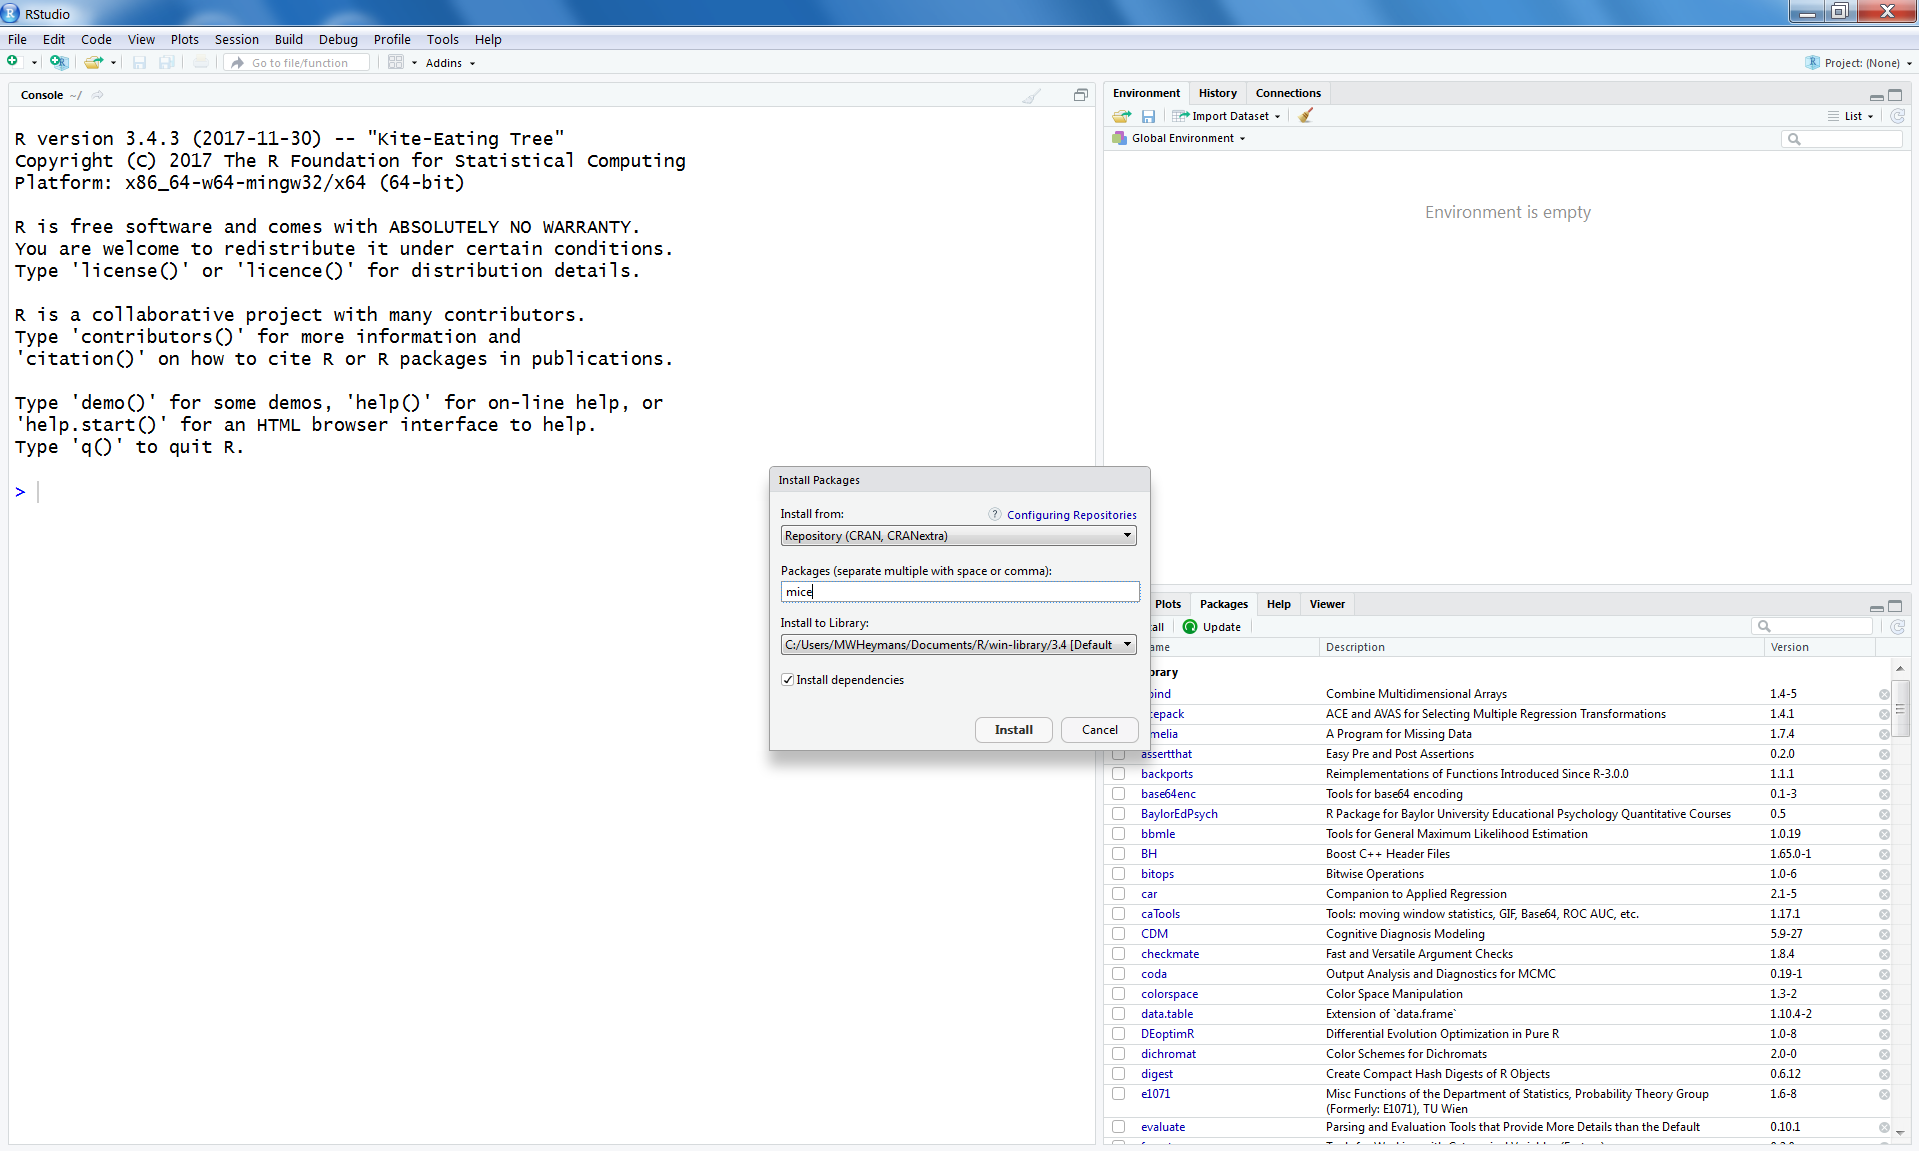
\includegraphics[width=0.9\linewidth]{images/fig1.25a} 

}

\caption{Install packages Window in RStudio to install packages from the CRAN website}\label{fig:fig25}
\end{figure}

\begin{figure}

{\centering 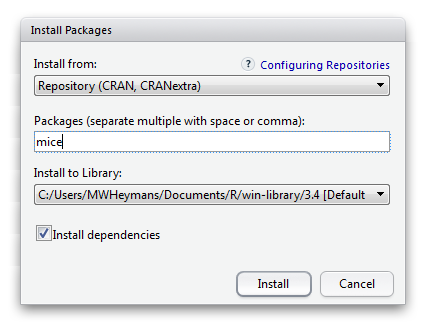
\includegraphics[width=0.9\linewidth]{images/fig1.25b} 

}

\caption{Enlarged Install packages Window in RStudio to install packages from the CRAN website}\label{fig:fig26}
\end{figure}

After you have clicked on ``Install'' the package will be downloaded
from the CRAN website automatically and will be listed in the Package
list named ``User Library''.

Another way is to go to the CRAN website and download the package as a
zip file in a directory on your computer, for example your working
directory or in your library. Again use the window on the right site
below and go to the Packages tab. When you choose Install a new window
is opened. Now under ``Install from:'' choose for ``Package Archive File
(.zip; .tar.gz)'' (Figure 1.26a and 1.26b). Than you can browse to the
zip file and install the package.

\begin{figure}

{\centering 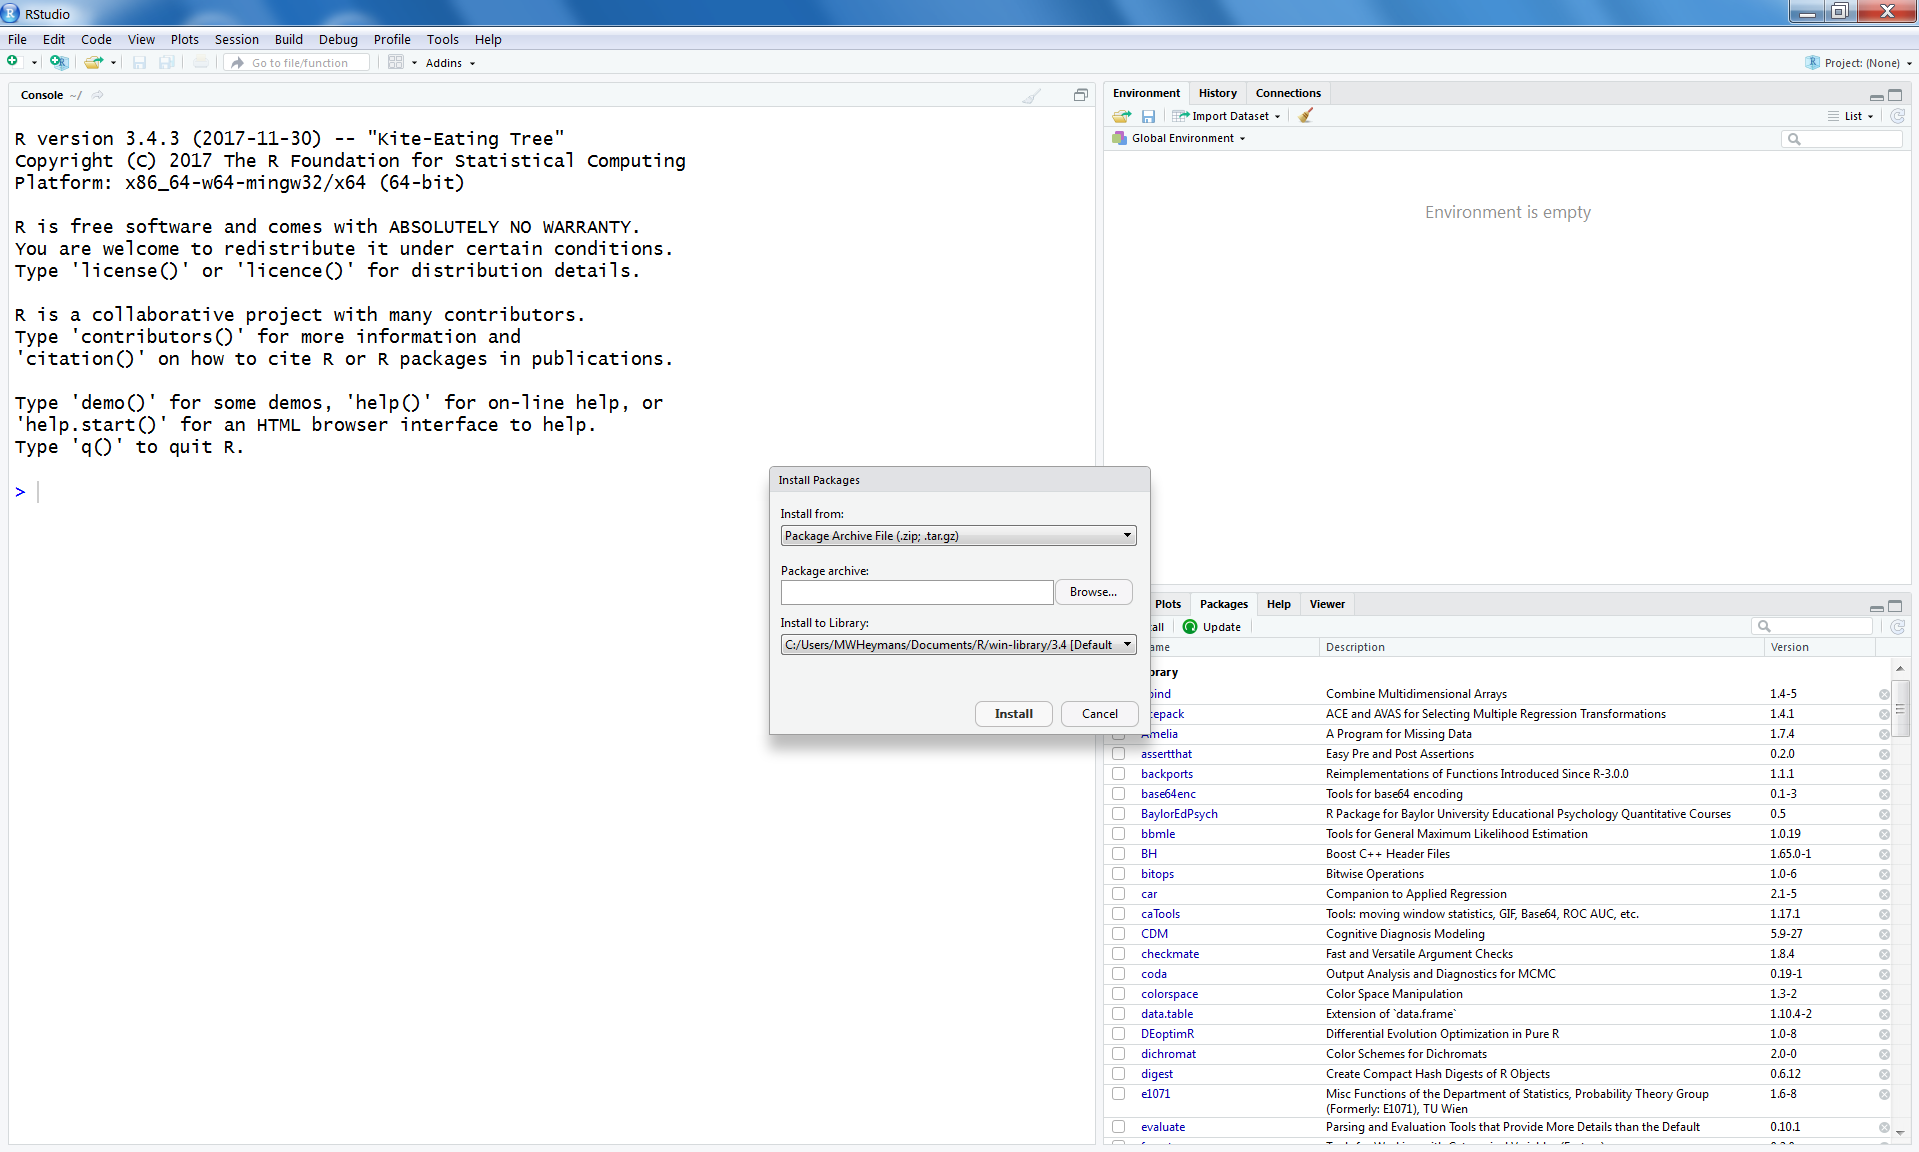
\includegraphics[width=0.9\linewidth]{images/fig1.26a} 

}

\caption{Install packages Window in RStudio to install packages from zip files}\label{fig:fig27}
\end{figure}

\begin{figure}

{\centering 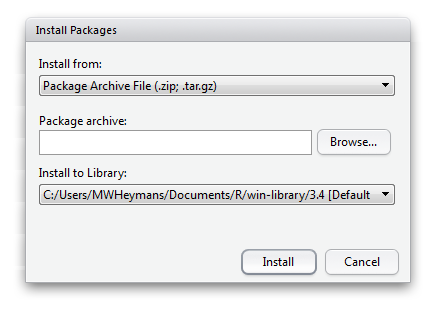
\includegraphics[width=0.9\linewidth]{images/fig1.26b} 

}

\caption{Enlarged Install packages Window in RStudio to install packages from zip files}\label{fig:fig28}
\end{figure}

\subsection{Loading R Packages}\label{loading-r-packages}

Once an add-on (user written) R package has been installed it has to be
loaded to get access to all functions that are part of that package. To
load a library, you can use the function library() or require(). R code
1.43 shows an example of loading the mice package.

The require() function is used in the same way. You have to load add-on
packages each time you start a new R session.

\subsection{Updating R Packages}\label{updating-r-packages}

To keep the add-on packages up to date you can use the update.packages()
function in R. R code 1.44 presents an example.

R will ask you if you want to update each package. If you type ``y'' in
the Console window, R will update the package.

In RStudio updating packages can be done in the Package tab as well. You
can click on the Update button. A new window will open that contains a
list of all packages that need to be updated. Subsequently you can
select the packages you want to update.

\subsection{Useful Missing data Packages and
links}\label{useful-missing-data-packages-and-links}

The main package that we will use in this manual is mice which stand for
Multivariate Imputation by Chained Equations (MICE) (Van Buuren, 2009).

Other packages that are related to MICE are miceadds and micemd:
miceadds: this package contains some additional multiple imputation
functions (Robitzsch et al., 2017). See for more information:
\href{https://cran.r-project.org/web/packages/miceadds/index.html}{linked
phrase}

micemd: this package contains additional functions for the mice package
to perform multiple imputation in two-level (Multilevel) data (Audigier
\& Resche-Rigon, 2017). See for more information:
\href{https://cran.r-project.org/web/packages/micemd/index.html}{linked
phrase}

mi: provides functions for data manipulation, imputing missing values in
an approximate Bayesian framework, diagnostics of the models used to
generate the imputations, confidence-building mechanisms to validate
some of the assumptions of the imputation algorithm, and functions to
analyze multiply imputed data sets (Gelman et al., 2015). See for more
information:
\href{https://cran.r-project.org/web/packages/mi/index.html}{linked
phrase}

MItools: small package to perform analyses and combine results from
multiple-imputation datasets (Lumley, 2015). See for more information:
\href{https://cran.r-project.org/web/packages/mitools/index.html}{linked
phrase}

norm: this package is for the Analysis of multivariate normal datasets
with missing values. It contains the mi.inference function. This
function combines estimates and standard errors to produce a single
inference. Uses the technique described by Rubin (1987), which are
called the Rubin's Rules (RR) (Novo, 2015). See for more information:
\href{https://cran.r-project.org/web/packages/norm/index.html}{linked
phrase}

vim (visualization and imputation of missing values): This package
includes tools for the visualization of missing and/or imputed values.
In addition, the quality of imputation can be visually explored using
various univariate, bivariate, multiple and multivariate plot methods
(Templ et al., 2017). See for more information:
\href{https://cran.r-project.org/web/packages/mi/index.html}{linked
phrase}

BaylorEdPsych: R Package for Baylor University Educational Psychology
Quantitative Courses. This package included Little's MCAR test
(Beaujean, 2015). See for more information:
\href{https://cran.r-project.org/web/packages/BaylorEdPsych/index.html}{linked
phrase}

MKmisc: Contains several functions for statistical data analysis;
e.g.~for sample size and power calculations, computation of confidence
intervals, and generation of similarity matrices. This package contains
the mi.t.test function for pooling t-tests after multiple imputation
(Kohl, 2016). See for more information:
\href{https://cran.r-project.org/web/packages/MKmisc/index.html}{linked
phrase}

mvnmle: This package estimates the maximum likelihood estimate of the
mean vector and variance-covariance matrix for multivariate normal data
with missing values. This package is needed for the mlest function this
is used for Little's MCAR test in Cahpter 2. See for more information:
\href{https://cran.r-project.org/web/packages/mvnmle/index.html}{linked
phrase}

\chapter{Missing Data Evaluation}\label{missing-data-evaluation}

Before you decide what to do with your missing data it is important to
consider the reasons and probable causes of your missing data problem.
With that information you can compose an analysis plan to deal with the
missing data in your dataset. In this Chapter, you will learn how to
explore and evaluate your missing data in SPSS and R and why it is
important to think about the missing data mechanism. This knowledge is
important for the method you choose to handle the missing data problem.

\section{Definition of Missing Data}\label{definition-of-missing-data}

\subsection{Defining Missing Data in
SPSS}\label{defining-missing-data-in-spss}

Missing data in SPSS can be defined in two ways, as a system missing or
user missing value. System missing data is missing data that is not
present in the dataset and can be recognized by an empty cell (or dot).
User missing data is data that is coded as missing value in the dataset
by the user for some specific kind of reason. As an example we use a
small dataset with 50 Backpain patients consisting of males (coded as 1)
and females (coded as 0) patients (Figure \ref{fig:fig2-1}). The female
patients in this dataset have been pregnant and the Gestational Age (GA)
variable, contains the duration of their pregnancy in weeks.

\begin{figure}

{\centering 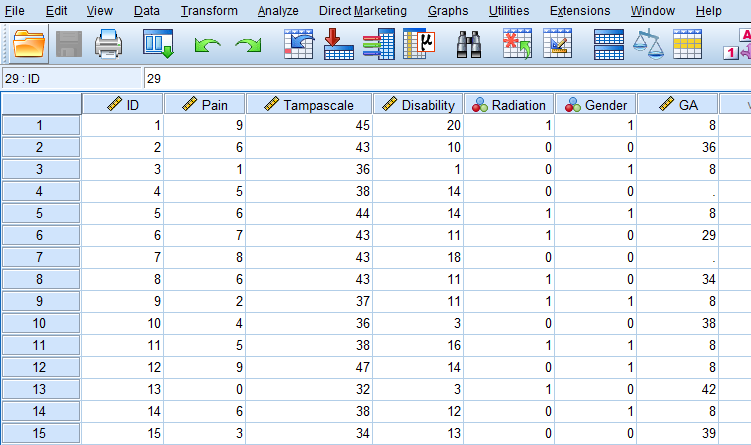
\includegraphics[width=0.9\linewidth]{images/fig2.1} 

}

\caption{SPSS dataset containing variables with system and user missing data}\label{fig:fig2-1}
\end{figure}

The Variable GA in the dataset consists of different values, like real
values for GA as 36 and 29, the value 8 and empty cells. The value 8 is
specified by us to exclude males from further analysis that include the
GA variable. This is a user missing value, that was indicated because
males cannot be pregnant. The system missing values are recognizable by
the empty cells (or dots) in the dataset, and these indicate the missing
GA values for women who did not report their GA. It makes no difference
if we code the missing values as a system or user missing value in SPSS,
because both kinds of missing values are recognized as missing values by
SPSS and will be excluded from further analyses.

\subsection{Missing data in R}\label{missing-data-in-r}

In R the missing values are denoted by NA which means ``Not Available''.
If we open the same dataset as above in R we get the following result.

\begin{Shaded}
\begin{Highlighting}[]
\KeywordTok{library}\NormalTok{(haven)}
\NormalTok{dataset <-}\StringTok{ }\KeywordTok{read_sav}\NormalTok{(}\StringTok{"data/CH2 example.sav"}\NormalTok{)}
\KeywordTok{head}\NormalTok{(dataset,}\DecValTok{10}\NormalTok{)}
\end{Highlighting}
\end{Shaded}

\begin{verbatim}
## # A tibble: 10 x 7
##       ID  Pain Tampascale Disability Radiation Gender    GA
##    <dbl> <dbl>      <dbl>      <dbl>     <dbl>  <dbl> <dbl>
##  1     1     9         45         20         1      1     8
##  2     2     6         43         10         0      1    36
##  3     3     1         36          1         0      1     8
##  4     4     5         38         14         0      0    NA
##  5     5     6         44         14         1      1     8
##  6     6     7         43         11         1      0    29
##  7     7     8         43         18         0      0    NA
##  8     8     6         43         11         1      0    34
##  9     9     2         37         11         1      1     8
## 10    10     4         36          3         0      0    38
\end{verbatim}

The Variable Gestational Age (GA) contains the values for GA (e.g.~36,
29, etc.), the value 8 for males and the NA's. In R the value 8 will be
treated as a real value, so we have to recode that value to NA by using
the following code.

\begin{Shaded}
\begin{Highlighting}[]
\NormalTok{dataset}\OperatorTok{$}\NormalTok{GA[dataset}\OperatorTok{$}\NormalTok{GA}\OperatorTok{==}\DecValTok{8}\NormalTok{] <-}\StringTok{ }\OtherTok{NA}
\KeywordTok{head}\NormalTok{(dataset,}\DecValTok{10}\NormalTok{)}
\end{Highlighting}
\end{Shaded}

\begin{verbatim}
## # A tibble: 10 x 7
##       ID  Pain Tampascale Disability Radiation Gender    GA
##    <dbl> <dbl>      <dbl>      <dbl>     <dbl>  <dbl> <dbl>
##  1     1     9         45         20         1      1    NA
##  2     2     6         43         10         0      1    36
##  3     3     1         36          1         0      1    NA
##  4     4     5         38         14         0      0    NA
##  5     5     6         44         14         1      1    NA
##  6     6     7         43         11         1      0    29
##  7     7     8         43         18         0      0    NA
##  8     8     6         43         11         1      0    34
##  9     9     2         37         11         1      1    NA
## 10    10     4         36          3         0      0    38
\end{verbatim}

The \texttt{NA} values will be recognized as missing values. For most
functions in R the handling of \texttt{NA} values has to be defined. For
example, the following code to obtain the mean of Gestational Age
results in an \texttt{NA} because the handling of missing data is not
defined.

\begin{Shaded}
\begin{Highlighting}[]
\KeywordTok{mean}\NormalTok{(dataset}\OperatorTok{$}\NormalTok{GA)}
\end{Highlighting}
\end{Shaded}

\begin{verbatim}
## [1] NA
\end{verbatim}

To obtain the mean of the observed data the following code has to be
used:

\begin{Shaded}
\begin{Highlighting}[]
\KeywordTok{mean}\NormalTok{(dataset}\OperatorTok{$}\NormalTok{GA, }\DataTypeTok{na.rm=}\OtherTok{TRUE}\NormalTok{)}
\end{Highlighting}
\end{Shaded}

\begin{verbatim}
## [1] 35.09524
\end{verbatim}

The \texttt{na.rm=TRUE} statement in the mean-function, indicates that
values that are NA need to be removed before the analysis can be
executed. Another NA handling procedure that is used in functions is
called na.action with as options \texttt{na.fail}, \texttt{na.omit},
\texttt{NULL} (no action) and \texttt{na.exclude}. For more information
about na.action options you can type the following code in the R console
\texttt{?na.action}.

\section{Missing data Patterns}\label{missing-data-patterns}

To get an idea about the complexity of the missing data problem in your
dataset and information about the location of the missing values, the
missing data pattern can be evaluated. Historically, the missing data
pattern was important as a starting point to choose the missing data
handling method (Little and Rubin, 2002). Currently, the missing data
pattern is less important because the most advanced (missing) data
analysis methods as multiple imputation can handle almost any missing
data pattern. We will discuss some frequently seen missing data
patterns, which are graphically displayed in Figure \ref{fig:fig2-2}.

\begin{figure}

{\centering 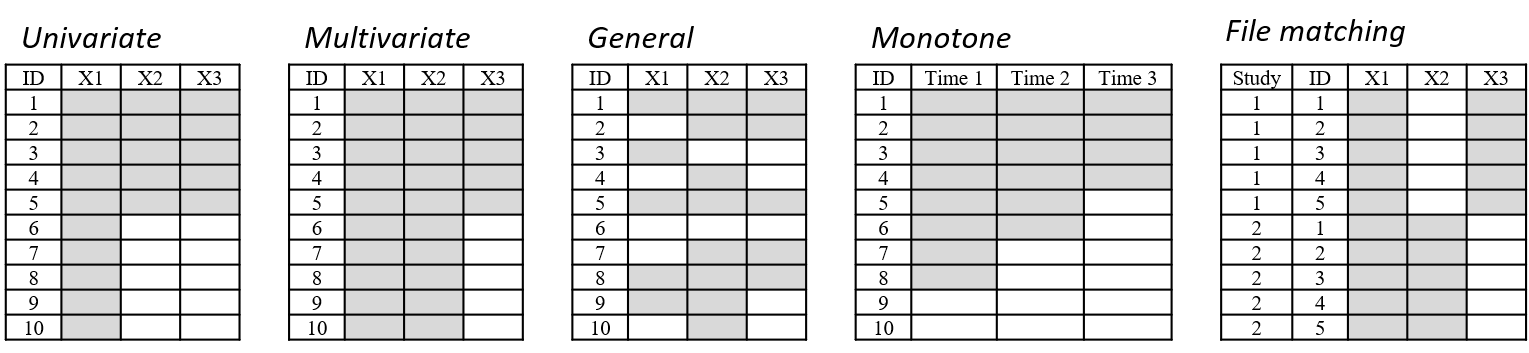
\includegraphics[width=0.9\linewidth]{images/fig2.2} 

}

\caption{Missing data patterns (ID means person identification number, X1 to X3 represent variables, Time 1 to 3 means that data is measured at 3 time points over time, Study means study number). The white cells represent the missing data}\label{fig:fig2-2}
\end{figure}

A univariate missing data pattern is a pattern with missing values in
only one variable. An example of such a pattern is when the independent
variables are completely observed, but the outcome variable is not, or
when a selection of subjects refuse to fill in a specific question such
as their income level. The second and third pattern are examples of
multivariate missing data patterns, where multiple variables contain
missing values. The second pattern is an example where subjects miss
values of the same two variables and the third pattern a more general
pattern where different subject miss different variable scores. A
monotone pattern of missing data may occur in a longitudinal study with
data repeatedly assessed over time, and subjects ``drop-out'' of the
study (fourth pattern). An example could be an elderly study where
persons become too frail to participate or just because persons do not
want to attend the study anymore because they are not interested to fill
in several questionnaires. A pattern called File Matching can be
observed when data from several studies is merged for an individual
participant data analysis and variables are not assessed in all studies.
In our example, one variable is observed in both studies (X1), but X2
and is only observed in study 1 and X3 in study 2.

\subsection{Missing data patterns in
SPSS}\label{missing-data-patterns-in-spss}

To evaluate the missing data pattern, we can make use of the options
under the Missing Value Analysis (MVA) procedure in SPSS (IBM, 2016). We
use as an example a dataset that contains information of 150 Back pain
patients and 9 study variables. The variables are Pain (continuous),
Tampa scale (continuous), Radiation in the leg (dichotomous), Disability
(continuous), Body Weight (continuous), Body Length (continuous), Age
(continuous), Smoking (dichotomous), Gender (dichotomous). Only the
variables Gender and Age are completely observed.

To access the MVA function in the SPSS menu choose:
\textgreater{}Analyze -\textgreater{} Missing Value Analysis\ldots{}

A new window will open that is called ``Missing Value Analysis'' (Figure
\ref{fig:fig2-3})

\begin{figure}

{\centering 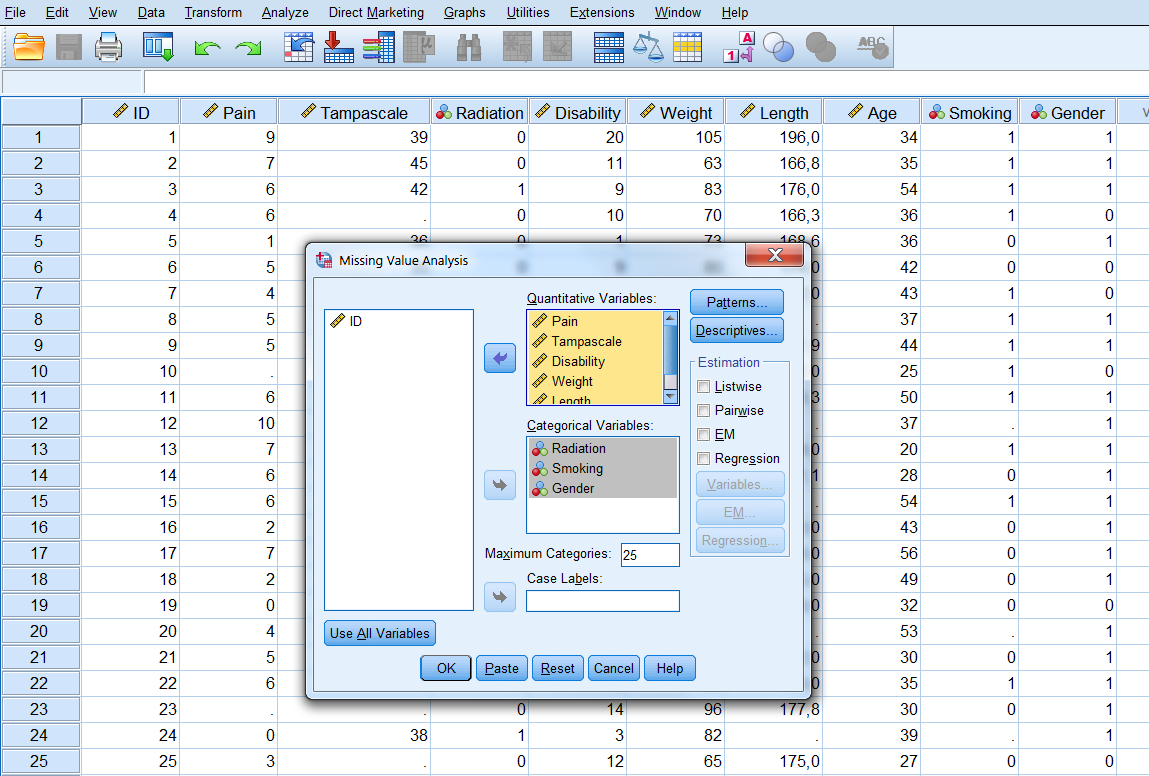
\includegraphics[width=0.9\linewidth]{images/fig2.3} 

}

\caption{The Missing Value Analysis menu}\label{fig:fig2-3}
\end{figure}

From this menu we first transfer all variables of interest in the
correct Quantitative and Categorical variables window and then choose
for the Patterns option. From the Patterns menu choose for the options
\texttt{Tabulated\ cases,\ grouped\ by\ missing\ value\ patterns} and
\texttt{sort\ variables\ by\ missing\ value\ pattern}. To obtain the
full list of all patterns that occur in the data, set the ``Omit
patterns with less than 1\% of cases at 0\%, then click on continue and
OK. This will produce the output table that is displayed in Figure
\ref{fig:tab2-1}.

\begin{figure}

{\centering 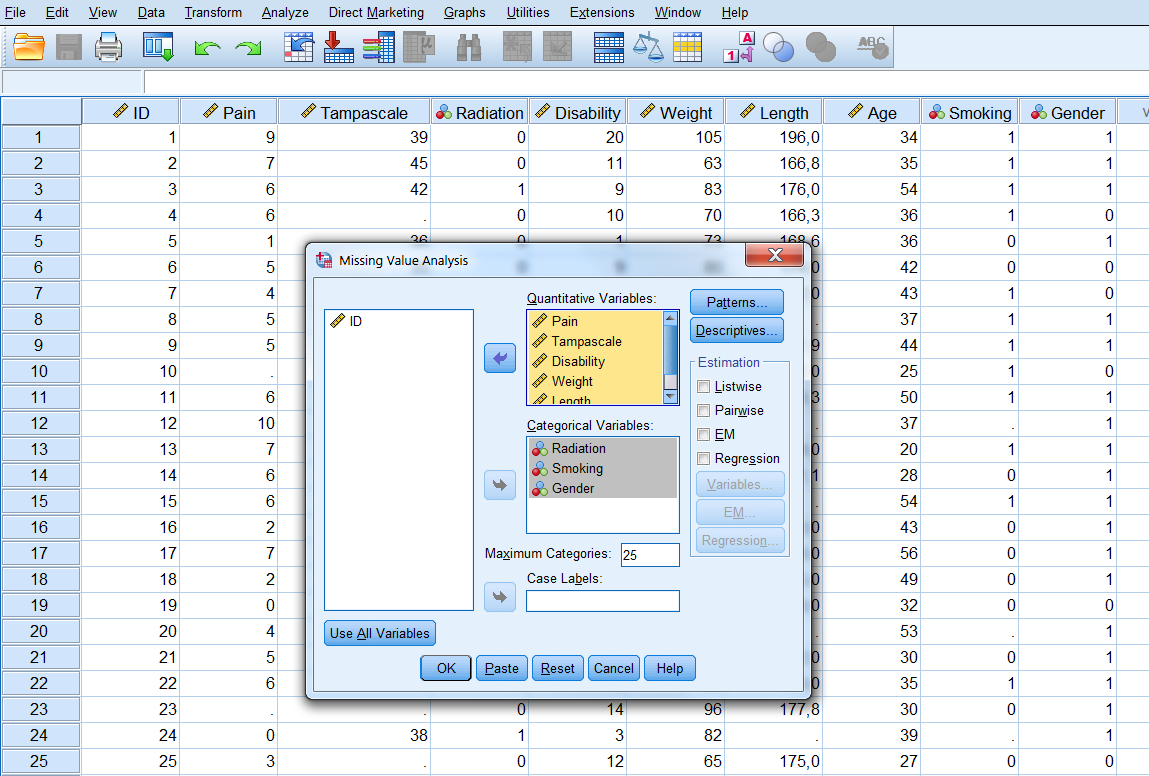
\includegraphics[width=0.9\linewidth]{images/fig2.3} 

}

\caption{The Patterns menu}\label{fig:fig2-4}
\end{figure}

From this menu we first transfer all variables of interest in the
correct Quantitative and Categorical variables window and then choose
for the Patterns option. From the Patterns menu choose for the options
``Tabulated cases, grouped by missing value patterns'' and ``sort
variables by missing value pattern''. To obtain the full list of all
patterns that occur in the data, set the ``Omit patterns with less than
1\% of cases at 0\%, then click on continue and OK. This will produce
the output table that is displayed in Tables 2.1a and 2.1b.

\begin{figure}

{\centering 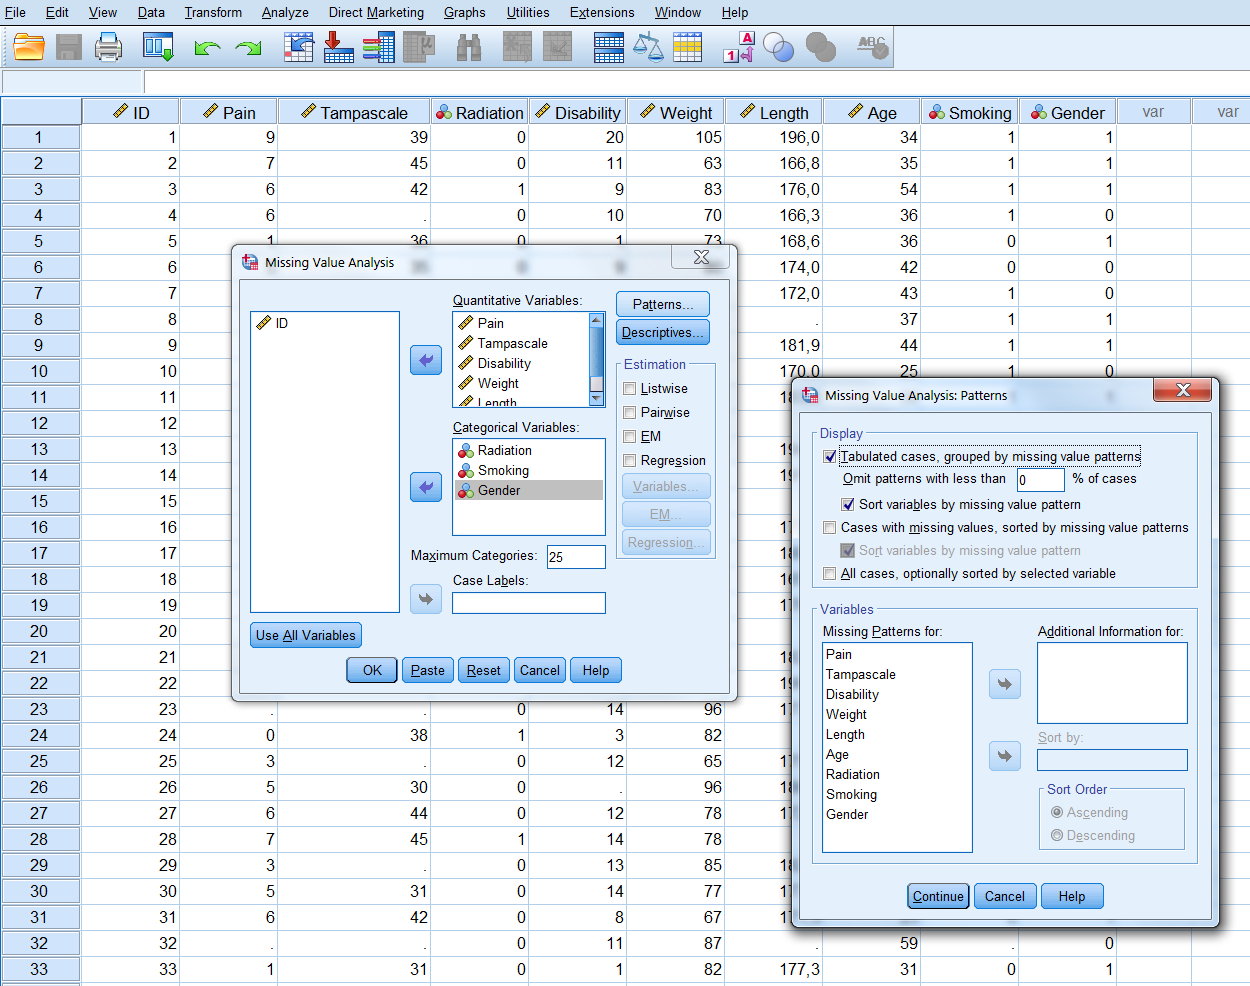
\includegraphics[width=0.9\linewidth]{images/fig2.4} 

}

\caption{The Patterns menu}\label{fig:fig30}
\end{figure}

As default procedure univariate statistics are presented including
output information about the number and percentages of missing data and
other descriptive statistics for each variable. Information about the
missing data patterns is provided in the Tabulated patterns table. On
the left column of that table, named ``Number of Cases'', the number of
cases are presented with that specific missing data pattern. In our
example, there are 75 cases in total without any missing values and 13
cases with a missing value in only the Tampa scale variable (see row 1
and 2 of Table 2.1). In the right column of that table named ``Complete
if\ldots{}'', the total number of subjects is presented if the variables
that contain missing data in that pattern are not used in the analysis.
Those variables are marked with the ``X'' symbol. For example, 88
subjects will be included in the analysis when the variable Tampa scale
is not used in the analysis, those are the 75 subjects that have
completely observed data on top of the 13 subjects with missing data in
the Tampa scale variable only.

\begin{figure}

{\centering 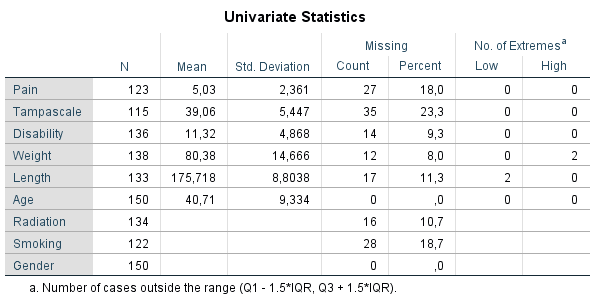
\includegraphics[width=0.9\linewidth]{images/tab2.1a} 

}

\caption{Descriptive missing data statistics and the missing data patterns.}\label{fig:tab2-1}
\end{figure}\begin{figure}

{\centering 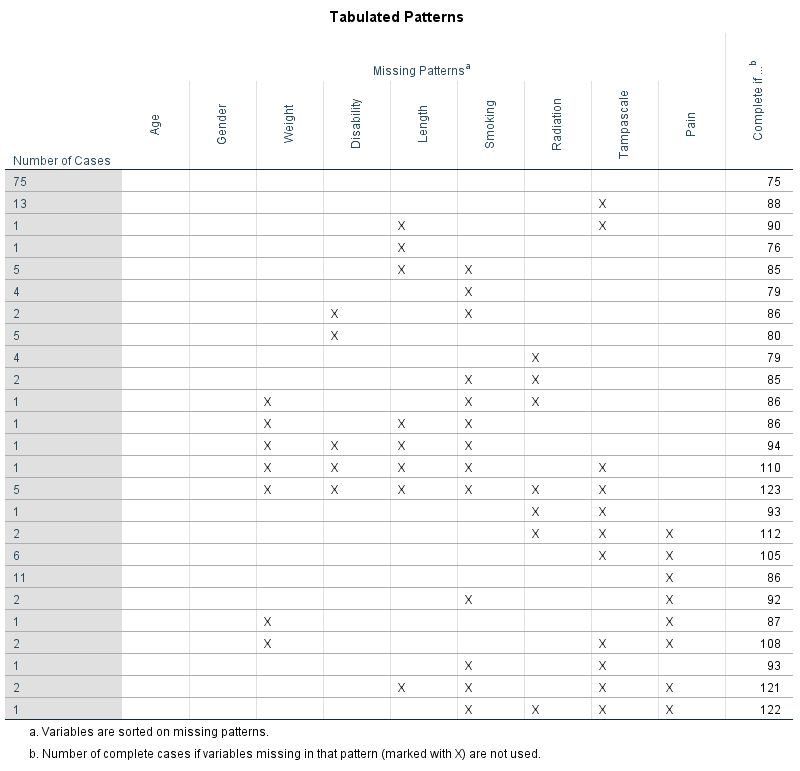
\includegraphics[width=0.9\linewidth]{images/tab2.1b} 

}

\caption{Descriptive missing data statistics and the missing data patterns.}\label{fig:tab2-1}
\end{figure}

Another way to obtain information about the missing data patterns is via
the Multiple Imputation option. To access this option, choose:
\textgreater{} Analyze -\textgreater{} Multiple Imputation
-\textgreater{} Analyze Patterns\ldots{}

\begin{figure}

{\centering 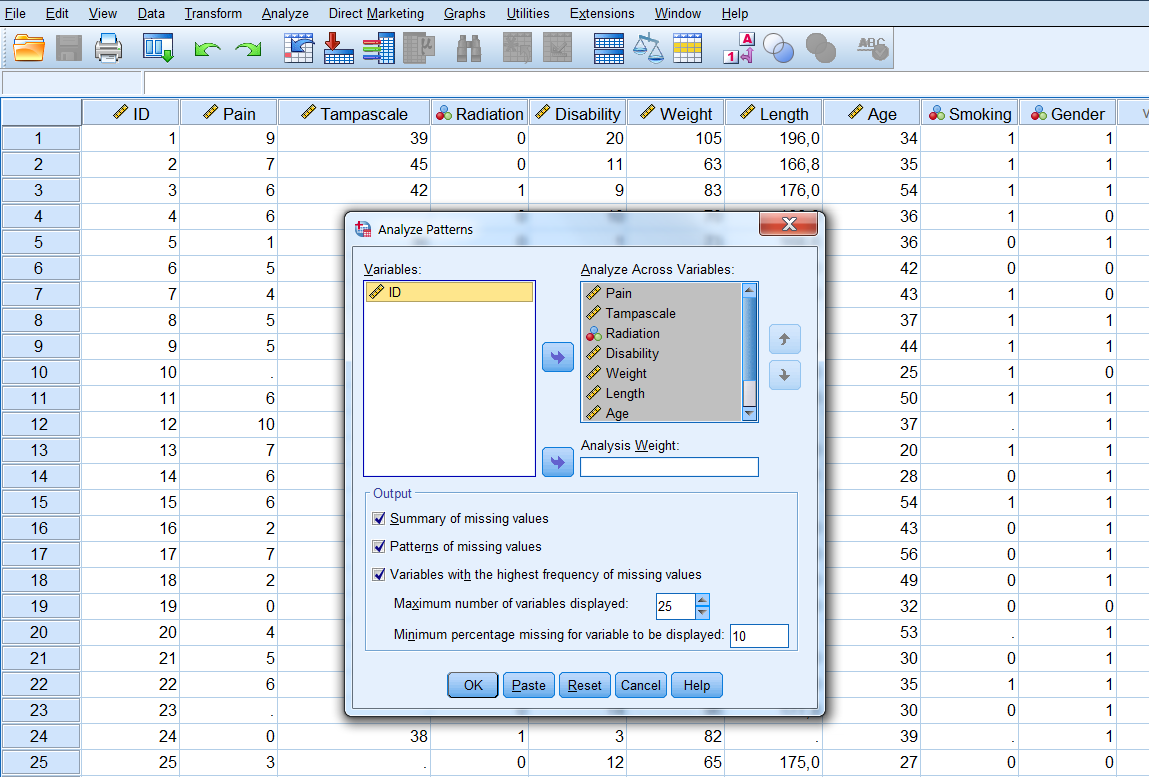
\includegraphics[width=0.9\linewidth]{images/fig2.5} 

}

\caption{Analyse Patterns menu.}\label{fig:fig2-5}
\end{figure}

Now transfer all variables that have to be analyzed for their missing
values to the window ``Analyze Across Variables''. We choose for the
following output options in that window:

Summary of missing values (displays missing data information in pie
charts, Patterns of missing values (displays tabulated patterns of
missing values) and Variables with the highest frequency of missing
values (displays a table of analysis variables sorted by percent of
missing values in decreasing order). To obtain the full list of all
patterns set the ``Minimum percentage missing for variable to be
displayed'' at 0. You can also adjust the maximum number of variables
displayed. This procedure will generate the following output:

\begin{figure}

{\centering 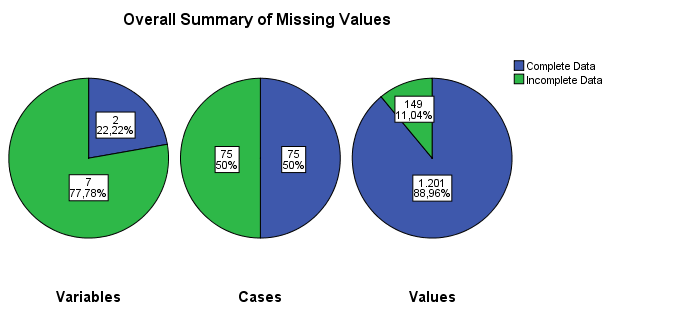
\includegraphics[width=0.9\linewidth]{images/fig2.6a} 

}

\caption{Output as a result of the Analyze Patterns menu under Multiple Imputation.}\label{fig:fig2-6}
\end{figure}\begin{figure}

{\centering 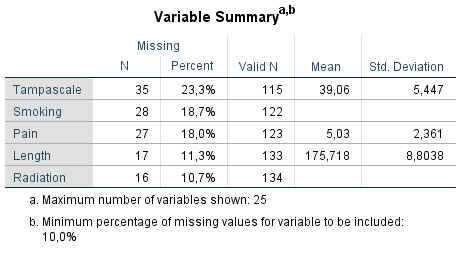
\includegraphics[width=0.9\linewidth]{images/fig2.6b} 

}

\caption{Output as a result of the Analyze Patterns menu under Multiple Imputation.}\label{fig:fig2-6}
\end{figure}\begin{figure}

{\centering 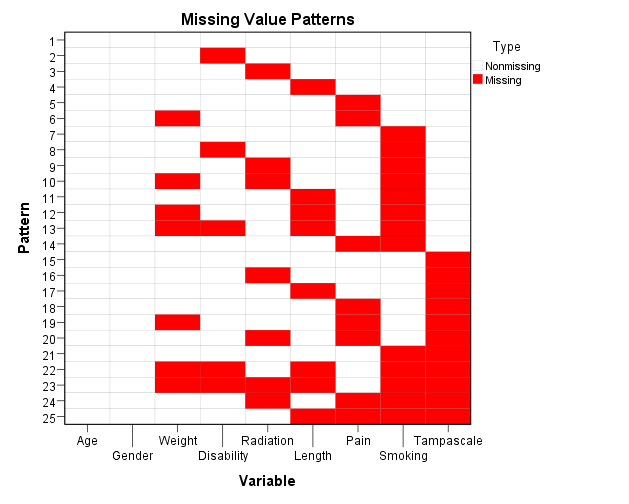
\includegraphics[width=0.9\linewidth]{images/fig2.6c} 

}

\caption{Output as a result of the Analyze Patterns menu under Multiple Imputation.}\label{fig:fig2-6}
\end{figure}\begin{figure}

{\centering 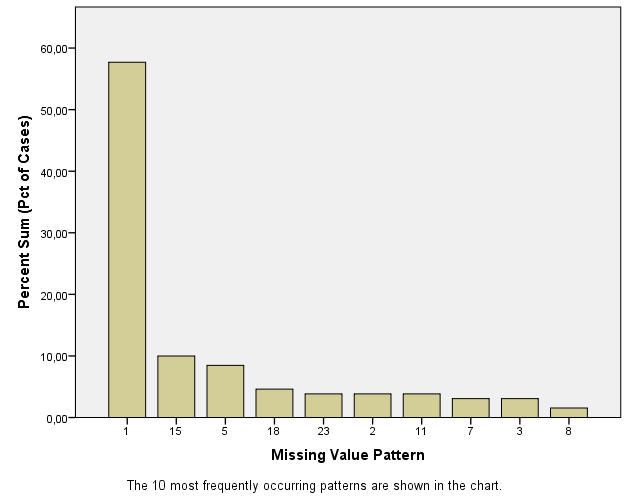
\includegraphics[width=0.9\linewidth]{images/fig2.6d} 

}

\caption{Output as a result of the Analyze Patterns menu under Multiple Imputation.}\label{fig:fig2-6}
\end{figure}

Summary of missing values (displays missing data information in pie
charts, Patterns of missing values (displays tabulated patterns of
missing values) and Variables with the highest frequency of missing
values (displays a table of analysis variables sorted by percent of
missing values in decreasing order). To get the full list of all
patterns set the ``Minimum percentage missing for variable to be
displayed'' at 0. You can also adjust the maximum number of variables
displayed. This procedure will generate the following output.

\subsection{Missing data patterns in
R}\label{missing-data-patterns-in-r}

To generate the missing data patterns in R we can make use of the mice
and \texttt{VIM} packages. We start with the \texttt{mice} package. That
package contains the \texttt{md.pattern} function that can generate the
missing data pattern.

\begin{Shaded}
\begin{Highlighting}[]
\KeywordTok{library}\NormalTok{(mice)}
\end{Highlighting}
\end{Shaded}

\begin{verbatim}
## Loading required package: lattice
\end{verbatim}

\begin{verbatim}
## 
## Attaching package: 'mice'
\end{verbatim}

\begin{verbatim}
## The following objects are masked from 'package:base':
## 
##     cbind, rbind
\end{verbatim}

\begin{Shaded}
\begin{Highlighting}[]
\KeywordTok{md.pattern}\NormalTok{(dataset)}
\end{Highlighting}
\end{Shaded}

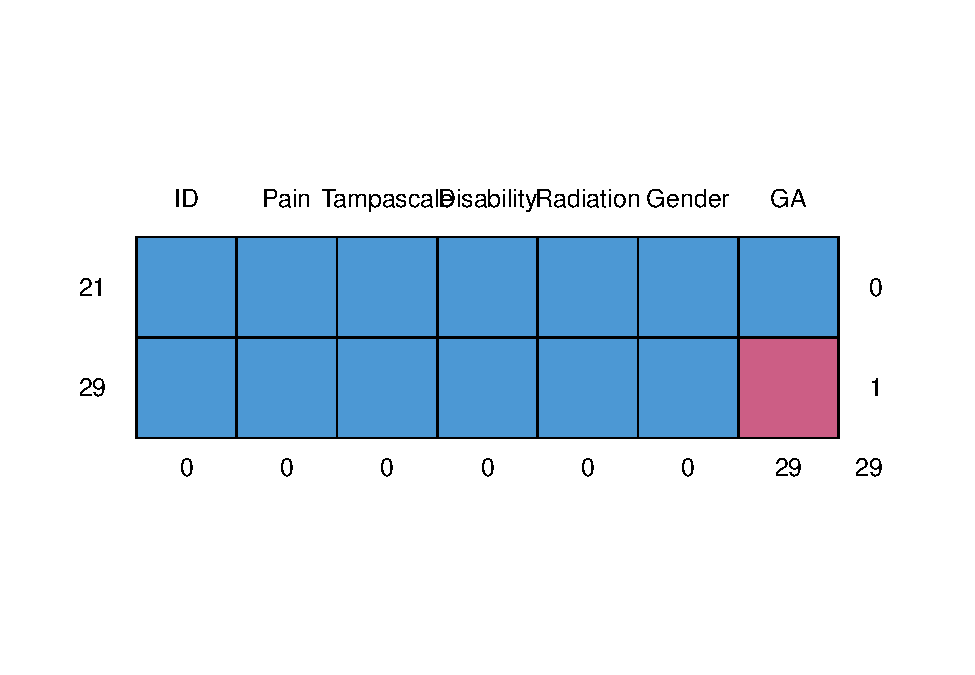
\includegraphics{Book_MI_files/figure-latex/unnamed-chunk-55-1.pdf}

\begin{verbatim}
##    ID Pain Tampascale Disability Radiation Gender GA   
## 21  1    1          1          1         1      1  1  0
## 29  1    1          1          1         1      1  0  1
##     0    0          0          0         0      0 29 29
\end{verbatim}

The first row contains the variable names. Each other row represents a
missing data pattern. The 1's in each row indicate that the variable is
complete and the 0's indicate that the variable in that pattern contains
missing values. The first column on the left (without a column name)
shows the number of cases with a specific pattern and the column on the
right shows the number of variables that is incomplete in that pattern.
The last row shows the total number of missing values for each variable.

To obtain a visual impression of the missing data patterns in R we use
the \texttt{VIM} package. That package contains the function
\texttt{aggr} As a result of using this function, the univariate
proportion of missing data is given in the Console window together with
two graphs.

\begin{Shaded}
\begin{Highlighting}[]
\KeywordTok{library}\NormalTok{(VIM)}
\end{Highlighting}
\end{Shaded}

\begin{verbatim}
## Loading required package: colorspace
\end{verbatim}

\begin{verbatim}
## Loading required package: grid
\end{verbatim}

\begin{verbatim}
## Loading required package: data.table
\end{verbatim}

\begin{verbatim}
## VIM is ready to use. 
##  Since version 4.0.0 the GUI is in its own package VIMGUI.
## 
##           Please use the package to use the new (and old) GUI.
\end{verbatim}

\begin{verbatim}
## Suggestions and bug-reports can be submitted at: https://github.com/alexkowa/VIM/issues
\end{verbatim}

\begin{verbatim}
## 
## Attaching package: 'VIM'
\end{verbatim}

\begin{verbatim}
## The following object is masked from 'package:datasets':
## 
##     sleep
\end{verbatim}

\begin{Shaded}
\begin{Highlighting}[]
\KeywordTok{aggr}\NormalTok{(dataset, }\DataTypeTok{col=}\KeywordTok{c}\NormalTok{(}\StringTok{'white'}\NormalTok{,}\StringTok{'red'}\NormalTok{), }\DataTypeTok{numbers=}\OtherTok{TRUE}\NormalTok{, }\DataTypeTok{sortVars=}\OtherTok{TRUE}\NormalTok{, }\DataTypeTok{cex.axis=}\NormalTok{.}\DecValTok{7}\NormalTok{, }\DataTypeTok{gap=}\DecValTok{3}\NormalTok{, }\DataTypeTok{ylab=}\KeywordTok{c}\NormalTok{(}\StringTok{"Percentage of missing data"}\NormalTok{,}\StringTok{"Missing Data Pattern"}\NormalTok{))}
\end{Highlighting}
\end{Shaded}

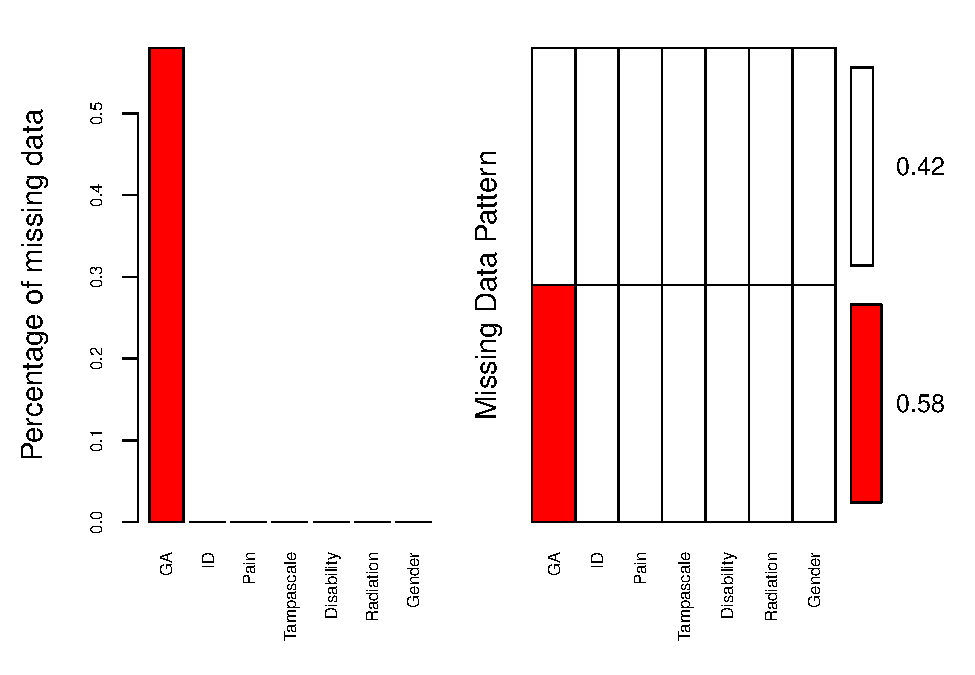
\includegraphics{Book_MI_files/figure-latex/unnamed-chunk-56-1.pdf}

\begin{verbatim}
## 
##  Variables sorted by number of missings: 
##    Variable Count
##          GA  0.58
##          ID  0.00
##        Pain  0.00
##  Tampascale  0.00
##  Disability  0.00
##   Radiation  0.00
##      Gender  0.00
\end{verbatim}

A histogram is displayed with the univariate percentage of missing
values in each variable, which is also shown as output in the Console
window and the patterns of missing data are also displayed. At the right
side of Figure 2.8 the proportion of patterns is presented. The variable
names are shown at the bottom of the figures. The red cells in the
Missing data patterns figure indicate that those variables contain
missing values. We see that 0.500 or 50\% of the patterns do not contain
missing values in any of the variables. Of the total patterns, 8.67\% of
the patterns have missing values in only the Tampa scale variable.

\section{2.3 Missing data Mechanisms}\label{missing-data-mechanisms}

By evaluating the missing data patterns, we can get insight in the
location of the missing data. With respect to the missing data mechanism
we are interested in the underlying reasons for the missing values and
the relationships between variables with and without missing data. In
general, we can say that missing values are either random or non-random.
Random missing values may occur because subjects accidentally do not
answer some questions or information of an entire subject is
accidentally not assessed. For example, a study subject has to fill out
some questionnaire instruments, gets distracted and misses a question
accidently or a questionnaire gets lost in the mail. Non-random missing
values may occur because subjects purposefully do not answer questions.
For example, subjects may be reluctant to answer questions about
sensitive topics like income, past crimes or sexual history. Rubin
introduced in 1976 a typology for missing data that makes a distinction
between random and non-random missing data situations, which are
abbreviated as MCAR, MAR and MNAR. These types of missing data are still
used as the basic missing data mechanisms. The key idea behind Rubin's
missing data mechanisms is that the probability of missing data in a
variable may or may not be related to the values of other measured
variables in the dataset. This means that we assume that there is some
kind of probability model for the missing data. With probability we
loosely mean the likelihood of a missing value to occur, i.e.~if a
variable has a lot of missing data, the probability of missing data in
that variable is high. This probability (i.e.~likelihood) can be related
to other measured or not-measured variables. For example, when mostly
older people have missing values, the probability for missing data is
related to age. Moreover, the missing data mechanisms also assume a
certain relationship (or correlation) between observed and variables
with missing values in the dataset. The extend of the relation between
observed variables and the probability of missing data, distinguishes
the three missing data mechanisms. In essence the missing data
mechanisms describe relationships between variables that may or may not
be causal, because in most missing data situations we never know the
real reason why data is missing. We will discuss the missing data
mechanisms in more detail below. As an example, we will use a study on
Low Back Pain (LBP). It is known that people with LBP may develop a fear
of movement (which is assessed by the Tampa scale) due to their pain in
the back. The idea is that these people believe that some underlying
serious problem causes their back pain and in order to prevent for more
damage they are afraid to move their back and experience a high fear of
movement.

\subsection{2.3.1 Missing Completely At
Random}\label{missing-completely-at-random}

Data are Missing Completely At Random (MCAR) when the probability that a
value is missing, is unrelated to the value of other observed (or
unobserved) variables, and unrelated to values of the missing data
variable itself. We will discuss what is means by using the LBP study as
an example. If LBP patients had to come to a research center to fill in
the Tampa scale (fear of movement) questionnaire and supply other
information for the study and some patients were not able to come
because they were ill that day due to the flu. In case of MCAR, there is
no relationship between having the flu and scores on the Tampa scale or
other study-related variables. This is realistic because there is no
evidence that patients with the flu, fear their back problem more, or
that the odds of having the flu is related to the study. For that
reason, we can assume that the missing data are MCAR. In other words,
the probability of missing data is not related to the values of the
Tampa scale variable. Another example is when respondents accidentally
skip questions in a questionnaire. Than the observed values of that
questionnaire are just a random sample of the entire dataset. An MCAR
missing data situation for the Tampa scale variable is visualized in the
MCAR column in the figure below. Although in real live we actually do
not know the completely observed data, as an example (for educational
reasons), the MCAR column is a copy of the completely observed Tampa
scale variable, with some values removed. When we compare the MCAR data
with the complete Tampa scale variable scores, we can observe that in
the MCAR situation an equal number of lower and higher values of the
Tampa scale variable are missing (in total 4 Tampa scores are missing, 2
for lower and 2 for higher values,). Also, the missing data in the Tampa
scale do not seem to be related to another variable like pain; an equal
number of Tampa scale values is missing for patients with low pain
scores as well as for patients with higher pain scores. This means that
the (observed) probability of missing data in the Tampa scale variable
will be equally large for lower and higher values of the Tampa scale and
of other measured variables in the data (i.e.~pain).

\begin{figure}

{\centering 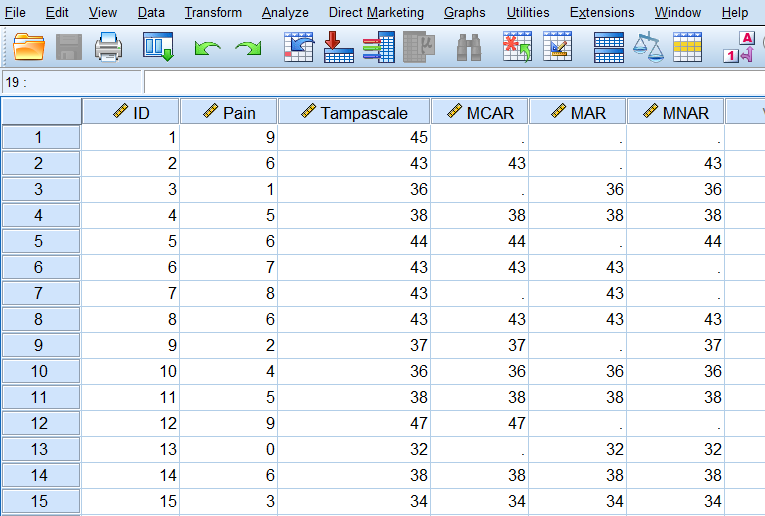
\includegraphics[width=0.9\linewidth]{images/fig2.7} 

}

\caption{Examples of MCAR, MAR and MNAR data.}\label{fig:fig2-7}
\end{figure}

This phenomenon for the Tampa scale variable in the LBP study is shown
in Figure \ref@(fig:tab2-2) below. This shows that the percentages (or
observed probabilities) of missing data are equally large for lower,
middle and higher values of the Tampa scale variable. These values are
presented as Percentile Groups of Tampa scale values with a range of
28-34, 35-37, 38-40, 41-44, 45-50 respectively. Over the whole range,
the percentage of missing data is around 25\% (equally large for
different values and (not shown) this is also the case for lower and
higher values of other variables e.g.~pain). In general, The MCAR
mechanism does not lead to parameter estimation problems as for example
invalid mean or regression coefficient estimates. However, excluding
cases with MCAR data will result in a smaller dataset for the analysis
and thus larger standard errors (i.e.~lower power).

\begin{figure}

{\centering 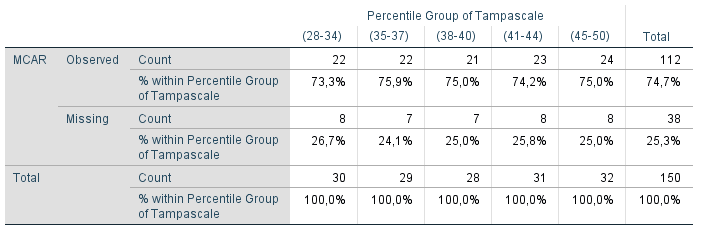
\includegraphics[width=0.9\linewidth]{images/tab2.2} 

}

\caption{MCAR missing data in the Tampa scale variable.}\label{fig:tab2-2}
\end{figure}

\subsection{Missing At Random}\label{missing-at-random}

The data are Missing At Random (MAR) when the probability that a value
for a variable is missing is related to other observed values in the
dataset but not to the variable itself. The reason of missing data may
lie outside the dataset but observed variables in the dataset capture
this by their associations. An example of MAR data is presented in the
MAR column of Figure \ref{fig:fig2-7} and Figure \ref{fig:tab2-3} for
150 LBP patients. In Figure \ref{fig:fig2-7} you can see in the MAR
column that 4 Tampa scale scores are missing for pain scores that are
\textgreater{} 5 and 1 for a pain score \textless{} 6, in other words
the probability of missing data in the Tampa scale scores is higher for
higher pain scores. In other words, patients with higher pain scores
(\textgreater{} 5) have more missing values on the Tampa scale variable
than patients with lower pain scores (\textless{} 6). However, within
the category of pain scores with values \textgreater{} 5, the Tampa
scale scores are MCAR, because within each category Tampa scale scores
are randomly missing for lower and higher values. In \ref{fig:tab2-3}
the Tampa scale data is split for at lower and higher pain score
categories. It can be observed that the means and standard deviations do
not differ between the observed and missing data for the Tampa scale
variable. Which is an indication that the Tampa scale data are MAR. (for
educational purposes we know the values of the missing values). A reason
could be that patients with higher Tampa scale scores were less likely
to show up at a next Tampa scale measurement because their back hurted
more. In a MAR missing data situation, missing values can be explained
by other (observed) variables, like for the Tampa scale and Pain
variable in the example above, due to the their (statistical)
relationship in the dataset. Further, within categories of the pain
variable (for low and high pain values) the Tampa scale scores are MCAR
(Raghunathan, 2016). However, it is not possible to test this
assumption, because for that you need information of the missing values
and that is impossible. In general, excluding MAR data leads to false
estimates of your statistical tests, like for example, regression
coefficients. A missing data method that works well with MAR data is
Multiple Imputation (Chapter 4).

\begin{figure}

{\centering 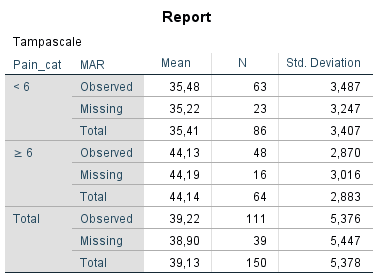
\includegraphics[width=0.9\linewidth]{images/tab2.3} 

}

\caption{MAR missing data in the Tampa scale variable.}\label{fig:tab2-3}
\end{figure}

\subsection{Missing Not At Random}\label{missing-not-at-random}

The data are MNAR when the probability of missing data in a variable is
related to the scores of that variable itself, e.g.~only high or low
scores are missing, and this missing data problem cannot be captured
anymore by other measured variables in the dataset because they are not
available in the dataset. In case of the LBP example, MNAR data occurs
when patients with the highest scores on the Tampa scale have missing
values. This is shown in the MNAR column of Figure \ref{fig:fig2-7}. The
MNAR column shows that the values that are most frequently missing are
the highest Tampa scale scores, i.e.~for the patients that fear their
back problems most. A reason may be that these patients were so afraid
to move (which is assessed by the Tamp scale), that they were not able
to visit an assessment center. MNAR missing data can also occur
indirectly through the relationship of the variable with missing data
with another variable that is not available in the dataset. For example,
it could also be that patients that worry the most do not want to be
confronted with questions about their fear to move their back and
therefore skip questions of the Tampa scale. In case of a positive
relationship between worriedness and fear of movement, the highest
values on the Tampa scale variable will be missing for those patients
that worry the most. If worriedness is not measured in the dataset, the
missing data in the Tampa scale variable will be MNAR. The difference
with MAR is that with MNAR, the missing data problem cannot be handled
by the observed variables in the dataset or by using a technique as
Multiple Imputation. However, as with MAR data, MNAR data can also not
be verified.

\subsection{The Missing Data
Indicator}\label{the-missing-data-indicator}

In the definitions of the missing data mechanisms in the previous
paragraphs we used the term probability several times, to indicate that
the relationship of variables with the probability of missingness in a
variable distinguishes the missing data mechanisms. The probability of
missing data can depend on other variables (MAR), on values of the
variables itself (MNAR) or not on other variables or values of the
variable itself (MCAR). Rubin (1987) proposed that variables with
missing data can be divided in a part that is observed and a part that
is missing. The observed and missing data can be coded by a 0 and 1
respectively. In case of the Tampa scale variable this means that the
observed data is coded by a 0 and a 1 is used for the Tampa scale values
that are missing. This dichotomous coding variable is called the missing
data indicator or R variable which means that the complete and missing
data are defined according to this variable. Figure \ref{fig:fig2-8}
shows the R indicator variable for the observed and missing data in the
Tampa scale variable. The R variable is now a single variable because
there is missing data in only the Tampa scale variable. When more
variables contain missing data, the R variable becomes a dataset of
variables that consist of 0´s and 1´s.

\begin{figure}

{\centering 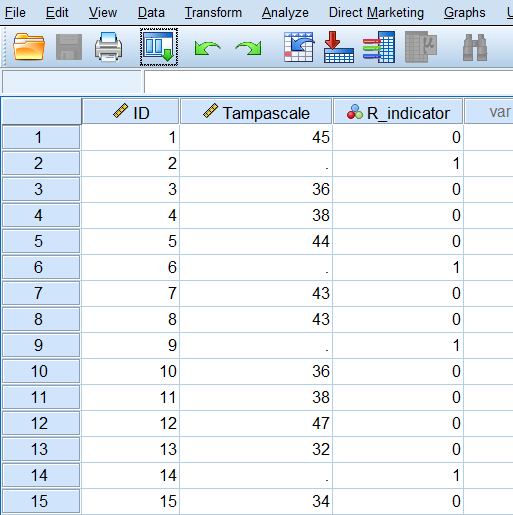
\includegraphics[width=0.9\linewidth]{images/fig2.8} 

}

\caption{The missing data in the Tampa scale variable coded according to the missing data indicator variable R.}\label{fig:fig2-8}
\end{figure}

Using the R indicator variable implies that missing values (or the
probability of missing values) can be described by a missing data model.
This missing data model may consist of variables that have a
relationship with the probability of missing data, in this case the R
indicator variable. A good example would be to use a logistic regression
model to describe the relationship of variables with the probability of
missing data in the Tampa scale variable. Graphically these models can
be visualized as in Figure 2.11. With logistic regression, which is in
essence a probability model, the relationship of a dichotomous outcome
variable (i.e.~the R missing data indicator variable) with other
variables can be described by using the models that are shown in Figure
2.12. In this Figure the missing data indicator variable R of the Tampa
scale variable that contain missing values is the outcome variable.

\begin{figure}

{\centering 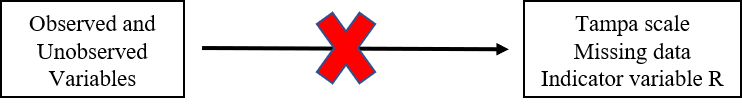
\includegraphics[width=0.9\linewidth]{images/fig2.9a} 

}

\caption{MCAR}\label{fig:fig2-9a}
\end{figure}

There is no relationship between, how the data became missing (indicated
by R) and observed and unobserved variables.

\begin{figure}

{\centering 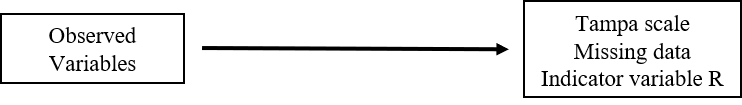
\includegraphics[width=0.9\linewidth]{images/fig2.9b} 

}

\caption{MAR}\label{fig:fig2-9b}
\end{figure}

There is a relationship between, how the data became missing (indicated
by R) and observed variables.

\begin{figure}

{\centering 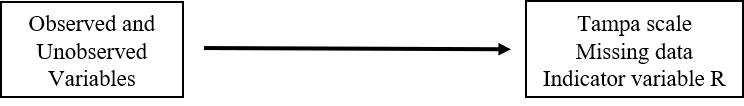
\includegraphics[width=0.9\linewidth]{images/fig2.9c} 

}

\caption{MNAR}\label{fig:fig2-9c}
\end{figure}

There is a relationship between, how the data got missing (indicated by
R) and observed and unobserved variables.

The missing data mechanisms of Rubin can then be described by the
following logistic regression models:

MCAR: No variables in or outside the dataset explain the missingness in
the Tampa scale variable, the model would be empty:
\[LN(\frac{R_{Tampa=1}}{1-R_{Tampa=1}}) = \beta_0\]

MAR: Variables in the dataset, like Pain and Radiation in the Leg
explain the missingness in the Tampa scale variable and the model would
be:
\[LN(\frac{R_{Tampa=1}}{1-R_{Tampa=1}}) = \beta_0 + \beta_1 * Pain +\beta_2 * Radiation\]

MNAR: Missingness in the Tampa scale variable can be explained by
variables in the dataset and by the score on the Tampa scale itself:

\[LN(\frac{R_{Tampa=1}}{1-R_{Tampa=1}}) = \beta_0 + \beta_1 * Pain + \beta_2 * Radiation + \beta_3 * Tampa\]

From these models we observe that the missing data models can be defined
by other observed variables in the dataset and/or missing data (which we
do not observe). It should be noted however, that we can never be
completely sure about the reason why data are missing. The above
mentioned relationships are therefore statistical relationships from
descriptive models and not from causal models.

In summary, the MCAR assumption is mostly very strict and not realistic
in practice.The MAR assumption is more realistic and mostly assumed in
practice.The difference bewteen MAR and MNAR is that in MNAR the
probability of missingness is also related to the unobserved (missing)
data.

\subsection{The Role of Auxiliary
Variables}\label{the-role-of-auxiliary-variables}

Usually, the probability of missing data is related to other variables
and/or to the missing values itself (MAR or MNAR). Unfortunately, it is
not possible to distinguish between MAR and MNAR mechanisms, because the
missing values are unknown. Brand (Brand, 1999) describes in Chapter 2
of his dissertation two examples that demonstrate how an initially MNAR
missing data mechanism can change into MAR by including additional
variables that are related to the probability of missing data. In
practice, by including variables related to the probability of missing
data a MNAR mechanism can get closer to a MAR mechanism. Accordingly,
the MAR assumption can be made more plausible by including additional
information in the missing data handling method (Baraldi \& Enders,
2010). Therefore, it is advised, to include extra variables that have a
relationship with the missing data rate in other variables, i.e.~have a
relationship with the probability of missing data or that have a
relationship (correlated) with the variables that contain the missing
values (Collins, 2001, Curran, Bacchi, Schmitz, Molenberghs, \&
Sylvester, 1998). These variables are called auxiliary variables and are
included in the imputation procedure to generate valid imputations.
These variables may not be required for further data analyses. In
general, the MCAR assumption is unrealistic and does not hold in most
datasets. As a practical solution, many studies assume a MAR mechanism.
Mostly, this mechanism is realistic, however it is advised to evaluate
the plausibility of this assumption in analyses explained below.

\section{Missing Data evaluation}\label{missing-data-evaluation-1}

A useful data evaluation and data imputation method depends on the
underlying missing data mechanism that is assumed. We have seen in
Paragraph 2.3 that the difference between the MCAR and not MCAR
mechanisms depend on the relationship of the missing data with the
observed variables. If this relationship cannot be detected by the
observed data in the dataset we assume that the data is MCAR. If there
is some kind of relationship, the missing data may be MAR or MNAR. We
can never distinct between MAR or MNAR data, because for that we need
information about the missing values and we do not have that
information. Tests to distinguish the missing data assumptions are
therefore only aimed to accept or reject the MCAR missing data
assumption. The MCAR assumption is mostly a too strict assumption to use
in practice because there is commonly some kind of reason why persons do
not fill in ``working'' questions. Moreover, in practice we study and
measure outcome and independent variables that are related to each
other. This makes that the MAR assumption is the most accepted
``working'' missing data assumption in practice. There are two ways to
evaluate the missing data mechanism. First, it is important to think
about the most plausible substantive reasons for the data being missing.
Researchers mostly have some possible explanation about why data are
missing and this information is very important. For example, when during
web based data collection, the internet sometimes disconnects because of
malfunction at the address of the internet provider, data of a few
participants gets lost. When these malfunctions are coincidental, it can
be assumed that the missing data are MCAR. However, when cognitive
scores are assessed during this web based data collection and these are
mostly not filled out by people that have decreased cognitive functions,
the missing data can be assumed to be MNAR. There are statistical test
procedures that can be used to get an idea about the missing data
mechanism. In these statistical tests, the non-responders (i.e.,
participants with missing observations), can be compared to the
responders on several characteristics. By doing this, we can test
whether the missing data mechanism is likely to be MCAR or not-MCAR
(because we cannot distinguish between MAR and MNAR missing data). There
are several possibilities to compare the non-responders with the
responders groups, for example using t-tests, a logistic regression with
a missing data indicator as the outcome, or Little's MCAR test (Little,
1988). To discuss these tests, we will use the example data from the
previous chapter, where we have measured several variables in a group of
150 low back pain patients and some variables contain missing
observations. In the examples below we will assume a MAR missing data
mechanism for the variables Tampa scale and Disability. Researchers need
to be aware that the assumptions that underlie an independent t-test,
logistic regression, and Chi-square test apply to these missing data
mechanism procedures as well. This means that the data is assumed to be
normally distributed and that the tests depend on a decent sample size.

\subsection{Missing data Evaluation in
SPSS}\label{missing-data-evaluation-in-spss}

\subsubsection{Descriptive Statistics}\label{descriptive-statistics}

Descriptive information of variables can be obtained via the following
options of the Missing Value Analysis (MVA) module in the SPSS menu:

\begin{quote}
Analyze -\textgreater{} Missing Value Analysis\ldots{}
\end{quote}

Transfer all variables in the correct Quantitative and Categorical
variables window and then click

\begin{quote}
Descriptives option -\textgreater{} Univariate statistics.
\end{quote}

\begin{figure}

{\centering 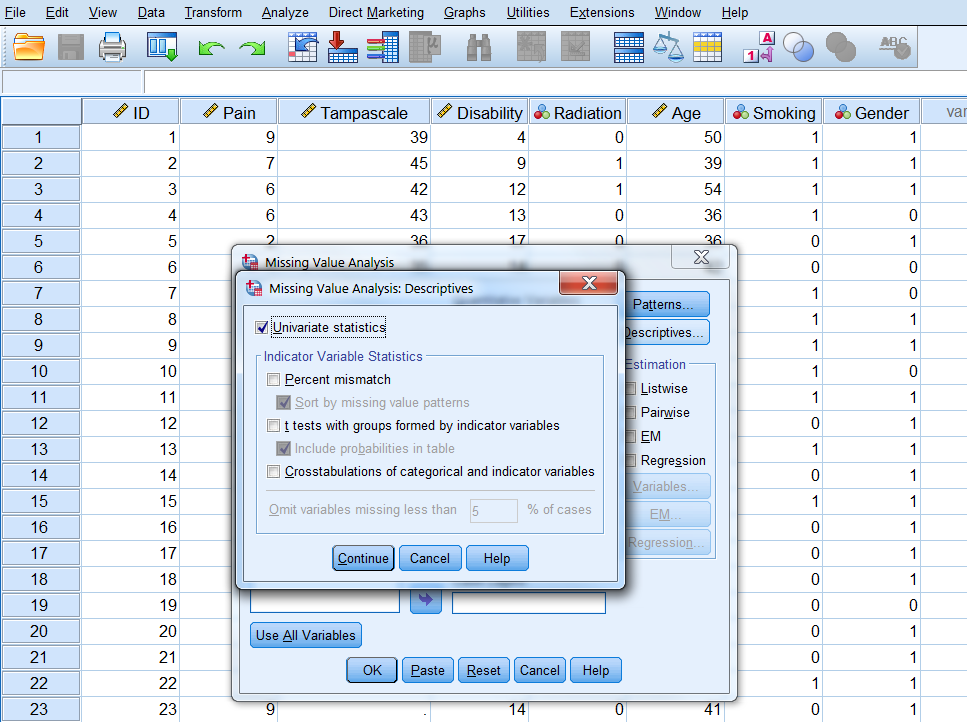
\includegraphics[width=0.9\linewidth]{images/fig2.10} 

}

\caption{Missing value Analysis menu in SPSS}\label{fig:fig2-10}
\end{figure}

\begin{figure}

{\centering 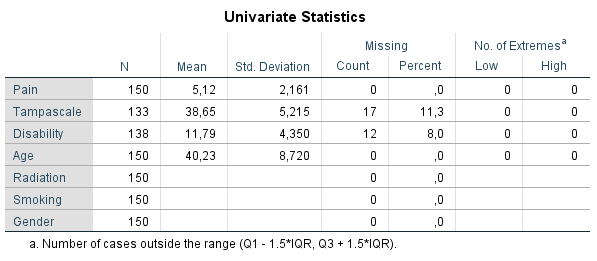
\includegraphics[width=0.9\linewidth]{images/tab2.4} 

}

\caption{Univariate descriptive statistics of variables with and without missing data.}\label{fig:tab2-4}
\end{figure}

Under the column N, the information of all cases in the dataset are
displayed, under the column Missing we get the number and percentage of
missing values in each variable and under the column No. of Extremes we
get information of cases that fall outside a range, which is specified
under the table. Further, for all continuous variables information about
the Mean and Standard deviation are displayed. No descriptive
information is given for categorical variables.

These descriptive information of variables with missing data gives us a
quick overview of the amount of missing data in each variable. However,
it does not provide us information about the relationship between
variables with complete and missing data and therefore does not give us
an idea about the potential missing data mechanism. Methods as T-tests,
regression or Little's MCAR test, that will be discussed in the next
section, can better be used for that purpose.

\subsubsection{T-test procedure}\label{t-test-procedure}

When we use the t-test procedure, SPSS first creates an indicator
variable, to distinguish the cases with missing values from the cases
with values that are present in each variable with missing values. Then,
group means are estimated and compared for other variables that are
complete with groups formed by the indicator variable, using Student's t
test. As a result, the t-statistic, degrees of freedom, counts of
missing and non-missing values, and means of the two groups are
displayed. You can also display any two-tailed probabilities associated
with the t statistic.

The t-test procedure can be found in: \textgreater{}Analyze
-\textgreater{} Missing Value Analysis\ldots{} -\textgreater{}
Descriptives -\textgreater{} click ``t-tests with groups formed by
indicator variables'' and ``include probabilities in table''
-\textgreater{} Continue -\textgreater{} OK.

\begin{figure}

{\centering 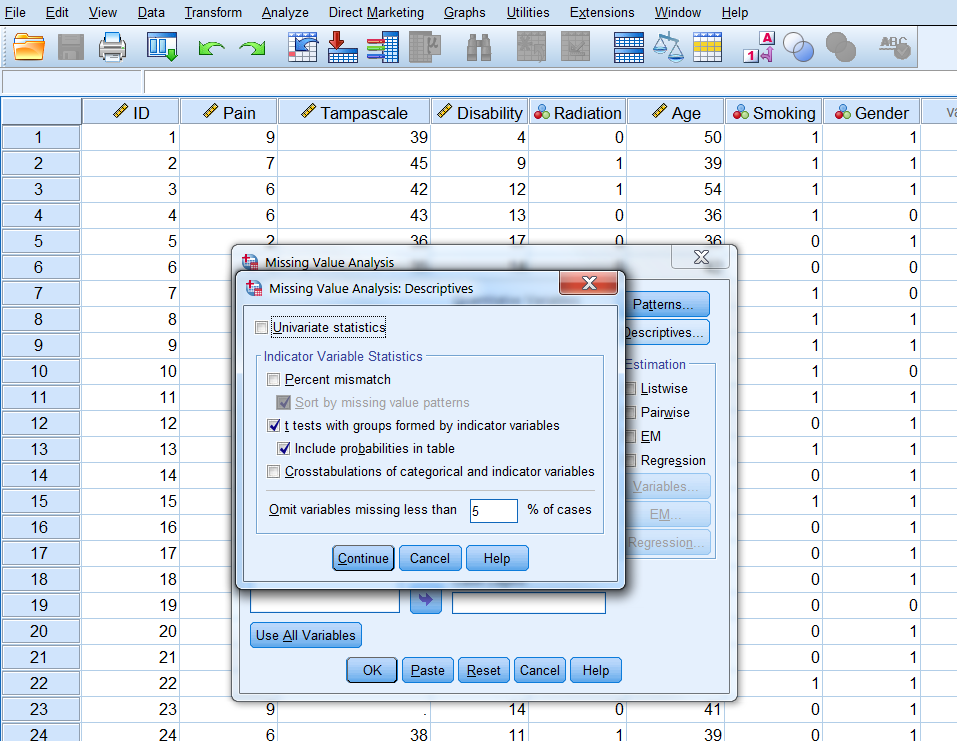
\includegraphics[width=0.9\linewidth]{images/fig2.11} 

}

\caption{The T-test procedure as part of the Missing Value Analysis menu}\label{fig:fig2-11}
\end{figure}

\begin{figure}

{\centering \includegraphics[width=0.9\linewidth]{images/tab2.5} 

}

\caption{Output table of the t-test procedure.}\label{fig:tab2-5}
\end{figure}

On the left side oft the output table the names of the variables with
missing values are presented which are the Tampa scale and Disability
variables. Of these variables, indicator variables are defined which are
used to compare group means of other variables, that can be tested for
significance using independent t-tests. The results of these t-tests are
given in the table according to the information in separate rows on the
left side with the t-value (t), degrees of freedom (df), P-value
(P(2-tail)), numbers of observed and missing cases (Present and Missing)
and means of observed and missing cases (Mean(Present) and
Mean(Missing)) presented. The variables for which the indicator groups
are compared, are listed in the columns of the table and are the Pain,
Tampa scale, Disability and Age variables. For the Tampa scale variable
that contain missing values, only the observed mean is presented,
because for the missing cases the values are missing! Notice that in the
row of the Tampa scale variable the means of the Disability variable can
still be compared between the observed and missing cases, because they
do not miss values for exactly the same cases. Table 2.5 shows that
patients that have observed values on the Tampa scale variable (row
Mean(Present)) differ significantly from patients with missing values on
the Tampa scale variable (row Mean(Missing)) on Pain (P(2-tail = 0.033)
and Disability (P(2-tail = 0.039). When we look at the means of the Pain
variable, we see that the mean of patients with missing values on the
Tampa scale variable is higher compared to the mean of patients with
observed scores. This means that there is a higher probability of
missing data on the Tampa scale variable for patients with higher pain
scores. If Tampa scale and Pain scores are correlated, the missing
values on the Tampa scale variable can also be explained by the Pain
score variable. This is also the case for the Age variable, but now the
t-test is not significant. For the Disability variable, it is the other
way around. We see more missing data on the Tampa scale variable for
lower Disability scores.

In the Missing Value Analysis window under the Indicator Variable
Statistics options you can also choose for ``Crosstabulations of
categorical and indicator variables''. In that case a separate table is
displayed for each categorical variable with missing values. For each
category of the variable, the frequency and percentages of non-missing
values for the other variables is displayed as well as the percentages
of each type of missing value. To reduce the size of the table, you can
omit statistics that are computed for only a small number of cases by
adjusting the option ``Omit variables missing less than \% of cases''.

\subsubsection{Logistic Regression
Analysis}\label{logistic-regression-analysis}

The missing data mechanism can also be evaluated with a logistic
regression procedure (Ridout, Society, \& Diggle, 1991). In the logistic
regression analysis, we can evaluate if the probability of missing data
is related to other variables in the data. For this procedure, we first
generate an indicator variable that separates the subjects with missing
values from the participants with observed values. This indicator
variable is used as the dependent variable in a logistic regression
analysis. A backward regression can be used to determine the strongest
predictors of missing data. The output for the logistic regression with
the Tampa scale variable as the indicator outcome variable is presented
below:

\begin{figure}

{\centering \includegraphics[width=0.9\linewidth]{images/tab2.6} 

}

\caption{Logistic regression analysis with variable that contain missing data as the outcome variable.}\label{fig:tab2-6}
\end{figure}

We can observe that the variable Pain is significantly related to the
missing data indicator variable of the Tampa scale variable, which
indicates that the probability for missing data in the Tampa scale
variable can be explained by the Pain variable. The positive coefficient
of 0.315 indicates that the probability of missing data on the Tampa
scale variable is higher for higher Pain scores. The other variables do
not show a significant relationship with missing data on the Tampa scale
variable. This logistic regression analysis procedure can be repeated
for each variable with missing values in the dataset.

\subsubsection{Little's MCAR test in
SPSS}\label{littles-mcar-test-in-spss}

Another possibility is to use a test that was developed by Roderick
Little: Little's MCAR test. This test is based on differences between
the observed and estimated mean in each missing data pattern. This test
is developed for continuous data. In this procedure, the missing data in
the whole dataset is evaluated, because each missing data pattern is
included in the analysis. To conduct this test, you choose from the SPSS
menu:

Analyze -\textgreater{} Missing Value Analysis\ldots{}In the main
Missing Value Analysis dialog box, select the variable(s) for which you
want to estimate missing values (use only continuous variables) and
Select EM in the Estimation group and Click OK.

\begin{figure}

{\centering \includegraphics[width=0.9\linewidth]{images/fig2.12} 

}

\caption{EM selection in the Missing Value Analysis menu.}\label{fig:fig2-12}
\end{figure}

\begin{figure}

{\centering \includegraphics[width=0.9\linewidth]{images/tab2.7a} 

}

\caption{Output tables with information of Little’s MCAR test.}\label{fig:tab2-7}
\end{figure}\begin{figure}

{\centering \includegraphics[width=0.9\linewidth]{images/tab2.7b} 

}

\caption{Output tables with information of Little’s MCAR test.}\label{fig:tab2-7}
\end{figure}\begin{figure}

{\centering \includegraphics[width=0.9\linewidth]{images/tab2.7c} 

}

\caption{Output tables with information of Little’s MCAR test.}\label{fig:tab2-7}
\end{figure}\begin{figure}

{\centering \includegraphics[width=0.9\linewidth]{images/tab2.7d} 

}

\caption{Output tables with information of Little’s MCAR test.}\label{fig:tab2-7}
\end{figure}\begin{figure}

{\centering \includegraphics[width=0.9\linewidth]{images/tab2.7e} 

}

\caption{Output tables with information of Little’s MCAR test.}\label{fig:tab2-7}
\end{figure}

\subsection{Missing data Evaluation in
R}\label{missing-data-evaluation-in-r}

\subsubsection{Little's MCAR test in R}\label{littles-mcar-test-in-r}

Little´s MCAR test is available in the \texttt{BaylorEdPsych} package
for R as the LittleMCAR function. To apply the test, we select only the
continuous variables. In the example blowe we use the dataset of 150 low
back pain patients with missing data in Genstatstional Age (GA). The
p-value for the test is not-siginificant, indicating that the missings
seem to be compeletely at random.

\begin{Shaded}
\begin{Highlighting}[]
\KeywordTok{library}\NormalTok{(BaylorEdPsych)}
\KeywordTok{LittleMCAR}\NormalTok{(dataset[,}\KeywordTok{c}\NormalTok{(}\StringTok{"Pain"}\NormalTok{, }\StringTok{"Tampascale"}\NormalTok{,}\StringTok{"Disability"}\NormalTok{, }\StringTok{"GA"}\NormalTok{)])}
\end{Highlighting}
\end{Shaded}

\begin{verbatim}
## Loading required package: mvnmle
\end{verbatim}

\begin{verbatim}
## this could take a while
\end{verbatim}

\begin{verbatim}
## $chi.square
## [1] 5.395246
## 
## $df
## [1] 3
## 
## $p.value
## [1] 0.14504
## 
## $missing.patterns
## [1] 2
## 
## $amount.missing
##                 Pain Tampascale Disability    GA
## Number Missing     0          0          0 29.00
## Percent Missing    0          0          0  0.58
## 
## $data
## $data$DataSet1
##    Pain Tampascale Disability GA
## 2     6         43         10 36
## 6     7         43         11 29
## 8     6         43         11 34
## 10    4         36          3 38
## 13    0         32          3 42
## 15    3         34         13 39
## 17    3         35         11 26
## 20    4         32          9 28
## 25    5         36          6 35
## 28    3         36          3 36
## 30    6         37         16 40
## 32    4         37          8 39
## 34    2         37          3 37
## 37    8         47          8 35
## 39    3         39          8 33
## 41    7         45         10 32
## 44    1         35          2 34
## 46    5         41         17 38
## 47    6         43         11 41
## 48    3         39          9 33
## 50    8         44         19 32
## 
## $data$DataSet2
##    Pain Tampascale Disability GA
## 1     9         45         20 NA
## 3     1         36          1 NA
## 4     5         38         14 NA
## 5     6         44         14 NA
## 7     8         43         18 NA
## 9     2         37         11 NA
## 11    5         38         16 NA
## 12    9         47         14 NA
## 14    6         38         12 NA
## 16    6         42          8 NA
## 18    1         31          1 NA
## 19    2         31          7 NA
## 21    5         39         13 NA
## 22    5         39         12 NA
## 23    4         34          8 NA
## 24    8         47         13 NA
## 26    5         38         16 NA
## 27    9         48         23 NA
## 29    2         36          9 NA
## 31   10         43         21 NA
## 33   10         42         20 NA
## 35    6         43         12 NA
## 36    3         38          7 NA
## 38    3         38          6 NA
## 40    7         44         15 NA
## 42    6         40         12 NA
## 43    7         40         16 NA
## 45    9         41         19 NA
## 49    2         33          6 NA
\end{verbatim}

\chapter{Single Missing data
imputations}\label{single-missing-data-imputations}

\section{Complete cases analysis}\label{complete-cases-analysis}

Complete case analysis (CCA) means that persons with a missing data
point in a variable are excluded from the analysis. This procedure is
still used a lot (Eekhout et al. 2012) but can have a large negative
impact on the precision of the statistical test results. It also leads
to an incorrect estimation of standard errors when the data is MCAR, MAR
and MNAR (Eekhout et al. 2014). It is for that reason generally not
recommended. It is however, the default procedure in a lot of
statistical software packages as in SPSS.

\section{Mean Imputation}\label{mean-imputation}

Assume that we are interested in the relationship between Pain and the
Tampa scale variable. To get a first impression about this relationship
we make a scatterplot. The scatterplots of the complete and incomplete
datasets are displayed in (Figure \ref{fig:fig3-1} and
\ref{fig:fig3-2}):

\begin{figure}

{\centering \includegraphics[width=0.9\linewidth]{images/fig3.2a} 

}

\caption{ Relationship between the Tampa scale and Pain variables (green dots are observed and red dots are assumed to be missing data}\label{fig:fig3-1}
\end{figure}

\begin{figure}

{\centering \includegraphics[width=0.9\linewidth]{images/fig3.2b} 

}

\caption{Relationship between the Tampa scale and Pain variable. Missing data are excluded}\label{fig:fig3-2}
\end{figure}

The green dots represent the observed data and the red dots the missing
data points. In practice, in your dataset you have the available points
that are visualized in Figure \ref{fig:fig3-2}.

\subsection{Mean imputation in SPSS}\label{mean-imputation-in-spss}

The easiest methods to do mean imputation are by using the \emph{Replace
Missing Values} procedure under Transform and by using the \emph{Linear
Regression} procedure.

\emph{Replace Missing Values procedure}

You can find the Replace Missing Values dialog box via

\begin{quote}
Transform -\textgreater{} Replace Missing Values.
\end{quote}

A new window opens. Transport the Tampa scale variable to the New
variable(s) window (Figure \ref{fig:fig3-3}). The default imputation
procedure is Mean imputation or called ``Series mean''.

\begin{figure}

{\centering \includegraphics[width=0.9\linewidth]{images/fig3.6} 

}

\caption{Window for mean imputation of the Tampa scale variable.}\label{fig:fig3-3}
\end{figure}

When you click on OK, a new variable is created in the dataset using the
existing variable name followed by an underscore and a sequential
number. The result is shown in Figure \ref{fig:fig3-7}.

\begin{figure}

{\centering \includegraphics[width=0.9\linewidth]{images/fig3.7} 

}

\caption{Mean imputation of the Tampa scale variable with the Replace Missing Values procedure.}\label{fig:fig3-7}
\end{figure}

The scatterplot between the Pain and the Tampa scale variable clearly
shows the result of the mean imputation procedure, all imputed values
are located at the mean value (Figure \ref{fig:fig3-4}).

\begin{figure}

{\centering \includegraphics[width=0.9\linewidth]{images/fig3.4} 

}

\caption{Scatterplot between the Tampa scale and Pain variable, after the missing values of the Tampa scale variable have been replaced by the mean.}\label{fig:fig3-4}
\end{figure}

\emph{Linear Regression}

Mean imputation in SPSS is also integrated in the Linear Regression menu
via:

\begin{quote}
Analyze -\textgreater{} Regression -\textgreater{} Linear
-\textgreater{} Options.
\end{quote}

In the Missing Values group you choose for Replace with mean (Figure
\ref{fig:fig3-8}).

\begin{figure}

{\centering \includegraphics[width=0.9\linewidth]{images/fig3.8} 

}

\caption{The option Replace with mean in the Linear Regression menu.}\label{fig:fig3-8}
\end{figure}

You can also obtain the mean values by using \emph{Descriptive
Statistics}, and than replace the missing values by using the recode
procedures:

\begin{quote}
Transform -\textgreater{} Recode into Same Variables.
\end{quote}

\subsection{Mean imputation in R}\label{mean-imputation-in-r}

You can do mean imputation by using the mice function in the mice
package.

\begin{Shaded}
\begin{Highlighting}[]
\KeywordTok{library}\NormalTok{(foreign) }\CommentTok{# activate the foreign package to use the read.spss function}
\NormalTok{dataset <-}\StringTok{ }\KeywordTok{read.spss}\NormalTok{(}\DataTypeTok{file=}\StringTok{"Backpain 50 missing.sav"}\NormalTok{, }\DataTypeTok{to.data.frame=}\NormalTok{T)}
\end{Highlighting}
\end{Shaded}

\begin{verbatim}
## re-encoding from UTF-8
\end{verbatim}

\begin{Shaded}
\begin{Highlighting}[]
\KeywordTok{library}\NormalTok{(mice) }\CommentTok{# Activate the mice package to use the mice function}
\NormalTok{imp_mean <-}\StringTok{ }\KeywordTok{mice}\NormalTok{(dataset, }\DataTypeTok{method=}\StringTok{"mean"}\NormalTok{, }\DataTypeTok{m=}\DecValTok{1}\NormalTok{, }\DataTypeTok{maxit=}\DecValTok{1}\NormalTok{)}
\end{Highlighting}
\end{Shaded}

\begin{verbatim}
## 
##  iter imp variable
##   1   1  Tampascale
\end{verbatim}

You can extract the mean imputed dataset by using the complete function.

\begin{Shaded}
\begin{Highlighting}[]
\KeywordTok{complete}\NormalTok{(imp_mean)}
\end{Highlighting}
\end{Shaded}

\section{Regression imputation}\label{regression-imputation}

\subsection{Regression imputation in
SPSS}\label{regression-imputation-in-spss}

Yoy do regression imputation in SPSS via the Missing Value Analysis
procedures. There are two options for regression imputation, the
Regression option and the EM (Expectation Maximization) option. The
Regression option in SPSS has some flaws in the estimation of the
regression parameters (see paper von Hippel 2004). Therefore, we use the
EM algorithm. This algorithm is a likelihood-based procedure. This means
that the most likely values of the regression coefficients are estimated
given the data and subsequently used to impute the missing value. This
EM procedure gives the same results as first performing a normal
regression analysis in the dataset and subsequently estimate the missing
values from the regression equation, after the missing values have been
excluded. We will compare the EM and regression procedures below.

\subsubsection{EM procedure}\label{em-procedure}

Step 1, Choose:

\begin{quote}
Analyze -\textgreater{} Missing Value Analysis\ldots{}
\end{quote}

In the main Missing Value Analysis dialog box, select the variable(s)
that you want to use for the regression method and select EM in the
Estimation group (Figure \ref{fig:fig3-10}).

\begin{figure}

{\centering \includegraphics[width=0.9\linewidth]{images/fig3.10} 

}

\caption{EM Selection in the Missing Value Analysis window.}\label{fig:fig3-10}
\end{figure}

Step 2 click Variables, to specify predicted and predictor variables.
Place the Tampascale variable in the window of the Predicted variables
and the Pain variable in the Predictor Variables window (Figure
\ref{fig:fig3-11}).

\begin{figure}

{\centering \includegraphics[width=0.9\linewidth]{images/fig3.11} 

}

\caption{Transfer of the Tampascale and Pain variables to the Predicted and Predictor Variables windows.}\label{fig:fig3-11}
\end{figure}

Step 3 Click on Continue -\textgreater{} EM and Choose for Normal in the
Distribution group. Than thick Save completed data and give the dataset
a name, for example ``ImpTampa\_EM'' (Figure \ref{fig:fig3-12}).

\begin{figure}

{\centering \includegraphics[width=0.9\linewidth]{images/fig3.12} 

}

\caption{Name of dataset to save the EM results in.}\label{fig:fig3-12}
\end{figure}

Step 4 Click Continue -\textgreater{} OK. The new dataset
``ImpTampa\_EM'' will open in a new window in SPSS. In this dataset the
imputed data of the Tampascale Variable together with the original data
is stored (Figure \ref{fig:fig3-13}, first 15 patients are shown).
Adjust the Width and Decimals of the Tampa scale variable in the
Variable View window to 4 and 3 respectively to get the same results as
in Figure 3.13.

\begin{figure}

{\centering \includegraphics[width=0.9\linewidth]{images/fig3.13} 

}

\caption{Result of the EM procedure.}\label{fig:fig3-13}
\end{figure}

Be aware that SPSS uses as default only quantitative variables to impute
the missing values with the EM algorithm. If you want to include
categorical variables in the imputation model as auxiliary variables,
you have to define them as scale variables.

\subsubsection{Normal Linear Regression}\label{normal-linear-regression}

We now compare the EM procedure with a two-step linear regression
procedure. We first estimate the relationship between Pain and the Tampa
scale variable in the dataset with linear regression after we have
excluded the cases with missing values in the Tampa scale variable.
Subsequently, we use the regression coefficients from this regression
model to estimate the imputed values in the Tampa scale variable. Start
by estimating the linear regression model with the Tampa scale variable
as outcome variable (because we have to predict missing values in this
variable) and use the Pain variable as the independent variable.

To estimate the linear regression model, choose:

\begin{quote}
Analyze -\textgreater{} Regression -\textgreater{} Linear
\end{quote}

Transfer the Tampa scale variable to the Dependent variable window and
the Pain variable to the window of the Block 1 of 1 group. Then click
OK.

\begin{figure}

{\centering \includegraphics[width=0.9\linewidth]{images/fig3.14} 

}

\caption{Linear regression analysis with the Tampa scale as the outcome and Pain as the independent variable.}\label{fig:fig3-14}
\end{figure}

The following coefficients will be estimated (Figure \ref{fig:tab3-3}).

\begin{figure}

{\centering \includegraphics[width=0.9\linewidth]{images/table3.3} 

}

\caption{Result of the linear regression analysis.}\label{fig:tab3-3}
\end{figure}

The linear regression model can be described as:

Tampascale=32.005+1.410 ×Pain

Now impute the missing values in the Tampa scale variable and compare
them with the EM estimates. You see that the results are the same.

\begin{figure}

{\centering \includegraphics[width=0.9\linewidth]{images/fig3.15} 

}

\caption{Predictions of the missing Tampa scale values on basis of the regression model estimated in the dataset after the missing values were excluded.}\label{fig:fig3-15}
\end{figure}

When you make a scatterplot of the imputations from the regression model
you see that, as expected, the imputed values lie directly on the
regression line (Figure \ref{fig:fig3-16}).

\begin{figure}

{\centering \includegraphics[width=0.9\linewidth]{images/fig3.16} 

}

\caption{Relationship between the Tampa scale and the Pain variable.}\label{fig:fig3-16}
\end{figure}

The Tampa scale variable is located on the y-axis. The imputed values of
the Tampa scale variable (red dots) are located on the regression line
that was used to generate the imputed values. The green dots are the
observed data values.

\subsection{Regression imputation in
R}\label{regression-imputation-in-r}

You can aplly regression imputation in R with as method ``norm.predict''
in the mice function. The Pain variable is used to predict the missing
values in the Tampa scale variable.

\begin{Shaded}
\begin{Highlighting}[]
\KeywordTok{library}\NormalTok{(foreign)}
\NormalTok{dataset <-}\StringTok{ }\KeywordTok{read.spss}\NormalTok{(}\DataTypeTok{file=}\StringTok{"Mean imputation.sav"}\NormalTok{, }\DataTypeTok{to.data.frame=}\NormalTok{T)}
\end{Highlighting}
\end{Shaded}

\begin{verbatim}
## re-encoding from UTF-8
\end{verbatim}

\begin{Shaded}
\begin{Highlighting}[]
\NormalTok{dataset <-}\StringTok{ }\NormalTok{dataset[, }\KeywordTok{c}\NormalTok{(}\StringTok{"Pain"}\NormalTok{, }\StringTok{"Tampascale"}\NormalTok{)]}

\NormalTok{imp.regress <-}\StringTok{ }\KeywordTok{mice}\NormalTok{(dataset, }\DataTypeTok{method=}\StringTok{"norm.predict"}\NormalTok{, }\DataTypeTok{m=}\DecValTok{1}\NormalTok{, }\DataTypeTok{maxit=}\DecValTok{1}\NormalTok{)}
\end{Highlighting}
\end{Shaded}

\begin{verbatim}
## 
##  iter imp variable
##   1   1  Tampascale
\end{verbatim}

\begin{Shaded}
\begin{Highlighting}[]
\NormalTok{imp.regress}\OperatorTok{$}\NormalTok{imp}\OperatorTok{$}\NormalTok{Tampascale }\CommentTok{# Extract the imputed values}
\end{Highlighting}
\end{Shaded}

\begin{verbatim}
##           1
## 2  40.46554
## 6  41.87566
## 9  34.82506
## 14 40.46554
## 21 39.05542
## 25 39.05542
## 27 44.69590
## 31 46.10602
## 35 40.46554
## 37 43.28578
## 44 33.41494
## 49 34.82506
## 50 43.28578
\end{verbatim}

Expectantly, this gives comparable results as the regression imputation
with SPSS above. The method ``norm.predict'' in the mice package fits a
linear regression model in the dataset after the missing data is
excluded and generates the imputed values for the Tampa scale variable
by using the regression coefficients of the linear regression model. The
same regression coefficients are used to predict the missing values in
the Tampa scale variable as shown in Table 3.3. The completed dataset
can be extracted by using the complete function in the mice package.

\subsection{Stochastic regression
imputation}\label{stochastic-regression-imputation}

With Stochastic regression models imputation uncertainty is accounted
for by adding extra error variance to the predicted values that are
generated by the linear regression model. Stochastic regression can be
activated in SPSS via the Missing Value Analysis and the Regression
Estimation option. However, the Regression Estimation option generates
incorrect regression coefficient estimates (von Hippel, 2004) and will
therefore not further discussed.

\subsection{Stochastic regression imputation in
R}\label{stochastic-regression-imputation-in-r}

You can apply stochastic regression imputation in R with the mice
function. For this you use as method ``norm.nob''.

\begin{Shaded}
\begin{Highlighting}[]
\NormalTok{dataset <-}\StringTok{ }\KeywordTok{read.spss}\NormalTok{(}\DataTypeTok{file=}\StringTok{"Backpain 50 missing.sav"}\NormalTok{, }\DataTypeTok{to.data.frame=}\NormalTok{T)}
\end{Highlighting}
\end{Shaded}

\begin{verbatim}
## re-encoding from UTF-8
\end{verbatim}

\begin{Shaded}
\begin{Highlighting}[]
\NormalTok{dataset <-}\StringTok{ }\NormalTok{dataset[, }\KeywordTok{c}\NormalTok{(}\StringTok{"Pain"}\NormalTok{, }\StringTok{"Tampascale"}\NormalTok{)]}

\NormalTok{imp_nob <-}\StringTok{ }\KeywordTok{mice}\NormalTok{(dataset, }\DataTypeTok{method=}\StringTok{"norm.nob"}\NormalTok{, }\DataTypeTok{m=}\DecValTok{1}\NormalTok{, }\DataTypeTok{maxit=}\DecValTok{1}\NormalTok{)}
\end{Highlighting}
\end{Shaded}

\begin{verbatim}
## 
##  iter imp variable
##   1   1  Tampascale
\end{verbatim}

The completed dataset can be extracted by using the complete function in
the mice package.

\section{Bayesian Stochastic regression
imputation}\label{bayesian-stochastic-regression-imputation}

The difference between the non-Bayesian imputation procedure that you
applied above and Bayesian imputation is that with the latter method
extra variation is added to the imputed values via the regression
coefficients. The idea is used that there is not one true (population)
regression coefficient but that the regression coefficient itself
follows a (probability) distribution. This is in contrast to the
frequentist idea, which assume that there is one true population
parameter. In this case the regression coefficient (is reflected by the
confidence interval). In this book (and most statistial books) the
freuentist approach is used For more information about the theory of
Bayesian statistics we refer to the books of Box and Tiao (1992), Enders
(2012) and Gelman et al. (2004).

\subsection{Bayesian Stochastic regression imputation in
SPSS}\label{bayesian-stochastic-regression-imputation-in-spss}

In SPSS Bayesian Stochastic regression imputation can be performed via
the multiple imputation menu. To generate imputations for the Tampa
scale variable, we use the Pain variable as the only predictor.

Step 1

To start the imputation procedure, Go to

\begin{quote}
Analyze -\textgreater{} Multiple Imputation -\textgreater{} Impute
Missing Data Values.
\end{quote}

In the first window you define which variables are included in the
imputation model. Transfer the Tampa scale and Pain variable to the
Variables in Model window. Than set the number of imputed datasets to 1
under Imputations and give the dataset where the imputed values are
stored under ``Create a new dataset'' a name. Here we give it the name
``ImpStoch\_Tampa'' (Figure \ref{fig:fig3-18}).

\begin{figure}

{\centering \includegraphics[width=0.9\linewidth]{images/fig3.18} 

}

\caption{The Variables window.}\label{fig:fig3-18}
\end{figure}

Step 2

In the Methods window, choose under Imputation Method for customand then
Fully conditional specification (MCMC). Set the Maximum iterations
number at 50. This specifies the number of iterations as part of the FCS
method (Figure \ref{fig:fig3-19}). We further use the default settings.

\begin{figure}

{\centering \includegraphics[width=0.9\linewidth]{images/fig3.19} 

}

\caption{The Methods window.}\label{fig:fig3-19}
\end{figure}

Step 3

In the constraints window (Figure \ref{fig:fig3-20}) click on the Scan
Data button and further use the default settings.

\begin{figure}

{\centering \includegraphics[width=0.9\linewidth]{images/fig3.20} 

}

\caption{Stochastic regression imputation}\label{fig:fig3-20}
\end{figure}

Step 4

In the Output window we only use the default settings.

\begin{figure}

{\centering \includegraphics[width=0.9\linewidth]{images/fig3.21} 

}

\caption{The Output window.}\label{fig:fig3-21}
\end{figure}

Step 5

Now click on OK button to start the imputation procedure

The output dataset consists of the original data with missing data plus
a set of cases with imputed values for each imputation. These imputed
datasets are stacked under each other. The file also contains a new
variable, Imputation\_, which indicates the number of the imputed
dataset (0 for original data and more than 0 for the imputed datasets).
The variable Imputation\_ is added to the dataset and the imputed values
are marked yellow.

\begin{figure}

{\centering \includegraphics[width=0.8\linewidth]{images/fig3.22} 

}

\caption{Aanpassen Titel.}\label{fig:fig3-22}
\end{figure}

\begin{figure}

{\centering \includegraphics[width=0.8\linewidth]{images/fig3.23} 

}

\caption{Imputed dataset with the imputed values marked yellow.}\label{fig:fig3-23}
\end{figure}

When we make a scatterplot of the Pain and the Tampascale variable
(Figure \ref{fig:fig3-24}) we see that there is more variation in the
Tampascale variable, or you could say that the variation in the
Tampascale variable is ``repaired''.

\begin{figure}

{\centering \includegraphics[width=0.9\linewidth]{images/fig3.24} 

}

\caption{Scatterplot of the relationship between Tampascale and the Pain variable, including the imputed values for the Tampascale variable (red dots).}\label{fig:fig3-24}
\end{figure}

The full Multiple Imputation procedure will be discussed in more detail
in the next Chapter.

\subsection{Bayesian Stochastic regression imputation in
R}\label{bayesian-stochastic-regression-imputation-in-r}

The package mice also include a Bayesian stochastic regression
imputation procedure. This method also accounts for imputation
uncertainty, not only via the residuals (error variance), but also via
the regression coefficients, which means that extra noise (or random
error) is added to the regression coefficients. This imputation
procedure is done by using the mice.impute.norm function. For the
example to apply this method in R code 3.8 we use the same dataset as
above with missing values in the Tampa scale variable and the pain
variable as the only predictor variable for these missing values.

\begin{Shaded}
\begin{Highlighting}[]
\NormalTok{dataset <-}\StringTok{ }\KeywordTok{read.spss}\NormalTok{(}\DataTypeTok{file=}\StringTok{"Backpain 50 missing.sav"}\NormalTok{, }\DataTypeTok{to.data.frame=}\NormalTok{T)}
\end{Highlighting}
\end{Shaded}

\begin{verbatim}
## re-encoding from UTF-8
\end{verbatim}

\begin{Shaded}
\begin{Highlighting}[]
\NormalTok{dataset <-}\StringTok{ }\NormalTok{dataset[, }\KeywordTok{c}\NormalTok{(}\StringTok{"Pain"}\NormalTok{, }\StringTok{"Tampascale"}\NormalTok{)]}

\NormalTok{imp_b <-}\StringTok{ }\KeywordTok{mice}\NormalTok{(dataset, }\DataTypeTok{method=}\StringTok{"norm"}\NormalTok{, }\DataTypeTok{m=}\DecValTok{1}\NormalTok{, }\DataTypeTok{maxit=}\DecValTok{1}\NormalTok{)}
\end{Highlighting}
\end{Shaded}

\begin{verbatim}
## 
##  iter imp variable
##   1   1  Tampascale
\end{verbatim}

\begin{Shaded}
\begin{Highlighting}[]
\NormalTok{imp_b}\OperatorTok{$}\NormalTok{imp}\OperatorTok{$}\NormalTok{Tampascale }\CommentTok{# Extract the imputed values}
\end{Highlighting}
\end{Shaded}

\begin{verbatim}
##           1
## 2  39.56653
## 6  40.26110
## 9  36.92183
## 14 38.45535
## 21 45.59280
## 25 42.32326
## 27 42.29989
## 31 47.33560
## 35 39.33439
## 37 43.95467
## 44 34.28893
## 49 38.02693
## 50 46.41343
\end{verbatim}

The completed dataset can be extracted by using the complete function in
the mice package.

Predictive Mean Matching: Predictive mean matching (PMM) is an
imputation method that predicts values and subsequently selects observed
values to be used to replace the missing values. It is the default
imputation procedure in the mice package to impute missing data in
continuous variables (Rubin, 1987, p.~168). The strength of this
procedure is that missing data is replaced by data that is observed in
the dataset and not replaced by unrealistic values (as negative body
weight values).

\chapter{Data analysis after Multiple
Imputation}\label{data-analysis-after-multiple-imputation}

In the previous Chapter we discussed multiple imputation (MI) and how
imputations in multiple datasets are generated. After the imputations
have been generated, the data analysis and pooling steps follow. This
chapter explains these steps. In the data analysis step, the statistical
model is applied in the imputed datasets. In the pooling step, the
analysis results from the analysis step, are summarized into one final
result. The biggest challenge is to summarize the statistical results
into one estimate with the related pooled standard errors, confidence
intervals and a pooled p-value. Rubin (1987) provided rules which can be
applied to many different statistical tests. Rubin's rules are not
available for all statistical procedures in SPSS. Many test procedures
that do not have pooling results not available in SPSS are available in
R. We will start this Chapter with an example of applying t-tests in
multiple imputed datasets. With this procedure we can explain the use of
Rubin's Rules (RR), and the derivation of the degrees of freedom for
hypothesis testing, which can become complex. We will further discuss
missing data measures that are derived from RR, such as the fraction of
missing information (FMI), the relative increase in variance due to
missing data (Relative Increase Variance) and Relative Efficiency. We
will further show other pooling procedures for frequently used
statistical techniques and how to apply them in multiply imputed
datasets. The availability of each method in SPSS and R, are discussed
and their application is presented. Specific pooling methods that are
not available in SPSS are discussed by using examples in R.

\section{Rubin's Rules - A first
example}\label{rubins-rules---a-first-example}

Rubin proposed methods to combine statistical test results into one
(pooled) summary estimate. These so-called Rubin´s Rules (RR) are
designed to pool parameter estimates, such as means differences and
regression coefficients, standard errors and to derive confidence
intervals and p-values. T-tests are frequently used and suitable to
discuss all aspects of using RR, from pooling parameter estimates to
deriving degrees of freedom and p-values. We will first illustrate the
use of RR with a t-test example in 3 generated multiple imputed datasets
in SPSS. In this example we will pool the mean differences and standard
errors. The derivation of the test statistic t for hypothesis testing,
degrees of freedom and p-value may differ between the statistical method
used. These derivations are explained but also discussed in more detail.
As an illustration, we use de LBP study again, and test the Tampascale
mean difference (dependent variable) between backpain patients with and
without radiation in the leg (dependent variable). The output of the
t-test in the multiple imputed data can be found in (Figure
\ref{fig:tab5-1a}).

\begin{figure}

{\centering \includegraphics[width=0.9\linewidth]{images/table5.1} 

}

\caption{T-test for difference in mean Tampascale values between patients with and without Radiation in the leg applied in multiple imputed datasets.}\label{fig:tab5-1a}
\end{figure}

\begin{figure}

{\centering \includegraphics[width=0.9\linewidth]{images/table5.1b} 

}

\caption{b.T-test for difference in mean Tampascale values between patients with and without Radiation in the leg applied in multiple imputed datasets.}\label{fig:tab5-1b}
\end{figure}

In (Figure \ref{fig:tab5-1a}) the relationship in the original dataset
is presented in the row that is indicated by Imputation\_ number 0 as
well as in each imputed dataset which are indicated by Imputation\_
number 1 to 3. In the last row which is indicated as ``Pooled'', the
summary estimates of the parameters are presented. With parameters we
mean the parameters of interest which are here the mean differences and
standard errors. We will explain now by using RR how these pooled mean
differences and standard errors are estimated.

\subsection{Pooling Parameters}\label{pooling-parameters}

When RR are used, it is assumed that the repeated parameter estimates in
each imputed dataset (e.g.~mean differences), are normally distributed.
This cannot be assumed for all statistical test statistics,
e.g.~correlation coefficients. For these test statistics,
transformations have to be performed before RR can be applied to assume
normality (will be discussed below). To illustrate the use of RR, we
start with the T-test example of (Figure \ref{fig:tab5-1a})

To calculate the pooled parameter estimate the following formula is used
\eqref{eq:p-param}:

\begin{equation}
  \bar{\theta} = \frac{1}{m}\left (\sum_{i=1}^m{\theta_i}\right )
  \label{eq:p-param}
\end{equation}

In this formula, \(\bar{\theta}\) is the pooled parameter estimate, m is
the number of imputed datasets, \(\theta_i\) means taking the sum of the
parameter estimate (i.e.~mean difference) in each imputed dataset i.
This formula is equal to the basic formula of taking the mean value of a
sequence of numbers.

When we use the values in (Figure \ref{fig:tab5-1a}), \(\theta_i\) is
the mean difference of the Tampascale variable between patients with and
without radiation in the leg in each imputed dataset, we get the
following result:

\[\bar{\theta} = \frac{1}{3}(2.174 + 1.965+1.774)=1.971\]

This value of 1.971 is the pooled value for the Tampascale variable in
(Figure \ref{fig:tab5-1a}).

\section{Pooling Standard errors}\label{pooling-standard-errors}

The pooled standard error is derived from different components that
reflect the within and between sampling variance of the parameter of
interest. To calculate the within and between sampling variance in the
t-test example, the mean difference and the related standard errors are
needed. The calculation of these components is discussed below.

\emph{Within imputation variance} The within imputation variance is the
average of the variance of the estimates in each imputed dataset. This
reflects the sampling variance, i.e.~the precision of the parameter of
interest in each completed dataset. This value will be large in small
samples and small in large samples. The within imputation variance is
computed by taking the mean of the within variance estimate,
i.e.~squared standard error, in each imputed dataset:

\begin{equation}
V_W = \frac{1}{m}\left (\sum_{i=1}^m{SE_i^2}\right )
  \label{eq:var-w}
\end{equation}

In this formula \(V_W\) is the within imputation variance, m is the
number of imputed datasets, \(SE_i^2\) means taking the sum of the
squared Standard Error (SE), estimated in each imputed dataset i. Using
the data in (Figure \ref{fig:tab5-1a}), we get the following result:

\[V_W = \frac{1}{3}(0.896^2 + 0.882^2 + 0.898^2)=0.7957147\]

\emph{Between imputation variance} The between imputation variance
reflects the extra variance due to the missing data. This is estimated
by taking the variance of the parameter of interest estimated over
imputed datasets. This value is large when the level of missing data is
high and smaller when the level of missing data is small.

\begin{equation}
V_B\sqrt{\frac{\sum_{i=1}^m (\theta_i - \overline{\theta})^2}{N-1} }
  \label{eq:var-b}
\end{equation}

In this formula, \(V_B\) is the between imputation variance, m is the
number of imputed datasets, \(\overline{\theta}\) is the pooled
estimate, \(\theta_i\) is the parameter estimate in each imputed dataset
i. Accordingly, \({\sum_{i=1}^m(\theta_i - \overline{\theta})^2}\) ,
indicates taking the sum of the squared differences, between the
individual and pooled parameter estimates in each imputed dataset. This
formula is equal to the formula for the (sample) variance which is
commonly used in statistics. Using the data in (Figure
\ref{fig:tab5-1a}), we get the following result for the between
imputation variance:

\[V_W = \frac{1}{3-1}((2.174-1.971)^2+ (1.965-1.971)^2+(1.774-1.971)^2)=0.7957147\]

\[V_B = \frac{V_B}{m}\]

\begin{equation}
V_{Total} = V_W + V_B + \frac{V_B}{m}
  \label{eq:var-t}
\end{equation}

\[V_{Total} = 0.7957147+0.040027 + \frac{0.040027}{3}\]

\[SE_{Pooled} = \sqrt{V_{Total}} = \sqrt{0.849084} = 0.9214575\]

This value is equal to the (rounded) pooled standard error value of
0.921 in (Figure \ref{fig:tab5-1a}).

\section{Significance testing}\label{significance-testing}

For significance testing of the pooled parameter, i.e.~the mean
difference in (Figure \ref{fig:tab5-1a}), Formula 5.6 is used. This is
the univariate Wald test (Rubin 1987, van Buuren 2013, Marshall, 2009).
This test is defined as:

\begin{equation}
Wald_{Pooled} =\frac{(\overline{\theta} - {\theta_0})^2}{V_T}
  \label{eq:wald-pooled}
\end{equation}

where \(\overline{\theta}\) and \(V_T\) is the total variance and is
equal to the \(SE_P\) or the pooled standard error that was derived in
the previous paragraph), and \(\theta_0\) is the parameter value under
the null hypothesis (which is mostly 0). The univariate Wald test can be
used to test all kind of univariate parameters of interest, mean
differences and univariate regression coefficients in linear and
logistic regression models. In our example, we use the univariate Wald
test to test the pooled mean difference for significance. The univariate
Wald test in our example is calculated using the values from (Figure
\ref{fig:tab5-1a}):

\[Wald_{Pooled} =\frac{(\overline{\theta} - {\theta_0})^2}{V_T}=\frac{1.971}{\sqrt{0.849084}}=2.139\]
The univariate pooled Wald value follows a t-distribution. This
distribution is used to derive the p-value. The value for t depends on
the degrees of freedom, according to:

\begin{equation}
t_{df,1-\alpha/2}
  \label{eq:t-distr}
\end{equation}

Where df is degrees of freedom and \(\alpha\) is the reference level of
significance, which is usually set at 5\%. The derivation of the degrees
of freedom for the t-test is complex because there exist different
formula´s to calculate the degrees of freedom. This is explained in the
next paragraph.

Because \(t^2\) is equal to F at the same number of degrees of freedom,
we can also test for significance using a F-distribution, according to:

\begin{equation}
F_{1, df}=t^2_{df,1-\alpha/2}
  \label{eq:f-distr}
\end{equation}

The degrees of freedom are equal to the degrees of freedom for the
t-test above.

\section{Degrees of Freedom and
P-values}\label{degrees-of-freedom-and-p-values}

The derivation of the degrees of freedom (df) and the resulting p-value
for the pooled T-test is not straightforward, because there are
different formulas to calculate the df. There exists an older version of
the formula to calculate the degrees of freedom (df) and an adjusted
version (Van Buuren 2012). The older method to calculate the dfs results
in a higher df than those in each imputed dataset. An example of this is
shown in (Figure \ref{fig:tab5-2}). It can be seen that the degrees of
freedoms is 148 in each imputed dataset (in the row for equal variances
assumed) and 507 for the pooled result. Although this difference in df
may seem small, using different values for the degrees of freedom leads
to different p-values. In SPSS the old way to calculate the dfs is used.
Adjusted versions are used in the mice package for R. The differences
between the older and adjusted method to calculate the dfs is
illustrated below.

\begin{figure}

{\centering \includegraphics[width=0.9\linewidth]{images/table5.2} 

}

\caption{Part of Output of Figure 5.1. The value for the dfs are presented in the df column.}\label{fig:tab5-2}
\end{figure}

The (older method) to calculate df for the t-distribution is described
in Rubin (1987) and Van Buuren (2012) and is defined as:

\begin{equation}
df_{Old} = \frac{m-1}{lambda^2} = (m-1) * (1 + \frac{1}{r^2})
  \label{eq:df-old}
\end{equation}

Where m is the number of imputed datasets and lambda can be interpreted
as the Fraction of Missing information (FMI), calculated by Formula 5.13
(Raghunathan, 2016), and r is the relative increase in variance due to
nonresponse, calculated by Formula 5.14. The calculation of lambda and r
values are discussed in more detail below. The lambda value that is used
in Formula 5.9 (and often used as alternative for the FMI) is not the
same FMI value of 0.067 that SPSS presents in (Figure
\ref{fig:tab5-1a}). The FMI value of 0.067 is calculated by Formula 5.16
and is called FMI in this manual.

When \(df_{old}\) is calculated with the information in (Figure
\ref{fig:tab5-1a}), we get:

\[df_{Old} = \frac{3-1}{0.06283485^2} = 506.5576\]

This (rounded) value is equal to the df value in the row Pooled of 507
in (Figure \ref{fig:tab5-1a}). Formula 5.9 leads to a larger df for the
pooled result, compared to the dfs in each imputed dataset, which is
inappropriate. Therefore, Barnard and Rubin (1999) adjusted this df by
using Formula 5.10:

\begin{equation}
df_{Adjusted} = \frac{df_{Old}*{df_{Observed}}}{df_{Old}+{df_{Observed}}}
  \label{eq:df-adj}
\end{equation}

Where \(df_{Old}\) is defined as in Formula 5.9 and \(df_{Observed}\) is
defined as:

\begin{equation}
df_{Observed} = \frac{(n-k)+1}{(n-k)+3}*(n-k)(1-lambda)
  \label{eq:df-obs}
\end{equation}

Where n is the sample size in the imputed dataset, k the number of
parameters to fit and lambda is obtained by Formula 5.13.

By filling in the formulas 5.11 and 5.10 we get for \(df_{observed}\)
and \(df_{adjusted}\) respectively:

\[df_{Observed} = \frac{(150-2)+1}{(150-2)+3}*(150-2)(1- 0.06283485)=136.8633\]

\[df_{Adjusted} = \frac{(506.5576* 136.8633)}{(506.5576+ 136.8633)}=107.7509\]

This number of 107.7509 is equal to the df used by mice.

We can now derive the p-value for the mean difference in the Tampascale
between patients with and without Radiation in the leg. This two-sided
p-value is:

In SPSS:

\[t_{df,1-\alpha/2}=2.139_{df{Old}}=0.03289185\]

\[t_{df,1-\alpha/2}=2.139_{df{Adjusted}}=0.03467225\] \#\# Confidence
Intervals

For the 95\% confidence interval (CI), the general formula can be used:

\begin{equation}
\bar{\theta} ± t_{df,1-\alpha/2} * SE_{Pooled}
  \label{eq:conf}
\end{equation}

In this formula, \(\bar{\theta}\) is the pooled estimate, t is the
t-statistic, df is degrees of freedom and \(SE_{Pooled}\) is the pooled
standard error (Formula 5.5).

\section{Measures of Missing data
information}\label{measures-of-missing-data-information}

In this paragraph we will discuss measures that can be derived from
values of the between, and within imputation variance and the total
variance. These measures are the Fraction of Missing information (FMI),
the relative increase in variance due to nonresponse and the Relative
Efficiency. There exist two versions of the FMI, which are referred to
as lambda and FMI.

\subsection{Fraction of Missing
Information}\label{fraction-of-missing-information}

The Fraction of Missing information, lambda, (van Buuren, 2012;
Raghunathan, 2016) can be derived from the between and total missing
data variance as:

\begin{equation}
Lambda = \frac{V_B + \frac{V_B}{m}}{V_T}
  \label{eq:lambda}
\end{equation}

Where m is the number of imputed datasets and \({V_B}\) and \({V_T}\)
are the between and total variance respectively. This value can be
interpreted as the proportion of variation in the parameter of interest
due to the missing data.

When we use the \({V_B}\) and \({V_T}\) values that were calculated in
paragraph 5.1.2, this value will be:

\[Lambda = \frac{0.040027 + \frac{0.040027}{3}}{0.849084}=0.06283485\]

This specific value for the FMI, lambda, is not reported by SPSS, but is
reported by the mice package in R. Confusingly, van Buuren (2012) and
Enders (2010) use the same formula to calculate this type of missing
data information, but van Buuren calls it lambda and Enders FMI.

\subsection{Relative increase in
variance}\label{relative-increase-in-variance}

Another related measure is the relative increase in variance (RIV) due
to nonresponse. This value is calculated as:

\begin{equation}
Lambda = \frac{V_B + \frac{V_B}{m}}{V_W}
  \label{eq:riv}
\end{equation}

Where \({V_B}\) and \({V_W}\) are the between and within variance
respectively. This value can be interpreted as the proportional increase
in the sampling variance of the parameter of interest that is due to the
missing data.

Filling in this formula with the example from paragraph 5.1.2 will
result in:

\[Lambda = \frac{V_B + \frac{V_B}{m}}{V_W}=\frac{0.040027 + \frac{0.040027}{3}}{0.7957147}=0.06704779\]

This value is also presented in (Figure \ref{fig:tab5-1a}) in the column
Relative Increase Variance.

\subsection{Fraction of Missing Information -
FMI}\label{fraction-of-missing-information---fmi}

\begin{equation}
FMI = \frac{RIV + \frac{2}{df+3}}{1+RIV}
  \label{eq:riv}
\end{equation}

Where RIV is the relative increase in variance due to missing data (see
Formula 5.14) and df is the degrees of freedom for the pooled result.
The degrees of freedom for the pooled result can be obtained in two
ways: df\_Old or df\_Adjusted.

In SPSS, FMI is calculated using df\_Old, which results in:

\[FMI = \frac{RIV + \frac{2}{df+3}}{1+RIV}=\frac{0.06704779 + \frac{2}{506.5576+3}}{1+0.06704779}=0.0665132\]

In R package mice, FMI is calculated using the formula for df\_Adjusted,
that results in:

\[FMI = \frac{RIV + \frac{2}{df_{Adjusted}+3}}{1+RIV}=\frac{0.06704779 + \frac{2}{107.7509+3}}{1+0.06704779}=0.0797587\]

The difference between lambda and FMI is that FMI is adjusted for the
fact that the number of imputed datasets that are generated is not
unlimitedly large. These measures differ for a small value of the df.

\subsection{Relative Efficiency}\label{relative-efficiency}

The Relative Efficiency (RE) is defined as:

\begin{equation}
RE = \frac{1}{1+\frac{FMI}{m}}
  \label{eq:re}
\end{equation}

FMI is the fraction of missing information and m is the number of
imputed datasets.

The RE value is only provided by SPSS and is calculated by filling in
the values of (Figure \ref{fig:tab5-1a}) as follows:

\[RE = \frac{1}{1+\frac{FMI}{m}}=\frac{1}{1+\frac{0.0665132}{3}}=0.9783098\]

The RE gives information about the precision of the parameter estimate
as the standard error of a regression coefficient.

\section{Pooling Data Analytic results after MI in SPSS and
R}\label{pooling-data-analytic-results-after-mi-in-spss-and-r}

In Chapter 4 we discuss that when multiple imputation is applied, the
multiple imputed datasets can be stored in a separate SPSS file. In
order to obtain pooled analysis results in SPSS, the imputed values must
be marked yellow (i.e.~the file should be split by the Imputation\_
variable). See (Figure \ref{fig:tab5-1a}) for an example of a multiple
imputed dataset with imputed values marked yellow.

\begin{figure}

{\centering \includegraphics[width=0.9\linewidth]{images/fig5.1} 

}

\caption{Example of SPSS dataset after MI has been applied.}\label{fig:fig5-1}
\end{figure}

If SPSS does not recognize the dataset as a multiple imputed dataset,
the data will be treated as one large dataset, which is wrong. Marking
the values can be done by using the option ``Mark Imputed Data'' under
the View menu in the Data View window ((Figure \ref{fig:fig5-1})). The
Imputation\_ variable is a nominal variable that separates the original
from the imputed datasets. It is used as a variable that splits the file
into separate groups for analysis based on the different categories.
This is also indicated in the corner on the right side below in the Data
View and Variable View windows by the remark ``Split by imputation\_''.

\begin{figure}

{\centering \includegraphics[width=0.9\linewidth]{images/fig5.2} 

}

\caption{Procedure to mark imputed values in SPSS.}\label{fig:fig5-2}
\end{figure}

When imputation markings are turned on, a special icon is displayed next
to procedures that support pooling after multiple imputation ((Figure
\ref{fig:fig5-3})).

\begin{figure}

{\centering \includegraphics[width=0.05\linewidth]{images/fig5.3} 

}

\caption{Multiple Imputation icon.}\label{fig:fig5-3}
\end{figure}

This icon is shown in the analyze menu in SPSS ((Figure
\ref{fig:fig5-4a}) and (Figure \ref{fig:fig5-4b})). In (Figure
\ref{fig:fig5-4b}) the imputed values are not marked. SPSS assumes that
the dataset is just a normal dataset and the special icon is not visible
when you use Analyze \textgreater{} Regression. When the imputed values
are marked as in (Figure \ref{fig:fig5-4b}), the special icon appears
again.

\begin{figure}

{\centering \includegraphics[width=0.9\linewidth]{images/fig5.4a} 

}

\caption{The dataset is not recognized as an imputed dataset (no special icon visible).}\label{fig:fig5-4a}
\end{figure}

\begin{figure}

{\centering \includegraphics[width=0.9\linewidth]{images/fig5.4b} 

}

\caption{The dataset is recognized as an imputed dataset (special icon visible).}\label{fig:fig5-4b}
\end{figure}

In Appendix C a list of SPSS procedures is presented that support
multiple imputed datasets. SPSS provides two levels of pooling, which
are called the Naïve and Univariate combination. The Naïve combination
only shows the pooled parameter (if available). The Univariate
combination shows the pooled parameter, its standard error, test
statistic, effective degrees of freedom, p-value, confidence interval,
and pooling diagnostics (fraction of missing information, relative
efficiency, relative increase in variance), when available. Although the
special icon in SPSS to indicate that the dataset is recognized as a
multiple imputed dataset appears for many analysis procedures, it is not
always clear what procedures also provide the Univariate combination
output. It is therefore recommended to explore what kind of pooled
information is provided by SPSS before MI is applied. The mice package
is considered the main package in this manual to APPLY multiple
imputation in R. Many pooling procedures are available in the mice
package. However, for some specific statistical procedures, other
packages are required to obtain pooled estimates. For example, pooling
ANOVA results is not available in the mice package itself, the miceadds
package has to be used for that by using the function mi.anova. The
consequence is that if you are planning to do an ANOVA analysis in
multiply imputed datasets you may have to use the mice and the miceadds
packages. For a complete list of available procedures in different R
packages see Appendix D. In this chapter we will provide pooled results
in SPSS and R. In other words, we will show results of statistical
procedures for which pooled information is available. As an example we
use a dataset for 150 patients with Back pain. The variables that
contain missing data are the Tampascale and the Function variable. We
will generate three imputed datasets, so that output Tables remain
readable, although the examples easily generalize to a larger number of
imputed datasets.

\subsection{Pooling Means and Standard deviations in
SPSS}\label{pooling-means-and-standard-deviations-in-spss}

The pooled means are automatically presented in SPSS output when you
obtain descriptive statistics via Analyze \textgreater{} Descriptive
Statistics. In (Figure \ref{fig:tab5-3}) you see in the ``Pooled'' row
that the mean values of the Tampascale variable are pooled. This is done
by just taking the average of the mean values of each imputed dataset.
The standard deviations are not automatically pooled in SPSS. The mean
value of the standard deviations can be calculated by computing the
average over the standard deviations.

\begin{figure}

{\centering \includegraphics[width=0.9\linewidth]{images/table5.3} 

}

\caption{Pooling results of descriptive statistics.}\label{fig:tab5-3}
\end{figure}

\subsection{Pooling Means and Standard Deviations in
R}\label{pooling-means-and-standard-deviations-in-r}

\begin{Shaded}
\begin{Highlighting}[]
\KeywordTok{library}\NormalTok{(foreign)}
\NormalTok{dataset <-}\StringTok{ }\KeywordTok{read.spss}\NormalTok{(}\DataTypeTok{file=}\StringTok{"Backpain 150 Missing MI datasets.sav"}\NormalTok{, }\DataTypeTok{to.data.frame=}\NormalTok{T)}
\end{Highlighting}
\end{Shaded}

\begin{verbatim}
## re-encoding from UTF-8
\end{verbatim}

\begin{Shaded}
\begin{Highlighting}[]
\KeywordTok{library}\NormalTok{(mice)}
\NormalTok{imp <-}\StringTok{ }\KeywordTok{mice}\NormalTok{(dataset, }\DataTypeTok{m=}\DecValTok{3}\NormalTok{, }\DataTypeTok{maxit=}\DecValTok{50}\NormalTok{, }\DataTypeTok{seed=}\DecValTok{2375}\NormalTok{, }\DataTypeTok{printFlag =}\NormalTok{ F) }\CommentTok{# generate 3 imputed datasets}

\CommentTok{# Extract each imputed dataset and call it dataset1-dataset3}
\NormalTok{dataset1 <-}\StringTok{ }\KeywordTok{subset}\NormalTok{(dataset, Imputation_}\OperatorTok{==}\DecValTok{1}\NormalTok{)}
\NormalTok{dataset2 <-}\StringTok{ }\KeywordTok{subset}\NormalTok{(dataset, Imputation_}\OperatorTok{==}\DecValTok{2}\NormalTok{)}
\NormalTok{dataset3 <-}\StringTok{ }\KeywordTok{subset}\NormalTok{(dataset, Imputation_}\OperatorTok{==}\DecValTok{3}\NormalTok{)}

\CommentTok{# Calculate the mean of the Tampascale variable and assign to m1-m3}
\NormalTok{m1 <-}\StringTok{ }\KeywordTok{mean}\NormalTok{(dataset1}\OperatorTok{$}\NormalTok{Tampascale)}
\NormalTok{m2 <-}\StringTok{ }\KeywordTok{mean}\NormalTok{(dataset2}\OperatorTok{$}\NormalTok{Tampascale)}
\NormalTok{m3 <-}\StringTok{ }\KeywordTok{mean}\NormalTok{(dataset3}\OperatorTok{$}\NormalTok{Tampascale)}

\CommentTok{# Calculate the standard deviation of the Tampascale variable and assign to sd1-sd3.}
\NormalTok{sd1 <-}\StringTok{ }\KeywordTok{sd}\NormalTok{(dataset1}\OperatorTok{$}\NormalTok{Tampascale)}
\NormalTok{sd2 <-}\StringTok{ }\KeywordTok{sd}\NormalTok{(dataset2}\OperatorTok{$}\NormalTok{Tampascale)}
\NormalTok{sd3 <-}\StringTok{ }\KeywordTok{sd}\NormalTok{(dataset3}\OperatorTok{$}\NormalTok{Tampascale)}
 
\CommentTok{# Calculate the mean of the means m1-m3 and assign to object pool.m}
\CommentTok{# Calculate the mean of the sds sd1-sd3 and assign to object pool.sd}
\NormalTok{pool.m <-}\StringTok{ }\KeywordTok{mean}\NormalTok{(}\KeywordTok{c}\NormalTok{(m1, m2, m3))}
\NormalTok{pool.sd <-}\StringTok{ }\KeywordTok{mean}\NormalTok{(}\KeywordTok{c}\NormalTok{(sd1, sd2, sd3))}

\CommentTok{# Show value of the mean}
\NormalTok{pool.m}
\end{Highlighting}
\end{Shaded}

\begin{verbatim}
## [1] 38.95111
\end{verbatim}

\begin{Shaded}
\begin{Highlighting}[]
\CommentTok{# Show value of the sd}
\NormalTok{pool.sd}
\end{Highlighting}
\end{Shaded}

\begin{verbatim}
## [1] 5.405899
\end{verbatim}

\begin{Shaded}
\begin{Highlighting}[]
\CommentTok{# The same results are obtained by the following (shorter) lines of code}
\NormalTok{imp <-}\StringTok{ }\KeywordTok{mice}\NormalTok{(dataset, }\DataTypeTok{m=}\DecValTok{3}\NormalTok{, }\DataTypeTok{maxit=}\DecValTok{50}\NormalTok{, }\DataTypeTok{seed=}\DecValTok{2375}\NormalTok{, }\DataTypeTok{printFlag =}\NormalTok{ F)}
 
\CommentTok{# stack imputed datasets in long format, exclude the original data}
\NormalTok{impdat <-}\StringTok{ }\KeywordTok{complete}\NormalTok{(imp,}\DataTypeTok{action=}\StringTok{"long"}\NormalTok{,}\DataTypeTok{include =} \OtherTok{FALSE}\NormalTok{)}
\CommentTok{# compute mean and standard deviation in each imputed dataset}
\NormalTok{desc <-}\StringTok{ }\KeywordTok{with}\NormalTok{(impdat, }\KeywordTok{by}\NormalTok{(impdat, .imp, }\ControlFlowTok{function}\NormalTok{(x) }\KeywordTok{c}\NormalTok{(}\KeywordTok{mean}\NormalTok{(x}\OperatorTok{$}\NormalTok{Tampascale),}\KeywordTok{sd}\NormalTok{(x}\OperatorTok{$}\NormalTok{Tampascale))))}
\NormalTok{desc}
\end{Highlighting}
\end{Shaded}

\begin{verbatim}
## .imp: 1
## [1] 38.95000  5.36272
## -------------------------------------------------------- 
## .imp: 2
## [1] 38.961667  5.396796
## -------------------------------------------------------- 
## .imp: 3
## [1] 38.945000  5.375264
\end{verbatim}

\begin{Shaded}
\begin{Highlighting}[]
\KeywordTok{Reduce}\NormalTok{(}\StringTok{"+"}\NormalTok{,desc)}\OperatorTok{/}\KeywordTok{length}\NormalTok{(desc)}
\end{Highlighting}
\end{Shaded}

\begin{verbatim}
## [1] 38.95222  5.37826
\end{verbatim}

\subsection{5.3.3 The Pooled Correlation
coefficient}\label{the-pooled-correlation-coefficient}

Some statistical estimates need to be transformed before pooling, when a
normal distribution of the estimate cannot be assumed. This is the case
with Pearsons correlation coefficient. To get a pooled version of the
correlation coefficient, we first have to apply Fishers Z transformation
of the correlation coefficient. For this transformation, we use the
following formulas (Raghunathan 2016, van Buuren 2012 and Enders 2010):

\begin{equation}
Z_i = \frac{1}{2}ln\frac{1+r_i}{1-r_i}
  \label{eq:cor}
\end{equation}

The \({Z_i}\) means the calculation of Fisher's Z-value in each imputed
dataset.

Also, the variance of the correlation can be calculated using:

\begin{equation}
Var_Z=\frac{1}{n-3}
  \label{eq:var-cor}
\end{equation}

n is the sample size in the imputed dataset. Now we can use Rubin's
Rules to calculate the Pooled correlation and variance. These values
will be calculated with the transformed Z values.

To obtain the pooled p-value for the correlation coefficient we use the
formula:

\begin{equation}
Z=\frac{Z_{Pooled}}{\sqrt{Var_Z}} = \frac{Z_{Pooled}}{\frac{1}{\sqrt{n-3}}}=Z_{Pooled}\times\sqrt{n_i-3}
  \label{eq:z-cor}
\end{equation}

In this formula z is the z-score and follows a standard normal
distribution, \(Z_{Pooled}\) is the pooled Z transformation and
\(Var_Z\) is the pooled variance.

Finally, back transformation to the original scale of r is done by:

\begin{equation}
r_{Pooled} = \frac{e^{2\times\\Z_{Pooled}}-1}{e^{2\times\\Z_{Pooled}}+1}
  \label{eq:exp-cor}
\end{equation}

\subsubsection{Pooling Correlation coefficients in
SPSS}\label{pooling-correlation-coefficients-in-spss}

A pooled Pearsons correlation coefficient can be extracted in SPSS by
using Analyse -\textgreater{} Correlate -\textgreater{} Bivariate. As an
example, we are interested in the Pearson correlation between the
Tampascale and Age. These pooled results are calculated by using
Formulas 5.19 - 5.22 and can be found in (Figure \ref{fig:tab5-4}).

\begin{figure}

{\centering \includegraphics[width=0.9\linewidth]{images/table5.4} 

}

\caption{Pearson correlation between the Tampascale variable and Age.}\label{fig:tab5-4}
\end{figure}

The pooled results are shown in (Figure \ref{fig:tab5-4}), in the row
called Pooled. The pooled correlation is 0.255, and the significance
level is 0.002. These correlations are calculated using Fishers Z
transformation before pooling. After pooling they are back-transformed.

\subsubsection{Pooling Correlation Coefficients in
R}\label{pooling-correlation-coefficients-in-r}

We illustrate the procedure of pooling the Pearsons correlation
coefficients in R, using the same imputed datasets as used for the
example in SPSS in the previous paragraph.

In R the function micombine.cor in the miceadds package can be used to
obtain pooled correlation coefficients. This function is compatible with
the mice function.

\begin{Shaded}
\begin{Highlighting}[]
\CommentTok{# Read in the dataset }

\NormalTok{dataset <-}\StringTok{ }\KeywordTok{read.spss}\NormalTok{(}\DataTypeTok{file=}\StringTok{"Backpain 150 missing.sav"}\NormalTok{, }\DataTypeTok{to.data.frame=}\NormalTok{T)[, }\OperatorTok{-}\DecValTok{1}\NormalTok{]}
\end{Highlighting}
\end{Shaded}

\begin{verbatim}
## re-encoding from UTF-8
\end{verbatim}

\begin{Shaded}
\begin{Highlighting}[]
\CommentTok{# Impute missing data using the mice function, with printFlag is F(alse), }
\CommentTok{# which means that the imp and iter information is hided (called silent }
\CommentTok{# computation)}

\NormalTok{imp <-}\StringTok{ }\KeywordTok{mice}\NormalTok{(dataset, }\DataTypeTok{m=}\DecValTok{3}\NormalTok{, }\DataTypeTok{maxit=}\DecValTok{50}\NormalTok{, }\DataTypeTok{seed=}\DecValTok{2375}\NormalTok{, }\DataTypeTok{printFlag=}\NormalTok{F)}

\CommentTok{# Run the micombine.cor function for the variables in column 2 }
\CommentTok{# and 5, i.e. variables Tampascale and Age}

\NormalTok{res.mi.cor <-}\StringTok{ }\KeywordTok{micombine.cor}\NormalTok{(}\DataTypeTok{mi.res=}\NormalTok{imp, }\DataTypeTok{variables =} \KeywordTok{c}\NormalTok{(}\DecValTok{2}\NormalTok{,}\DecValTok{5}\NormalTok{) )}
\NormalTok{res.mi.cor}
\end{Highlighting}
\end{Shaded}

\begin{verbatim}
##    variable1  variable2        r        rse  fisher_r fisher_rse
## 1 Tampascale        Age 0.252762 0.07748072 0.2583611 0.08278965
## 2        Age Tampascale 0.252762 0.07748072 0.2583611 0.08278965
##           fmi        t           p    lower95   upper95
## 1 0.007555655 3.120693 0.001804258 0.09580167 0.3974575
## 2 0.007555655 3.120693 0.001804258 0.09580167 0.3974575
\end{verbatim}

\begin{Shaded}
\begin{Highlighting}[]
\CommentTok{#   Ouput of the micombine.cor function, with in the columns:}
\CommentTok{#   r: Pooled Pearsons correlation coefficient.}
\CommentTok{#   rse: Standard error of pooled correlation.}
\CommentTok{#   fisher_r: Transformed pooled r}
\CommentTok{#   fisher_rse: Standard error of transformed pooled r}
\CommentTok{#   fmi: Fraction of missing information.}
\CommentTok{#   t: T-value.}
\CommentTok{#   p: P-value.}
\CommentTok{#   lower95 and upper95: 95% lower and upper confidence intervals.}
\end{Highlighting}
\end{Shaded}

\subsection{The Pooled Independent
T-test}\label{the-pooled-independent-t-test}

For the independent t-test, Rubin´s Rules can be used to calculate the
pooled mean differences and standard errors. Subsequently degrees of
freedom and p-values can be derived. These steps were discussed in
detail using SPSS output in paragraph 5.1.

\subsubsection{Pooling Independent T-tests in R with
mice}\label{pooling-independent-t-tests-in-r-with-mice}

We will now discuss the pooled independent t-test procedure in R, using
the pool function in the mice package. Although, the mice package itself
does not have a pooled t-test option, it is possible to conduct a pooled
linear regression analysis. A linear regression analysis with a
continuous outcome variable and an independent dichotomous variable is
the same procedure as an independent t-test. We will use the lm
procedure in mice with as independent variable Radiation and dependent
variable Tampascale.

\begin{Shaded}
\begin{Highlighting}[]
\CommentTok{# Reading in the dataset}
\KeywordTok{library}\NormalTok{(foreign)}
\KeywordTok{library}\NormalTok{(mice)}

\NormalTok{dataset <-}\StringTok{ }\KeywordTok{read.spss}\NormalTok{(}\DataTypeTok{file=}\StringTok{"Backpain 150 missing.sav"}\NormalTok{, }\DataTypeTok{to.data.frame=}\NormalTok{T)[, }\OperatorTok{-}\DecValTok{1}\NormalTok{]}
\end{Highlighting}
\end{Shaded}

\begin{verbatim}
## re-encoding from UTF-8
\end{verbatim}

\begin{Shaded}
\begin{Highlighting}[]
\CommentTok{# Impute the missing values using the mice function }
\NormalTok{imp <-}\StringTok{ }\KeywordTok{mice}\NormalTok{(dataset, }\DataTypeTok{m=}\DecValTok{3}\NormalTok{, }\DataTypeTok{maxit=}\DecValTok{50}\NormalTok{, }\DataTypeTok{seed=}\DecValTok{2375}\NormalTok{, }\DataTypeTok{printFlag=}\NormalTok{F)}
 
\CommentTok{# Conduct an independent t-test in each imputed dataset}
\NormalTok{fit.t.test <-}\StringTok{ }\KeywordTok{with}\NormalTok{(}\DataTypeTok{data=}\NormalTok{imp, }\DataTypeTok{exp=}\KeywordTok{lm}\NormalTok{(Tampascale }\OperatorTok{~}\StringTok{ }\NormalTok{Radiation))}
\NormalTok{t.test.estimates <-}\StringTok{ }\KeywordTok{pool}\NormalTok{(fit.t.test)}
\KeywordTok{summary}\NormalTok{(t.test.estimates)}
\end{Highlighting}
\end{Shaded}

\begin{verbatim}
##              estimate std.error statistic       df    p.value
## (Intercept) 38.153846 0.5628260  67.78977 141.2188 0.00000000
## Radiation    1.993047 0.9205375   2.16509 106.3217 0.03206084
\end{verbatim}

We see in the output, under est and se the same values as in SPSS
(Figure \ref{fig:tab5-4}), the pooled value of 1.97 and 0.92 for the
mean difference and standard error respectively. Under the column df in
R output 5.3 you see that the dfs for the mean differences in the
Tampascale variable are much smaller than those in (Figure
\ref{fig:tab5-4}) above. This is due to the different formulas used to
calculate the df. SPSS uses the older version and mice the adjusted one.
This latter adjustment is the Barnard-Rubin adjustment for small samples
(Barnard and Rubin, 1999). The mice package uses another procedure to
calculate the df, which is called the adjusted df, according to Formula
5.10.

A measure that is also shown in (Figure \ref{fig:tab5-4}) is the
relative increase in variance due to missing data. This measure is
calculated with Formula 5.14.

\subsubsection{Pooling Independent T-tests in R with
mi.t.test}\label{pooling-independent-t-tests-in-r-with-mi.t.test}

To apply an independent t-test you can also use the mi.t.test function
in the MKmisc package. Before you can use this function to compare the
means between two groups, the grouping variable has to be converted into
a factor variable and the imputed datasets have to be assigned to a list
object. Note that the mi.t.test function uses the parameter setting
var.equal is True when equal variances are assumed and var.equal is
False when equal variances are not assumed (the default setting is
var.equal is False).

\begin{Shaded}
\begin{Highlighting}[]
\CommentTok{# Read in the dataset}
\NormalTok{dataset <-}\StringTok{ }\KeywordTok{read.spss}\NormalTok{(}\DataTypeTok{file=}\StringTok{"Backpain 150 missing.sav"}\NormalTok{, }\DataTypeTok{to.data.frame=}\NormalTok{T)[, }\OperatorTok{-}\DecValTok{1}\NormalTok{]}
\end{Highlighting}
\end{Shaded}

\begin{verbatim}
## re-encoding from UTF-8
\end{verbatim}

\begin{Shaded}
\begin{Highlighting}[]
\CommentTok{# Use the mice function to impute the missing data}
\NormalTok{imp <-}\StringTok{ }\KeywordTok{mice}\NormalTok{(dataset, }\DataTypeTok{m=}\DecValTok{3}\NormalTok{, }\DataTypeTok{maxit=}\DecValTok{50}\NormalTok{, }\DataTypeTok{seed=}\DecValTok{2375}\NormalTok{, }\DataTypeTok{printFlag=}\NormalTok{F)}
 
\CommentTok{# Extract the imputed datasets and define the Radiation variable as a }
\CommentTok{# factor variable}
\NormalTok{dataset1 <-}\StringTok{ }\KeywordTok{complete}\NormalTok{(imp,}\DecValTok{1}\NormalTok{)}
\NormalTok{dataset1}\OperatorTok{$}\NormalTok{Radiation <-}\StringTok{ }\KeywordTok{factor}\NormalTok{(dataset1}\OperatorTok{$}\NormalTok{Radiation)}
\NormalTok{dataset2 <-}\StringTok{ }\KeywordTok{complete}\NormalTok{(imp,}\DecValTok{2}\NormalTok{)}
\NormalTok{dataset2}\OperatorTok{$}\NormalTok{Radiation <-}\StringTok{ }\KeywordTok{factor}\NormalTok{(dataset2}\OperatorTok{$}\NormalTok{Radiation)}
\NormalTok{dataset3 <-}\StringTok{ }\KeywordTok{complete}\NormalTok{(imp,}\DecValTok{3}\NormalTok{)}
\NormalTok{dataset3}\OperatorTok{$}\NormalTok{Radiation <-}\StringTok{ }\KeywordTok{factor}\NormalTok{(dataset3}\OperatorTok{$}\NormalTok{Radiation)}
 
\CommentTok{# Assign the imputed datasets to the list object dataset.imp}

\NormalTok{dataset.imp <-}\StringTok{ }\KeywordTok{list}\NormalTok{(dataset1, dataset2, dataset3)}
 
\CommentTok{# Start the MKmisc library and run the mi.t.test function to get pooled }
\CommentTok{# results  of the t-test}

\KeywordTok{library}\NormalTok{(MKmisc)}
\CommentTok{# Result of the pooled t-test}
\KeywordTok{mi.t.test}\NormalTok{(dataset.imp, }\DataTypeTok{x =} \StringTok{"Tampascale"}\NormalTok{, }\DataTypeTok{y =} \StringTok{"Radiation"}\NormalTok{, }\DataTypeTok{var.equal =}\NormalTok{ T)}
\end{Highlighting}
\end{Shaded}

\begin{verbatim}
## 
##  Multiple Imputation Two Sample t-test
## 
## data:  Variable Tampascale: group 0 vs group 1
## t = -2.1651, df = 106.32, p-value = 0.03262
## alternative hypothesis: true difference in means is not equal to 0
## 95 percent confidence interval:
##  -3.8180378 -0.1680552
## sample estimates:
##  mean (0)    SD (0)  mean (1)    SD (1) 
## 38.153846  5.597451 40.146893  5.198414
\end{verbatim}

With the mi.t.test function also a one sample and a paired t-tests can
be conducted.

\section{Pooling Chi-square tests}\label{pooling-chi-square-tests}

The pooling of Chi-square values as a result of the Chi-square test is
not available in SPSS. This lack of reporting of the Chi-Square test is
shown in (Figure \ref{fig:tab5-6}). The Chi-square test is presented in
the original dataset and in each imputed dataset, but a pooled
Chi-square value and pooled p-value is missing. Procedures to pool
Chi-square values are available in the miceadds and semtools packages.
The pooling functions are based on formulas that are found in the paper
of Marshall (2009) and the book of Enders (2012) and are referred to as
the D2 statistic. The Examples of using these packages to pool
Chi-square values will be provided below in Rcode 5.7 to 5.9. More
procedures to pool Chi-square like tests and examples to pool overall
Wald Chi-square values to obtain a p-value for a categorical variable in
a logistic regression model will be discussed in the next Chapter. In
the example below we use a categorical version of the Tampascale
variable with the categories 0 = low fear of movement, 1 = middle fear
of movement and 2 is a high fear of movement. This variable contains
missing data and we impute the missing data with MI. We will use 5
imputed datasets, to generate the Chi-square values.

\begin{figure}

{\centering \includegraphics[width=0.9\linewidth]{images/table5.6} 

}

\caption{Chi-square test in 5 imputed dataset to test the relationship between the Tampascale variable and Radiation, where a pooled estimate is missing.}\label{fig:tab5-6}
\end{figure}

In R there are several options to get a pooled Chi-square test and
related p-values. They use themiPoolChi function. This procedure is also
called the D2 statistic and is presented in the paper of Marshall et al.
(2009) in Figure 2, row C.

The function micombine.chisquare that is used by the miceadds package
gives the same result.

\begin{Shaded}
\begin{Highlighting}[]
\KeywordTok{library}\NormalTok{(miceadds)}
\KeywordTok{micombine.chisquare}\NormalTok{(}\KeywordTok{c}\NormalTok{(}\FloatTok{1.829}\NormalTok{, }\FloatTok{1.311}\NormalTok{, }\FloatTok{2.861}\NormalTok{, }\FloatTok{1.771}\NormalTok{, }\FloatTok{3.690}\NormalTok{), }\DecValTok{2}\NormalTok{, }\DataTypeTok{display =} \OtherTok{TRUE}\NormalTok{, }\DataTypeTok{version=}\DecValTok{1}\NormalTok{)}
\end{Highlighting}
\end{Shaded}

\begin{verbatim}
## Combination of Chi Square Statistics for Multiply Imputed Data
## Using 5 Imputed Data Sets
## F(2, 240.99)=0.869     p=0.42056
\end{verbatim}

The function micombine.chisquare also has a parameter setting that is
called ``version''. The default version=1 refers to the correct formula
as in Enders (2010), while version=0 uses an incorrect formula as
printed in Allison (2001).

\section{Analysis of Variance (ANOVA)
pooling}\label{analysis-of-variance-anova-pooling}

The pooling of Analysis of Variance (ANOVA) statistics is not available
in SPSS, but available in R. As an example, we will compare the Function
means between three Tampascale variable groups. There is missing data in
the categorical Tampascale and in the Function variable. After the
dataset has been imputed we can apply an ANOVA procedure to compare the
three Tampascale groups on their Function scores. (Figure
\ref{fig:tab5-7}) presents the results after the application in SPSS. It
is clear from the Figure that the pooled results are lacking.

(Figure \ref{fig:tab5-7}). ANOVA in SPSS without a pooled result.

\begin{figure}

{\centering \includegraphics[width=0.9\linewidth]{images/table5.7} 

}

\caption{ANOVA in SPSS without a pooled result.}\label{fig:tab5-7}
\end{figure}

We will show below how we can derive a pooled analysis result in R. The
pooled ANOVA procedure uses the same function as was used in the
previous paragraph to derive the pooled Chi-square value, because the
Chi and the F-value are related. The easiest way to obtain a p-value for
the ANOVA is by using the mi.anova function in the miceadds package. In
this function a regression based formula can be defined to get a
p-value.

\begin{Shaded}
\begin{Highlighting}[]
\CommentTok{# Read in the dataset}
\NormalTok{dataset <-}\StringTok{ }\KeywordTok{read.spss}\NormalTok{(}\DataTypeTok{file=}\StringTok{"Backpain 150 Missing_Tampa_Cat.sav"}\NormalTok{, }\DataTypeTok{to.data.frame=}\NormalTok{T)[, }\OperatorTok{-}\DecValTok{1}\NormalTok{]}
\end{Highlighting}
\end{Shaded}

\begin{verbatim}
## re-encoding from UTF-8
\end{verbatim}

\begin{Shaded}
\begin{Highlighting}[]
\KeywordTok{names}\NormalTok{(dataset)}
\end{Highlighting}
\end{Shaded}

\begin{verbatim}
## [1] "Pain"      "Tampa_Cat" "Function"  "Radiation" "Age"       "Smoking"  
## [7] "Gender"
\end{verbatim}

\begin{Shaded}
\begin{Highlighting}[]
\CommentTok{# Generate 5 impued datasets }
\CommentTok{# and set printFlag = F for a silent imputation}
\NormalTok{imp.Tampa.cat <-}\StringTok{ }\KeywordTok{mice}\NormalTok{(dataset, }\DataTypeTok{m=}\DecValTok{5}\NormalTok{, }\DataTypeTok{maxit=}\DecValTok{50}\NormalTok{, }\DataTypeTok{seed=}\DecValTok{2345}\NormalTok{, }\DataTypeTok{printFlag =}\NormalTok{ F)}
 
\CommentTok{# Apply the mi.anova function}
\KeywordTok{library}\NormalTok{(miceadds)}
\KeywordTok{mi.anova}\NormalTok{(}\DataTypeTok{mi.res=}\NormalTok{imp.Tampa.cat, }\DataTypeTok{formula=}\StringTok{"Function ~ Tampa_Cat"}\NormalTok{ )}
\end{Highlighting}
\end{Shaded}

\begin{verbatim}
## Univariate ANOVA for Multiply Imputed Data (Type 2)  
## 
## lm Formula:  Function ~ Tampa_Cat
## R^2=0.1494 
## ..........................................................................
## ANOVA Table 
##                   SSQ df1      df2 F value Pr(>F)    eta2 partial.eta2
## Tampa_Cat    427.7156   1 100.1874 20.5678  2e-05 0.14943      0.14943
## Residual    2434.6298  NA       NA      NA     NA      NA           NA
\end{verbatim}

The pooled F and p-values are reported under the columns F value and
Pr(\textgreater{}F) respectively. The mi.anova function makes use of the
micombine.F function, that can also be found in the miceadds package.

\section{Pooling Regression models}\label{pooling-regression-models}

\subsection{The Pooled Linear Regression
Model}\label{the-pooled-linear-regression-model}

To pool the results from a linear regression analysis Rubin´s Rules can
be used to calculate the pooled regression coefficients and standard
errors. Subsequently degrees of freedom and p-values can be derived.
This will be illustrated by studying the relationship between the
Tampascale (independent) and Function (dependent) variables.

The relationship between the Tampascale (independent variable) and the
Function (dependent variable) variables is presented in (Figure
\ref{fig:tab5-8}). This linear regression procedure can be done in SPSS
by Analyze -\textgreater{} Regression -\textgreater{} Linear.
Information is provided in the row called Pooled about the parameter
estimates, i.e.~regression coefficients, standard errors, t-values,
p-values and confidence interval. Further, information is provided about
the Fraction of Missing Information, Relative Increase Variance and
Relative Efficiency.

\begin{figure}

{\centering \includegraphics[width=0.9\linewidth]{images/table5.8} 

}

\caption{Relationship between Tampascale and Function estimated with linear regression in SPSS.}\label{fig:tab5-8}
\end{figure}

We have seen in paragraph 5.1.1 how pooled estimates are calculated
using RR and in paragraph 5.1.4 which formulas are used to calculate the
degrees of freedom (df) to derive the p-value using the pooled
t-statistic.

\subsubsection{Pooling Linear regression models in
R}\label{pooling-linear-regression-models-in-r}

A pooled linear regression analyses can be produced by using the with
and pool functions in the mice package. The object fit contains the
results of fitting the linear regressions over the imputed datasets.
After that, we use the pool function to pool the parameters,
i.e.~regression coefficients and standard errors using Rubin´s Rules.
When we use the summary function we get more information of the pooled
analysis. We get information about the fmi, which contains the fraction
of missing information. The lambda is the proportion of total variance
that is attributable to the missing data.

\begin{Shaded}
\begin{Highlighting}[]
\NormalTok{dataset <-}\StringTok{ }\KeywordTok{read.spss}\NormalTok{(}\DataTypeTok{file=}\StringTok{"Backpain 150 missing.sav"}\NormalTok{, }\DataTypeTok{to.data.frame=}\NormalTok{T)[, }\OperatorTok{-}\DecValTok{1}\NormalTok{]}
\end{Highlighting}
\end{Shaded}

\begin{verbatim}
## re-encoding from UTF-8
\end{verbatim}

\begin{Shaded}
\begin{Highlighting}[]
\NormalTok{imp <-}\StringTok{ }\KeywordTok{mice}\NormalTok{(dataset, }\DataTypeTok{m=}\DecValTok{3}\NormalTok{, }\DataTypeTok{maxit=}\DecValTok{50}\NormalTok{, }\DataTypeTok{seed=}\DecValTok{3715}\NormalTok{, }\DataTypeTok{printFlag=}\NormalTok{F)}

\NormalTok{fit <-}\StringTok{ }\KeywordTok{with}\NormalTok{(}\DataTypeTok{data=}\NormalTok{imp,}\DataTypeTok{exp=}\KeywordTok{lm}\NormalTok{(Function }\OperatorTok{~}\StringTok{ }\NormalTok{Tampascale))}
\NormalTok{lin.pool <-}\StringTok{ }\KeywordTok{pool}\NormalTok{(fit)}
\KeywordTok{summary}\NormalTok{(lin.pool)}
\end{Highlighting}
\end{Shaded}

\begin{verbatim}
##              estimate  std.error statistic       df     p.value
## (Intercept) 26.307730 3.51479517  7.484854 6.671497 0.000176412
## Tampascale  -0.375401 0.09252282 -4.057388 5.963136 0.005338392
\end{verbatim}

\begin{Shaded}
\begin{Highlighting}[]
\CommentTok{#   Results of the pooled procedure, with:}
\CommentTok{#   est: Pooled regression coefficient.}
\CommentTok{#   se: Standard error of pooled regression coefficient.}
\CommentTok{#   t: T-value.}
\CommentTok{#   df: Degrees of freedom.}
\CommentTok{#   Pr(>|t|): P-value.}
\CommentTok{#   lo 95 and hi 95: 95% lower and upper confidence intervals.}
\CommentTok{#   nmis: number of missing observations.}
\CommentTok{#   fmi: fraction of missing information.}
\CommentTok{#   Lambda: Proportion of the variation attributable to the missing data }
\end{Highlighting}
\end{Shaded}

The value 0.6710426 in the column named fmi for the Tampascale is
calculated according to the Formula 5.17. The value 0.5711275 under the
column named lambda is calculated according to Formula 5.13.

\subsection{Pooling Logistic Regression
models}\label{pooling-logistic-regression-models}

Pooling logistic regression models is possible by using Rubin´s Rules
(RR). With these rules the regression coefficients and standard errors
can be pooled. The pooled p-values can be derived from the pooled
univariate Wald test (Formula 5.6). The univariate Wald test can be used
to test for significance of univariate regression coefficients. For
categorical variables in logistic regression models, different methods
are available to test the variable as a whole for significance. These so
called Multiparameter tests are not available in SPSS, but they are
available in R. These tests will be discussed in the next Chapter. We
will start with an example of univariate pooling in SPSS.

\subsubsection{Pooling Logistic regression models in
SPSS}\label{pooling-logistic-regression-models-in-spss}

We will now discuss an example with a dichotomous outcome variable to
study the relationship between the Tampascale variable (independent
variable) and Radiation in the leg with the variable Radiation
(dependent variable). This procedure can be done in SPSS by Analyze
-\textgreater{} Regression -\textgreater{} Binary Logistic. The output
is presented in (Figure \ref{fig:tab5-9}).

\begin{figure}

{\centering \includegraphics[width=0.9\linewidth]{images/table5.9} 

}

\caption{Logistic Regression in SPSS.}\label{fig:tab5-9}
\end{figure}

In the output (Figure \ref{fig:tab5-9}), information is provided in the
row called Pooled about the parameter estimates, i.e.~regression
coefficients (B), standard errors (S.E.), p-values (Sig.), odds ratio´s
(Exp(B) and 95\% confidence intervals around the OR (95\% C.I. for
EXP(B). Further, information is provided about the Fraction of Missing
Information, Relative Increase Variance and Relative Efficiency. For the
pooled coefficient and standard error Rubin´s Rules (RR) are used. The
significance level for the pooled OR is derived by using the pooled Wald
test. The pooled Wald test is calculated as:

\[Wald_{Pooled} =\frac{-0.067}{0.046}=\]

This Wald pooled value follows a t-distribution with degrees of freedom
(df) according to Formula 5.9.

\[df_{Old} = \frac{m-1}{lamda^2}\]

For this Formula we need information of lambda, which is calculated as:

\[lambda = \frac{V_B + \frac{V_B}{m}}{lamda^2}\]

Using the values of the regression coefficients and standard errors,
estimated in each imputed dataset of (Figure \ref{fig:tab5-9}) we can
calculate the following values for the between imputation and the total
variance.

\[V_B= \frac{(-0.090+0.067)^2 + (-0.061+0.067)^2 +(-0.051+0.067)^2}{2}=\frac{0.000821}{2}=0.0004105\]

To calculate the total variance also the within imputation variance is
needed. The within imputation variance can be calculated using Formula
5.2:

\[V_W= \frac{0.039^2 + 0.040^2 + 0.039^2}{3}=0.001547333\]

The total variance becomes:

\[V_{Total} = 0.001547333+0.0004105+ \frac{0.0004105}{3}=0.002094666\]

Now we can calculate lambda using:

\[lambda = \frac{0.0004105 + \frac{0.0004105}{m}}{0.002094666}=0.2612986\]

The lambda value is not presented by SPSS, but only in R using mice. Now
we know the value for lambda, we can calculate the degrees of freedom to
derive the p-value:

\[df_{Old} = \frac{m-1}{lamda^2}=\frac{2}{0.2612986^2}=29.29246\]

Which results in a p-value of: 0.1502045.

\subsubsection{Pooling Logistic Regression models in
R}\label{pooling-logistic-regression-models-in-r}

You can use mice to get pooled results after logistic regression. In
combination with the pool function you have to use the following R code.

\begin{Shaded}
\begin{Highlighting}[]
\NormalTok{dataset <-}\StringTok{ }\KeywordTok{read.spss}\NormalTok{(}\DataTypeTok{file=}\StringTok{"Backpain 150 missing.sav"}\NormalTok{, }\DataTypeTok{to.data.frame=}\NormalTok{T)[, }\OperatorTok{-}\DecValTok{1}\NormalTok{]}
\end{Highlighting}
\end{Shaded}

\begin{verbatim}
## re-encoding from UTF-8
\end{verbatim}

\begin{Shaded}
\begin{Highlighting}[]
\NormalTok{imp.LR <-}\StringTok{ }\KeywordTok{mice}\NormalTok{(dataset, }\DataTypeTok{m=}\DecValTok{3}\NormalTok{, }\DataTypeTok{maxit=}\DecValTok{50}\NormalTok{, }\DataTypeTok{seed=}\DecValTok{2268}\NormalTok{, }\DataTypeTok{printFlag =} \OtherTok{FALSE}\NormalTok{)}
\NormalTok{fit <-}\StringTok{ }\KeywordTok{with}\NormalTok{(}\DataTypeTok{data=}\NormalTok{imp.LR, }\DataTypeTok{exp=}\KeywordTok{glm}\NormalTok{(Radiation }\OperatorTok{~}\StringTok{ }\NormalTok{Function, }\DataTypeTok{family =}\NormalTok{ binomial))}

\KeywordTok{summary}\NormalTok{(}\KeywordTok{pool}\NormalTok{(fit))}
\end{Highlighting}
\end{Shaded}

\begin{verbatim}
##                estimate  std.error  statistic       df   p.value
## (Intercept)  0.33331305 0.54023681  0.6169758 30.48361 0.5418318
## Function    -0.06669438 0.04498345 -1.4826425 26.76133 0.1484349
\end{verbatim}

\begin{Shaded}
\begin{Highlighting}[]
\CommentTok{#   Results of the pooled procedure, with:}
\CommentTok{#   est: Pooled regression coefficient.}
\CommentTok{#   se: Standard error of pooled regression coefficient.}
\CommentTok{#   t: T-value.}
\CommentTok{#   df: Degrees of freedom.}
\CommentTok{#   Pr(>|t|): P-value.}
\CommentTok{#   lo 95 and hi 95: 95% lower and upper confidence intervals.}
\CommentTok{#   nmis: number of missing observations.}
\CommentTok{#   fmi: fraction of missing information.}
\CommentTok{#   Lambda: Proportion of the variation attributable to the missing data }
\end{Highlighting}
\end{Shaded}

Under the Line with the R code summary(pool(fit)), the pooled estimates
are provided. The fmi and lambda values are calculated using Formulas
5.13 and 5.17 respectively. To extract the ORs and the corresponding
95\% Confidence intervals you have to apply the following code:

Another procedure to get the pooled estimates fror a logistic regression
model is by using the micombine function in the MITOOLS package.

\begin{Shaded}
\begin{Highlighting}[]
\KeywordTok{library}\NormalTok{(mitools)}
\NormalTok{dataset <-}\StringTok{ }\KeywordTok{read.spss}\NormalTok{(}\DataTypeTok{file=}\StringTok{"Backpain 150 missing.sav"}\NormalTok{, }\DataTypeTok{to.data.frame=}\NormalTok{T)[, }\OperatorTok{-}\DecValTok{1}\NormalTok{]}
\end{Highlighting}
\end{Shaded}

\begin{verbatim}
## re-encoding from UTF-8
\end{verbatim}

\begin{Shaded}
\begin{Highlighting}[]
\NormalTok{imp <-}\StringTok{ }\KeywordTok{mice}\NormalTok{(dataset, }\DataTypeTok{m=}\DecValTok{3}\NormalTok{, }\DataTypeTok{maxit=}\DecValTok{50}\NormalTok{, }\DataTypeTok{seed=}\DecValTok{2268}\NormalTok{, }\DataTypeTok{printFlag =}\NormalTok{ F)}
\NormalTok{dataset1 <-}\StringTok{ }\KeywordTok{complete}\NormalTok{(imp,}\DecValTok{1}\NormalTok{)}
\NormalTok{dataset2 <-}\StringTok{ }\KeywordTok{complete}\NormalTok{(imp,}\DecValTok{2}\NormalTok{)}
\NormalTok{dataset3 <-}\StringTok{ }\KeywordTok{complete}\NormalTok{(imp,}\DecValTok{3}\NormalTok{)}
 
\NormalTok{dataset.imp <-}\StringTok{ }\KeywordTok{list}\NormalTok{(dataset1, dataset2, dataset3)}
 
\NormalTok{imp.LR <-}\StringTok{ }\KeywordTok{lapply}\NormalTok{(dataset.imp, }\ControlFlowTok{function}\NormalTok{(x) \{}
   \KeywordTok{glm}\NormalTok{(Radiation }\OperatorTok{~}\StringTok{ }\NormalTok{Function, }\DataTypeTok{family =}\NormalTok{ binomial, }\DataTypeTok{data =}\NormalTok{ x)}
\NormalTok{  \})}
\NormalTok{coef <-}\StringTok{ }\KeywordTok{MIextract}\NormalTok{(imp.LR, }\DataTypeTok{fun=}\NormalTok{coef) }
\NormalTok{se <-}\StringTok{ }\KeywordTok{MIextract}\NormalTok{(imp.LR, }\DataTypeTok{fun=}\NormalTok{vcov) }
 
\NormalTok{summary.fit <-}\StringTok{ }\KeywordTok{summary}\NormalTok{(}\KeywordTok{MIcombine}\NormalTok{(coef, se) )}
\end{Highlighting}
\end{Shaded}

\begin{verbatim}
## Multiple imputation results:
##       MIcombine.default(coef, se)
##                 results         se     (lower     upper) missInfo
## (Intercept)  0.33331305 0.54023681 -0.7572339 1.42385997     25 %
## Function    -0.06669438 0.04498345 -0.1579936 0.02460484     28 %
\end{verbatim}

\begin{Shaded}
\begin{Highlighting}[]
\NormalTok{pool.OR <-}\StringTok{ }\KeywordTok{exp}\NormalTok{(summary.fit[, }\OperatorTok{-}\KeywordTok{c}\NormalTok{(}\DecValTok{2}\NormalTok{, }\DecValTok{5}\NormalTok{)]) }
\KeywordTok{colnames}\NormalTok{(pool.OR) <-}\StringTok{ }\NormalTok{(}\KeywordTok{c}\NormalTok{(}\StringTok{"OR"}\NormalTok{, }\StringTok{"95% LO"}\NormalTok{, }\StringTok{"95% UP"}\NormalTok{))}
\NormalTok{pool.OR}
\end{Highlighting}
\end{Shaded}

\begin{verbatim}
##                    OR    95% LO  95% UP
## (Intercept) 1.3955841 0.4689618 4.15312
## Function    0.9354811 0.8538552 1.02491
\end{verbatim}

However, the pooled p-value is still missing. These pooled p-values can
be extracted from the mi.inference function in the NORM package.

\begin{Shaded}
\begin{Highlighting}[]
\KeywordTok{library}\NormalTok{(norm)}
\NormalTok{se <-}\StringTok{ }\KeywordTok{lapply}\NormalTok{(se, }\ControlFlowTok{function}\NormalTok{(x) }\KeywordTok{sqrt}\NormalTok{(}\KeywordTok{diag}\NormalTok{(x)) )}
 
\NormalTok{res <-}\StringTok{ }\KeywordTok{mi.inference}\NormalTok{(coef,se)}
\NormalTok{res.pool <-}\StringTok{ }\KeywordTok{matrix}\NormalTok{(}\KeywordTok{unlist}\NormalTok{(res), }\DecValTok{2}\NormalTok{, }\DecValTok{8}\NormalTok{, }\DataTypeTok{byrow=}\NormalTok{F)}
\KeywordTok{colnames}\NormalTok{(res.pool) <-}\StringTok{ }\KeywordTok{names}\NormalTok{(res)}
\KeywordTok{rownames}\NormalTok{(res.pool) <-}\StringTok{ }\KeywordTok{names}\NormalTok{(res}\OperatorTok{$}\NormalTok{est)}
\NormalTok{res.pool}
\end{Highlighting}
\end{Shaded}

\begin{verbatim}
##                     est    std.err       df    signif      lower
## (Intercept)  0.33331305 0.54023681 41.60735 0.5406124 -0.7572339
## Function    -0.06669438 0.04498345 35.23806 0.1470584 -0.1579936
##                  upper         r     fminf
## (Intercept) 1.42385997 0.2808117 0.2542508
## Function    0.02460484 0.3127440 0.2780801
\end{verbatim}

\begin{Shaded}
\begin{Highlighting}[]
\NormalTok{pool.OR <-}\StringTok{ }\KeywordTok{exp}\NormalTok{(res.pool[, }\OperatorTok{-}\KeywordTok{c}\NormalTok{(}\DecValTok{2}\OperatorTok{:}\DecValTok{4}\NormalTok{, }\DecValTok{7}\NormalTok{, }\DecValTok{8}\NormalTok{)]) }
\KeywordTok{colnames}\NormalTok{(pool.OR) <-}\StringTok{ }\NormalTok{(}\KeywordTok{c}\NormalTok{(}\StringTok{"OR"}\NormalTok{, }\StringTok{"95% LO"}\NormalTok{, }\StringTok{"95% UP"}\NormalTok{))}
\NormalTok{pool.OR}
\end{Highlighting}
\end{Shaded}

\begin{verbatim}
##                    OR    95% LO  95% UP
## (Intercept) 1.3955841 0.4689618 4.15312
## Function    0.9354811 0.8538552 1.02491
\end{verbatim}

The p-value in the NORM package is equal to the p-value in SPSS. This
means that the NORM package also uses the older method to calculate the
degrees of freedom.

\subsection{Pooling Cox regression
models}\label{pooling-cox-regression-models}

One of the most used statistical models for survival data is the Cox
regression model. With survival data you have two outcome measures, the
status variable and the time to event variable. As a guideline, all
variables of the main analysis, including the outcome variable have to
be part of the imputation model. The best way to include the outcome
variable in a Cox regression model is not by using the Time variable
itself, but by using the cumulative hazard to the survival time. This
value has to be included in the imputation model together with the
status variable and the auxiliary variables.

\subsubsection{Pooling Cox regression models in
SPSS}\label{pooling-cox-regression-models-in-spss}

The cumulative hazard value can easily be calculated in SPSS by using
the Survival menu and then choose for -\textgreater{} Cox Regression
((Figure \ref{fig:fig5-5})).

\begin{figure}

{\centering \includegraphics[width=0.9\linewidth]{images/fig5.5} 

}

\caption{The survival options in SPSS.}\label{fig:fig5-5}
\end{figure}

In the Cox Regression menu, choose for -\textgreater{} Save and the
following window will open ((Figure \ref{fig:fig5-6})):

\begin{figure}

{\centering \includegraphics[width=0.9\linewidth]{images/fig5.6} 

}

\caption{The Save menu under Cox regression.}\label{fig:fig5-6}
\end{figure}

Here you can choose for Hazard function. Then click on Continue and OK.
A new variable will we added to the dataset, which is called HZA\_1
((Figure \ref{fig:fig5-7}), first 15 cases shown).

\begin{figure}

{\centering \includegraphics[width=0.9\linewidth]{images/fig5.7} 

}

\caption{The data view window including the values for the Hazard.}\label{fig:fig5-7}
\end{figure}

The cumulative hazard variable can be included in the imputation model
to impute missing data in the Pain variable.

The pooling of the Cox regression model will be done in the datasets
that are imputed in R. Than we can compare the output from the pooled
model in SPSS and in R. The pooled model in SPSS can be found in (Figure
\ref{fig:tab5-10}).

\begin{figure}

{\centering \includegraphics[width=0.9\linewidth]{images/table5.10} 

}

\caption{The pooled Cox regression model estimated in SPSS.}\label{fig:tab5-10}
\end{figure}

This procedure provides a pooled value for the regression coefficient,
standard error, p-value (of 0.000589), hazard ratio and related 95\%
confidence intervals and provides information about the fraction of
missing information, the relative increase in variance and the relative
efficiency.

\subsubsection{Pooling Cox regression models in
R}\label{pooling-cox-regression-models-in-r}

Now we will show how to pool Cox regression models in R. For this
procedure we can make use of the pool function that is available in the
mice package. We start by using the mice function to impute missing data
in the Pain variable by first calculating the cumulative hazard values.
After that we customize the predictorMatrix so that the Time variable is
not used to predict the missing values (we use the cumulative hazard
function instead) in the Pain variable and subsequently the imputed
datasets will be pooled to get a summary estimate. Note that you also
have to activate the package SURVIVAL before you can run the coxph
function in R.

\begin{Shaded}
\begin{Highlighting}[]
\CommentTok{# Read in the dataset}
\KeywordTok{library}\NormalTok{(survival)}
\NormalTok{dataset <-}\StringTok{ }\KeywordTok{read.spss}\NormalTok{(}\DataTypeTok{file=}\StringTok{"Backpain 150 Survival Missing.sav"}\NormalTok{, }\DataTypeTok{to.data.frame=}\NormalTok{T)}
\end{Highlighting}
\end{Shaded}

\begin{verbatim}
## re-encoding from UTF-8
\end{verbatim}

\begin{Shaded}
\begin{Highlighting}[]
\CommentTok{# Compute the cumulative hazard, attach it to the dataset}
\CommentTok{# and omit the ID variable (first column)}
\NormalTok{Hazard <-}\StringTok{ }\KeywordTok{nelsonaalen}\NormalTok{(dataset, Time, Status)}
\NormalTok{dataset <-}\StringTok{ }\KeywordTok{data.frame}\NormalTok{(dataset[, }\OperatorTok{-}\DecValTok{1}\NormalTok{], Hazard)}

\CommentTok{# Adapt the PredictorMatrix so that the}
\CommentTok{# Time variable is not included in the imputation model}
\NormalTok{Cox.imp <-}\StringTok{ }\KeywordTok{mice}\NormalTok{(dataset, }\DataTypeTok{m=}\DecValTok{1}\NormalTok{, }\DataTypeTok{maxit=}\DecValTok{0}\NormalTok{, }\DataTypeTok{seed=}\DecValTok{2795}\NormalTok{, }\DataTypeTok{printFlag=}\NormalTok{F)}
\NormalTok{Pred <-}\StringTok{ }\NormalTok{Cox.imp}\OperatorTok{$}\NormalTok{predictorMatrix}
\NormalTok{Pred[}\DecValTok{3}\NormalTok{, }\StringTok{"Time"}\NormalTok{] <-}\StringTok{ }\DecValTok{0}
\NormalTok{Pred}
\end{Highlighting}
\end{Shaded}

\begin{verbatim}
##            Time Status Pain Tampascale Function Radiation Hazard
## Time          0      1    1          1        1         1      1
## Status        1      0    1          1        1         1      1
## Pain          0      1    0          1        1         1      1
## Tampascale    1      1    1          0        1         1      1
## Function      1      1    1          1        0         1      1
## Radiation     1      1    1          1        1         0      1
## Hazard        1      1    1          1        1         1      0
\end{verbatim}

\begin{Shaded}
\begin{Highlighting}[]
\CommentTok{# Start imputations using mice}
\NormalTok{Cox.imp <-}\StringTok{ }\KeywordTok{mice}\NormalTok{(dataset, }\DataTypeTok{m=}\DecValTok{3}\NormalTok{, }\DataTypeTok{maxit=}\DecValTok{50}\NormalTok{, }\DataTypeTok{predictorMatrix=}\NormalTok{Pred, }\DataTypeTok{seed=}\DecValTok{2795}\NormalTok{, }\DataTypeTok{printFlag=}\NormalTok{F)}

\NormalTok{fit.Cox <-}\StringTok{ }\KeywordTok{with}\NormalTok{(}\DataTypeTok{data=}\NormalTok{Cox.imp, }\DataTypeTok{exp=}\KeywordTok{coxph}\NormalTok{(}\KeywordTok{Surv}\NormalTok{(Time, Status) }\OperatorTok{~}\StringTok{ }\NormalTok{Pain))}
\NormalTok{Cox.pool <-}\StringTok{ }\KeywordTok{pool}\NormalTok{(fit.Cox)}
\end{Highlighting}
\end{Shaded}

\begin{verbatim}
## Warning: Unknown or uninitialised column: 'df.residual'.
\end{verbatim}

\begin{verbatim}
## Warning in pool.fitlist(getfit(object), dfcom = dfcom): Large sample
## assumed.
\end{verbatim}

\begin{Shaded}
\begin{Highlighting}[]
\KeywordTok{summary}\NormalTok{(Cox.pool)}
\end{Highlighting}
\end{Shaded}

\begin{verbatim}
##        estimate  std.error statistic       df     p.value
## Pain -0.2247682 0.06008921 -3.740574 15.18445 0.001931638
\end{verbatim}

\begin{Shaded}
\begin{Highlighting}[]
\CommentTok{#   Results of the pooled procedure, with:}
\CommentTok{#   est: Pooled regression coefficient.}
\CommentTok{#   se: Standard error of pooled regression coefficient.}
\CommentTok{#   t: T-value.}
\CommentTok{#   df: Degrees of freedom.}
\CommentTok{#   Pr(>|t|): P-value.}
\CommentTok{#   lo 95 and hi 95: 95% lower and upper confidence intervals.}
\CommentTok{#   nmis: number of missing observations.}
\CommentTok{#   fmi: fraction of missing information.}
\CommentTok{#   Lambda: Proportion of the variation attributable to the missing data }
\end{Highlighting}
\end{Shaded}

The value of 0.3319019 in the column named fmi for the Pain variable is
calculated according to the Formula 5.17 for FMI. The value 0.2811114
under the column named lambda is calculated according to Formula 5.13.

\chapter{Advanced Multiple Imputation models for Multilevel
data}\label{advanced-multiple-imputation-models-for-multilevel-data}

In this Chapter, we will apply more advanced imputation models. With
``advanced'', we mean multiple imputation models for multilevel data,
which are also called mixed models. We start this Chapter with a brief
introduction about multilevel analyses and the structure of the data
followed by a conceptual description of different methods of multilevel
imputation. Subsequently, we will shortly discuss the basic principles
of mixed models and the levels of data that are used in these models.
After that, we will discuss the levels of missing data that you can
encounter when you have a multilevel dataset and we will show some
examples of how to apply multilevel imputation models.

\section{Characteristics of Multilevel
data}\label{characteristics-of-multilevel-data}

Multilevel data is also known as clustered data, where collected data is
clustered into groups. Examples are observations of patients within the
same hospitals or observations of students within the same schools. We
say that these data are clustered (or correlated) because assessments of
patients or students within the same hospital or school (or cluster) are
more equal to each other than assessments of patients or students
between different hospitals or schools (Twisk 2006). It is called
multilevel data because data is assessed at different levels. Data can
be assessed at the level of the school when we would be interested in
the school type, i.e.~private or public. We say than that the data is
assessed at two levels, i.e.~the school level (highest level or level 2)
and the students level (lowest level or level 1). Another example of
multilevel data are data that are repeatedly assessed within the same
person over time, for example when blood parameters or variables as
bodyweight are repeatedly assessed within the same individuals
(clusters) over time. Here the clusters are the individuals. This type
of data is also called longitudinal data. In this example, also,
assessments within the same individual may be more alike than
assessments between individuals. This kind of data is also assessed at
two levels, now the individuals are the highest level (level 2) and the
time measurements are the lowest level (level 1). The different types of
Multilevel data are graphically displayed in Figure 7.1a and b.
Multilevel data may also consist of data assessed at more than 2 levels,
i.e.~data that is assessed in different schools, classes and students or
different regions, hospitals and patients.

\section{Multilevel data - from wide to
long}\label{multilevel-data---from-wide-to-long}

In this Chapter we use an example dataset from The Amsterdam Growth and
Health Longitudinal Study (AGGO). In this study persons were repeatedly
assessed over time and growth, health and life-style factors were
measured. Assessments are available of Gender, Fitness, Smoking,
Hypercholestrolemia, Cholesterol level and Sum of Skinfolds. The dataset
contains information of 147 patients which are assessed six times, once
at baseline and at 5 repeated measurement occasions. Usually, a dataset
contains one row per subject and the separate variables are placed in
the columns. When subjects are repeatedly assessed, additional variables
are added for new assessments. This is also called a wide data format
(Figure \ref{fig:fig71}).

\begin{figure}

{\centering \includegraphics[width=0.9\linewidth]{images/fig7.1} 

}

\caption{Two-level data structure with measurements in different students within each school (left) and Two-level data structure with repeated assessments within individuals over time (right)}\label{fig:fig71}
\end{figure}

\section{Multilevel data - from wide to
long}\label{multilevel-data---from-wide-to-long-1}

In this Chapter we use an example dataset from The Amsterdam Growth and
Health Longitudinal Study (AGGO). In this study persons were repeatedly
assessed over time and growth, health and life-style factors were
measured. Assessments are available of Gender, Fitness, Smoking,
Hypercholestrolemia, Cholesterol level and Sum of Skinfolds. The dataset
contains information of 147 patients which are assessed six times, once
at baseline and at 5 repeated measurement occasions. Usually, a dataset
contains one row per subject and the separate variables are placed in
the columns. When subjects are repeatedly assessed, additional variables
are added for new assessments. This is also called a wide data format
(Figure \ref{fig:fig72}).

\begin{figure}

{\centering \includegraphics[width=0.9\linewidth]{images/fig7.2} 

}

\caption{Example of the AGGO dataset in wide format.}\label{fig:fig72}
\end{figure}

In order to apply multilevel analyses, we need a long version of the
data. For the analysis we have to convert the dataset into a long data
format, which is explained in paragraph 7.4.1 and 7.4.2. An example of a
long dataset is presented in Figure 7.3. The variable that separates the
clusters is called the ID variable and the variable that distinguishes
the measurements at different time points is the Time variable. This
means that repeated assessment within a subject are stacked under each
other. Each subject has multiple rows, one row for each repeated
measurement.

\begin{figure}

{\centering \includegraphics[width=0.9\linewidth]{images/fig7.3} 

}

\caption{Example of the AGGO dataset in long format.}\label{fig:fig73}
\end{figure}

\section{Multilevel data - Clusters and
Levels}\label{multilevel-data---clusters-and-levels}

In the previous paragraph we have seen an example of a long dataset that
is needed for multilevel analyses. We can organize this kind of
multilevel information by level of assessment in the following way
(Figure \ref{fig:fig74}):

\begin{figure}

{\centering \includegraphics[width=0.9\linewidth]{images/fig7.4} 

}

\caption{7.4. AGGO dataset with level 1 and 2 variables.}\label{fig:fig74}
\end{figure}

\begin{enumerate}
\def\labelenumi{\arabic{enumi})}
\item
  Level 1 outcome variable: This is for example the Cholesterol variable
  that is repeatedly assessed over time within persons. Other examples
  may be math test scores of individual students in a class or their
  Intelligent Quotient (IQ) scores. In other words, level one outcome
  information varies within a cluster or the value changes over time
  (i.e.~does not have a fixed value).
\item
  Level 1 independent variable: These are variables that vary within a
  cluster, but now are used as independent variables. Examples are the
  Time or Sum of Skinfold measurements that are repeatedly assessed
  within persons over time or hours that students in a class spent on
  their homework each week or the level of education of their parents.
\item
  Level 2 independent variables. These variables do not vary within a
  cluster but vary only between clusters. An example is the Gender or
  Fitness variable which is only assessed at the start of the study, or
  in case of schools, if the school is a private or public school.
\item
  Level 4 is the cluster variable itself. This is a special variable
  which distinguishes the clusters. This could be the school
  identification number which form the blocks of measurement or the
  identification number that distinguishes individuals with repeated
  information over time.
\end{enumerate}

In the next paragraph the type of statistical model is defined that is
used to analyze multilevel data.

\section{The Multilevel model}\label{the-multilevel-model}

In the analysis model of multilevel data, the clustered structure of the
data has to be accounted for. In other words, the model corrects for the
correlations within clusters. This is done by adding a random effect to
the model, additional to the fixed effects. Fixed effects are the
regression coefficients that are estimated as in normal regression
models as fixed intercept or slope effects. They estimate the average
effect of a whole group. The random effects are the cluster specific
effects and can be embedded in the model as random intercept and random
slope effects. Accordingly, multilevel models contain a ``mix'' of both
random and fixed effects and are therefore often referred to as mixed
effects models or random effects models. The multilevel model can be
defined as depicted in (Figure \ref{fig:fig75}):

\begin{figure}

{\centering \includegraphics[width=0.4\linewidth]{images/fig7.5} 

}

\caption{Definition of Multilevel model.}\label{fig:fig75}
\end{figure}

The i indicates the different clusters and the j the repeated
measurements within each cluster. Yij: is the level 1 outcome variable.
Xij: is the level 1 or 2 independent variable. B: is the fixed effect
regression coefficient (for the intercept and the slope). bi: is the
random effect regression coefficient (for the intercept and the slope).
eij: is the error variance.

For example, if it would be of interest to examine the relationship
between the Sum of Skinfolds and Cholesterol over time using the
information in (Figure \ref{fig:fig74}), the analysis model would be:

\[Cholesterol_{ij} = \beta_0 1 + Time_{ij}\beta_1 + SumSkinfolds_{ij}\beta_2 + b_i + \varepsilon_i\]

With the outcome and independent variables as level 1 variables in the
model. In the next paragraph we explain how to restructure a dataset
from wide to long in SPSS and R, needed to analyze multilevel data. We
use the longitudinal AGGO data as an example.

\section{Restructuring datasets from wide to long in
SPSS}\label{restructuring-datasets-from-wide-to-long-in-spss}

We start with the dataset in wide format, which is presented in (Figure
\ref{fig:fig76}). In this dataset, information is repeatedly assessed
over time for the Cholesterol and Sum of Skinfold variables and this
information is stored in the column variables. The repeated assessments
are distinguished by the numbers at the end of the variable names. The
number 1 indicates the first measurement, number 2, the second, etc. The
Gender and Smoking variable is not repeatedly assessed over time. Each
row represents a separate case.

\begin{figure}

{\centering \includegraphics[width=0.9\linewidth]{images/fig7.6} 

}

\caption{7.6. Example of a dataset in wide format.}\label{fig:fig76}
\end{figure}

Now click on Data Restructure and following the next steps:

Step1 A new window opens with three options (Figure \ref{fig:fig77}).
The default is to Restructure selected variables into cases and that is
exactly what we want to do if we want to restructure from wide to long
data files.

\begin{figure}

{\centering \includegraphics[width=0.9\linewidth]{images/fig7.7} 

}

\caption{Step 1 of the Restructure Data Wizard.}\label{fig:fig77}
\end{figure}

Step 2 Click Next and a new window opens (Figure \ref{fig:fig78}). In
this window, you can choose how many variables you wish to restructure.
Here we should think of the number of time varying variables (level 1)
we have that we wish to examine. In our example dataset, we have two
such variables: Cholesterol and Sum of Skinfolds. Therefore, we click
the option More than one and type 2.

\begin{figure}

{\centering \includegraphics[width=0.9\linewidth]{images/fig7.8} 

}

\caption{Step 2 of the Restructure Data Wizard.}\label{fig:fig78}
\end{figure}

Step 3 We click Next and a new window opens (Figure \ref{fig:fig79}). In
this window, we should first define which variable should be used as our
case group identifier. SPSS by default makes a new variable for this
named Id. You can also use the ID variable in your dataset (you usually
have such a variable): by clicking the arrow next to the Use case number
option, you can select Use selected variable and after that drag the ID
variable in your dataset (here ID) to this pane. Subsequently, we should
define the variables in our broad dataset that should be restructured to
one new long variable under Variables to be transposed. In our case this
refers to two new variables. We rename trans1 into Cholesterol and
select the 6 Cholesterol variables by holding down the Ctrl or Shift
key. Next, we move these variables to the pane on the right and continue
with the second variable (Figure 7.9). Now we change trans2 into
SumSkinfolds and repeat the procedures for the Sum of Skinfolds
variables.

\begin{figure}

{\centering \includegraphics[width=0.9\linewidth]{images/fig7.9} 

}

\caption{Step 3 of the Restructure Data Wizard.}\label{fig:fig79}
\end{figure}

Step 4 We click Next and a new window opens (Figure \ref{fig:fig80}). In
this window, we can create so called Index variables. In longitudinal
data analyses the index variable refers to the time points. We therefore
only want one index variable. This is the default, so we can click Next
again.

\begin{figure}

{\centering \includegraphics[width=0.9\linewidth]{images/fig7.10} 

}

\caption{Step 4 of the Restructure Data Wizard.}\label{fig:fig80}
\end{figure}

Step 5 A new window opens again (Figure \ref{fig:fig81}). This window
allows us to create the index/time variable. The default is to use
sequential numbers, which we also choose. In case of unequal time points
you can redefine these numbers later in the long file with the Compute
command in SPSS. We can change the name index1, by double clicking on
it. Rename it in ``Time''. In addition we can define a label for this
variable in the same way.

\begin{figure}

{\centering \includegraphics[width=0.9\linewidth]{images/fig7.11} 

}

\caption{Step 5 of the Restructure Data Wizard.}\label{fig:fig81}
\end{figure}

Step 6 Click Next and a new window opens again (Figure \ref{fig:fig82}).
Here the only important thing is that we should choose what to do with
the other variables in our dataset. We can either Drop them, meaning
that we will not be able to use them in the subsequent analyses, or Keep
them and treat them as fixed (time independent). In this case we choose
this latter option.

\begin{figure}

{\centering \includegraphics[width=0.9\linewidth]{images/fig7.12} 

}

\caption{Step 6 of the Restructure Data Wizard.}\label{fig:fig82}
\end{figure}

Click on Next and the last window will open (Figure \ref{fig:fig83}).

\begin{figure}

{\centering \includegraphics[width=0.9\linewidth]{images/fig7.13} 

}

\caption{Last step of the Restructure Data Wizard.}\label{fig:fig83}
\end{figure}

This is the final step. Click on Finish (if we wish to paste the syntax
we can choose for that here). Be aware that your converted dataset
replaces now your original dataset (Figure \ref{fig:fig84}). To keep
both datasets, use for Save as in the menu file and choose another file
name for the converted file.

\begin{figure}

{\centering \includegraphics[width=0.9\linewidth]{images/fig7.14} 

}

\caption{Example of the AGGO dataset in wide format.}\label{fig:fig84}
\end{figure}

Figure 7.14. Converted wide to long dataset.

\subsection{Restructuring a dataset from wide to long in
R}\label{restructuring-a-dataset-from-wide-to-long-in-r}

To convert a dataset in R from wide to long, you can use the reshape
function. Before you convert a wide dataset, it is a good idea to
redesign the dataset a little bit and to place all variables in the
order of their names. It is than easier to apply the reshape function.
You see an example in the R code below, where all Cholesterol variables
are nicely ordered.

\begin{Shaded}
\begin{Highlighting}[]
\KeywordTok{library}\NormalTok{(foreign)}
\NormalTok{dataset <-}\StringTok{ }\KeywordTok{read.spss}\NormalTok{(}\DataTypeTok{file=}\StringTok{"AGGO_wide.sav"}\NormalTok{, }\DataTypeTok{to.data.frame =}\NormalTok{ T)}
\end{Highlighting}
\end{Shaded}

\begin{verbatim}
## re-encoding from UTF-8
\end{verbatim}

\begin{Shaded}
\begin{Highlighting}[]
\KeywordTok{head}\NormalTok{(dataset, }\DecValTok{10}\NormalTok{)}
\end{Highlighting}
\end{Shaded}

\begin{verbatim}
##    ID Gender  Fitness Smoking Cholesterol1 Cholesterol2 Cholesterol3
## 1   1      1 2.151339       0          4.2          3.9          3.9
## 2   2      1 2.119814       0          4.4          4.2          4.6
## 3   3      1 2.472159       0          3.7          4.0          3.3
## 4   4      1 2.205836       0          4.3          4.1          3.8
## 5   5      1 2.393320       0          4.2          4.1          4.1
## 6   6      1 2.523713       0          4.1          3.8          3.6
## 7   7      1 2.260524       0          4.2          3.9          3.7
## 8   8      2 1.915354       0          3.2          3.7          3.6
## 9   9      2 2.278520       0          5.1          4.6          3.9
## 10 10      2 2.002636       1          5.7          5.4          5.3
##    Cholesterol4 Cholesterol5 Cholesterol6 SumSkinfolds1 SumSkinfolds2
## 1           3.6         3.92         4.13          2.51          2.10
## 2           4.1         5.18         5.50          2.48          2.34
## 3           3.6         3.48         3.85          2.17          2.39
## 4           3.4         4.35         4.06          2.58          2.68
## 5           4.5         3.81         4.52          2.33          2.02
## 6           3.7         3.57         4.24          2.05          2.09
## 7           3.6         4.32         5.08          2.42          2.93
## 8           3.2         3.82         4.42          3.44          3.78
## 9           4.5         4.22         5.27          2.43          2.72
## 10          4.9         5.24         5.34          4.12          4.83
##    SumSkinfolds3 SumSkinfolds4 SumSkinfolds5 SumSkinfolds6
## 1           2.16          2.26          2.33          2.56
## 2           2.45          2.57          3.97          5.08
## 3           2.44          2.42          2.80          4.48
## 4           2.84          3.00          2.85          2.77
## 5           2.00          2.27          1.94          2.16
## 6           2.25          2.24          2.66          2.73
## 7           3.14          3.35          3.90          4.01
## 8           4.78          4.86          5.49          6.25
## 9           3.06          3.72          5.28          5.11
## 10          6.21          6.35          5.99          3.70
##    Hypercholestrolemia
## 1                    0
## 2                    0
## 3                    0
## 4                    0
## 5                    0
## 6                    0
## 7                    0
## 8                    0
## 9                    1
## 10                   1
\end{verbatim}

Now it is easy to convert the dataset by using the following code. The
object dataset\_long shows the results (first 10 patients shown):

\begin{Shaded}
\begin{Highlighting}[]
\CommentTok{# Reshape wide to long}
\NormalTok{dataset_long <-}\StringTok{ }\KeywordTok{reshape}\NormalTok{(dataset, }\DataTypeTok{idvar =} \StringTok{"ID"}\NormalTok{, }\DataTypeTok{varying =} \KeywordTok{list}\NormalTok{(}\DecValTok{5}\OperatorTok{:}\DecValTok{10}\NormalTok{, }\DecValTok{11}\OperatorTok{:}\DecValTok{16}\NormalTok{), }\DataTypeTok{timevar=}\StringTok{"Time"}\NormalTok{, }
         \DataTypeTok{v.names =} \KeywordTok{c}\NormalTok{(}\StringTok{"Cholesterol"}\NormalTok{, }\StringTok{"SumSkinfolds"}\NormalTok{), }\DataTypeTok{direction =} \StringTok{"long"}\NormalTok{)}
\CommentTok{#dataset_long}
\end{Highlighting}
\end{Shaded}

The long dataset is not ordered yet by ID and Time. This can be done by
using the order function.

\begin{Shaded}
\begin{Highlighting}[]
\NormalTok{dataset_long <-}\StringTok{ }\NormalTok{dataset_long[}\KeywordTok{order}\NormalTok{(dataset_long}\OperatorTok{$}\NormalTok{ID, dataset_long}\OperatorTok{$}\NormalTok{Time), ]}
\CommentTok{#dataset_long}
\end{Highlighting}
\end{Shaded}

Now that we have restructured the dataset we are going to discover how
missing data in multilevel data can be imputed.

\section{Missing data at different
levels}\label{missing-data-at-different-levels}

Missing data in multilevel studies can occur at the same levels as
measurements as was discussed in paragraph 7.3. In other words, missing
data can occur at the level of:

\begin{enumerate}
\def\labelenumi{\arabic{enumi})}
\item
  The Level 1 outcome variable: Missing data is present in the
  Cholesterol variable when this variable is repeatedly assessed over
  time or in math scores of pupils within a class. Note that when Mixed
  models are used and there is only missing data in the outcome
  variable, imputation of missing values is not necessary. Full
  information maximum likelihood procedures, that are used to estimate
  the parameters of a mixed model, can be used to get estimates of
  regression coeficients and standard errors.
\item
  The Level 1 independent variable: Missing data occur at the level of
  the independent variables that vary within a cluster. Examples are
  missing data in the Sum of Skinfold variable or the age or IQ scores
  of students within a class.
\item
  The Level 2 independent variables: Missing values are located in the
  variables that have a constant value within a cluster. For example, in
  the Fitness variable assessed at baseline or if data is missing for
  the variable if a school is a private or public school. Other examples
  are when data is missing for variables as gender or educational level
  of persons that were repeatedly assessed over time.
\item
  The Cluster level variable: Missing data may be present in the cluster
  variable itself, for example if students did not fill in the name of
  the school or patients did not fill in the name of the hospital they
  were treated.
\end{enumerate}

\section{Multilevel imputation
models}\label{multilevel-imputation-models}

In order to deal with missing values in multilevel data, the structure
of the data needs to be accounted for. In Chapter 4 we have described
that the imputation model for multiple imputation, needs to be
compatible to the analysis model. Since the analysis model for
multilevel data, uses random effects, the imputation model should
ideally contain these random effects as well. Accordingly, multilevel
imputation model need to be used, which are more complicated than
non-multilevel imputation model.\\
Several procedures are available for multilevel imputation that are
compatible with the mice package. In this Chapter, we will use two
procedures. One procedure is the application of a one stage imputation
method using fully conditional specification (FCS), also called the
FCS-GLM approach. The other is a two-stage multilevel imputation
procedure using fully conditional specification, which is called the
FCS-2stage procedure. Both procedures are available in the micemd
package (Audigier, 2017) and follow the MICE procedure to impute missing
values. Accordingly, a chain of multilevel imputation models is used and
a lot of parameter settings that are used in the mice function can also
be used to impute multilevel data. The FCS-2stage procedure slightly
differs from the FCS-GLM procedure, because imputations are generated in
two steps. The procedures will be discussed in more detail with examples
of how to apply them. As was discussed in Chapter 4, for missing data,
Bayesian estimates are used in the imputation model to estimate the
missing values. The imputed values are drawn from the posterior
predictive distribution, conditional on the values of other variables.
These procedures are also incorporated in the multilevel imputation
procedures in the micemd package. The steps that are used to impute
missing multilevel data are mathematically complex and we will therefore
only explain these steps conceptually. Readers who are more interested
in the mathematical details are referred to the papers of Jolani et al
(2015), Resche-Rigon \& White (2016) and Audigier et al (to appear).

\subsection{Sporadically and Systematically missing
data}\label{sporadically-and-systematically-missing-data}

In paragraph 7.5 it was discussed that missing data in multilevel
datasets can occur at different levels. Another distinction can be made
between sporadically and systematically missing values. Sporadically
missing values are values that are sometimes missing within a cluster
and systematic missing data is when all values within a cluster are
missing. In (Figure \ref{fig:fig85}). an example of sporadically and
systematically missing data in the Sum of Skinfolds variable is
presented. For patient number 1 and 2 the values are sporadically
missing, i.e.~some values are missing within the cluster of measurements
of patients 1 and 2 and for patient number 3 the data is systematically
missing, i.e.~all Sum of Skinfold values are missing. In the next
paragraph, solutions are presented of both types of missing data.

\begin{figure}

{\centering \includegraphics[width=0.9\linewidth]{images/fig7.15} 

}

\caption{Example of Sporadically and systematic missing data in the Sum of Skinfolds variable. For ID number 1 and 2 some values are (sporadically) missing and for ID number 3 all Sum of Skinfolds data is (systematically) missing.}\label{fig:fig85}
\end{figure}

\section{One stage Multilevel
Imputation}\label{one-stage-multilevel-imputation}

One stage Multilevel imputation can be performed in R by using the
micemd package. This package is compatible with the MICE package and in
this package several procedures are available for multilevel imputation.
The one stage Fully Conditional Specification Generalized Linear Mixed
(FCS-GLM) imputation procedure is one of these methods. The FCS-GLM
procedure uses the function mice.impute.2l.glm.norm and works best when
there are few clusters and not so many individuals per cluster (see Box
2 below). This procedure follows roughly the same route as for Bayesian
stochastic regression imputation only now linear mixed models are used
to generate the imputations. For more information about these procedures
see the papers of Jolani et al (2015), Resche-Rigon \& White (2016) and
Audigier (to appear).

With the one stage imputation procedure missing values are imputed using
basically the following steps: 1. A random effects multilevel model is
estimated in the available data to determine the regression
coefficients, between cluster variance-covariance matrix and the
residual (within cluster) error variance. 2. (Bayesian) estimates of the
parameters estimated at step 1 are obtained, drawn from their posterior
distribution. This means that error variation is added to the regression
coefficients, variance-covariance matrix and residual error variance. 3.
Cluster specific regression coefficients are derived using the Bayesian
estimates of step 2. 4. These cluster specific effects are used to
generate the imputed values using cluster specific regression models.
The FCS-GLM procedure assumes that the within cluster error variance is
constant (i.e.~has the same value) over all clusters. Systematic and
sporadically missing values can be imputed by the one stage FCS-GLM
procedure.

\subsection{One stage Multilevel Imputation in
R}\label{one-stage-multilevel-imputation-in-r}

We will now show how to impute missing data by using the FCS-GLM
procedure in the longitudinally measured AGGO dataset. In the dataset,
missing values exist in the independent Sum of Skinfolds variable and
the outcome variable is Cholesterol. Both these variables are repeatedly
assessed. There are also other variables in the dataset, as Gender, and
Fitness score which can be used as auxiliary variables to improve the
imputations. ID is the cluster variable. For this example, there is
sporadically missing data in de dataset within the clusters 1, 2, 4 and
5 and systematically missing data in cluster 3, which means that within
clusters 1, 2, 4 and 5, for 1 or 2 some repeated measured values are
missing and that within cluster 3 all values are missing. The
longitudinal dataset is (the first 5 persons are shown):

\begin{Shaded}
\begin{Highlighting}[]
\NormalTok{dataset <-}\StringTok{ }\KeywordTok{read.spss}\NormalTok{(}\DataTypeTok{file=}\StringTok{"Aggo_long_missing.sav"}\NormalTok{,}\DataTypeTok{to.data.frame =}\NormalTok{ T)}
\end{Highlighting}
\end{Shaded}

\begin{verbatim}
## re-encoding from UTF-8
\end{verbatim}

\begin{Shaded}
\begin{Highlighting}[]
\CommentTok{#dataset}
\end{Highlighting}
\end{Shaded}

The long dataset is not ordered yet by ID and Time. This can be done by
using the order function:

\begin{Shaded}
\begin{Highlighting}[]
\NormalTok{dataset_long <-}\StringTok{ }\NormalTok{dataset_long[}\KeywordTok{order}\NormalTok{(dataset_long}\OperatorTok{$}\NormalTok{ID, dataset_long}\OperatorTok{$}\NormalTok{Time), ]}
\CommentTok{#dataset_long}
\end{Highlighting}
\end{Shaded}

Now that we have restructured the dataset we are going to discover how
missing data in multilevel data can be imputed.

\section{Missing data at different
levels}\label{missing-data-at-different-levels-1}

Missing data in multilevel studies can occur at the same levels as
measurements as was discussed in paragraph 7.3. In other words, missing
data can occur at the level of:

\begin{enumerate}
\def\labelenumi{\arabic{enumi})}
\item
  The Level 1 outcome variable: Missing data is present in the
  Cholesterol variable when this variable is repeatedly assessed over
  time or in math scores of pupils within a class. Note that when Mixed
  models are used and there is only missing data in the outcome
  variable, imputation of missing values is not necessary. Full
  information maximum likelihood procedures, that are used to estimate
  the parameters of a mixed model, can be used to get estimates of
  regression coeficients and standard errors.
\item
  The Level 1 independent variable: Missing data occur at the level of
  the independent variables that vary within a cluster. Examples are
  missing data in the Sum of Skinfold variable or the age or IQ scores
  of students within a class.
\item
  The Level 2 independent variables: Missing values are located in the
  variables that have a constant value within a cluster. For example, in
  the Fitness variable assessed at baseline or if data is missing for
  the variable if a school is a private or public school. Other examples
  are when data is missing for variables as gender or educational level
  of persons that were repeatedly assessed over time.
\item
  The Cluster level variable: Missing data may be present in the cluster
  variable itself, for example if students did not fill in the name of
  the school or patients did not fill in the name of the hospital they
  were treated.
\end{enumerate}

\section{Multilevel imputation
models}\label{multilevel-imputation-models-1}

In order to deal with missing values in multilevel data, the structure
of the data needs to be accounted for. In Chapter 4 we have described
that the imputation model for multiple imputation, needs to be
compatible to the analysis model. Since the analysis model for
multilevel data, uses random effects, the imputation model should
ideally contain these random effects as well. Accordingly, multilevel
imputation model need to be used, which are more complicated than
non-multilevel imputation model.\\
Several procedures are available for multilevel imputation that are
compatible with the mice package. In this Chapter, we will use two
procedures. One procedure is the application of a one stage imputation
method using fully conditional specification (FCS), also called the
FCS-GLM approach. The other is a two-stage multilevel imputation
procedure using fully conditional specification, which is called the
FCS-2stage procedure. Both procedures are available in the micemd
package (Audigier, 2017) and follow the MICE procedure to impute missing
values. Accordingly, a chain of multilevel imputation models is used and
a lot of parameter settings that are used in the mice function can also
be used to impute multilevel data. The FCS-2stage procedure slightly
differs from the FCS-GLM procedure, because imputations are generated in
two steps. The procedures will be discussed in more detail with examples
of how to apply them. As was discussed in Chapter 4, for missing data,
Bayesian estimates are used in the imputation model to estimate the
missing values. The imputed values are drawn from the posterior
predictive distribution, conditional on the values of other variables.
These procedures are also incorporated in the multilevel imputation
procedures in the micemd package. The steps that are used to impute
missing multilevel data are mathematically complex and we will therefore
only explain these steps conceptually. Readers who are more interested
in the mathematical details are referred to the papers of Jolani et al
(2015), Resche-Rigon \& White (2016) and Audigier et al (to appear).

\subsection{Sporadically and Systematically missing
data}\label{sporadically-and-systematically-missing-data-1}

In paragraph 7.5 it was discussed that missing data in multilevel
datasets can occur at different levels. Another distinction can be made
between sporadically and systematically missing values. Sporadically
missing values are values that are sometimes missing within a cluster
and systematic missing data is when all values within a cluster are
missing. In Figure 7.15. an example of sporadically and systematically
missing data in the Sum of Skinfolds variable is presented. For patient
number 1 and 2 the values are sporadically missing, i.e.~some values are
missing within the cluster of measurements of patients 1 and 2 and for
patient number 3 the data is systematically missing, i.e.~all Sum of
Skinfold values are missing. In the next paragraph, solutions are
presented of both types of missing data.

\begin{figure}

{\centering \includegraphics[width=0.9\linewidth]{images/fig7.15} 

}

\caption{Example of Sporadically and systematic missing data in the Sum of Skinfolds variable. For ID number 1 and 2 some values are (sporadically) missing and for ID number 3 all Sum of Skinfolds data is (systematically) missing.}\label{fig:fig86}
\end{figure}

\subsection{One stage Multilevel
Imputation}\label{one-stage-multilevel-imputation-1}

One stage Multilevel imputation can be performed in R by using the
micemd package. This package is compatible with the MICE package and in
this package several procedures are available for multilevel imputation.
The one stage Fully Conditional Specification Generalized Linear Mixed
(FCS-GLM) imputation procedure is one of these methods. The FCS-GLM
procedure uses the function mice.impute.2l.glm.norm and works best when
there are few clusters and not so many individuals per cluster (see Box
2 below). This procedure follows roughly the same route as for Bayesian
stochastic regression imputation only now linear mixed models are used
to generate the imputations. For more information about these procedures
see the papers of Jolani et al (2015), Resche-Rigon \& White (2016) and
Audigier (to appear).

With the one stage imputation procedure missing values are imputed using
basically the following steps: 1. A random effects multilevel model is
estimated in the available data to determine the regression
coefficients, between cluster variance-covariance matrix and the
residual (within cluster) error variance. 2. (Bayesian) estimates of the
parameters estimated at step 1 are obtained, drawn from their posterior
distribution. This means that error variation is added to the regression
coefficients, variance-covariance matrix and residual error variance. 3.
Cluster specific regression coefficients are derived using the Bayesian
estimates of step 2. 4. These cluster specific effects are used to
generate the imputed values using cluster specific regression models.
The FCS-GLM procedure assumes that the within cluster error variance is
constant (i.e.~has the same value) over all clusters. Systematic and
sporadically missing values can be imputed by the one stage FCS-GLM
procedure.

\subsection{One stage Multilevel Imputation in
R}\label{one-stage-multilevel-imputation-in-r-1}

We will now show how to impute missing data by using the FCS-GLM
procedure in the longitudinally measured AGGO dataset. In the dataset,
missing values exist in the independent Sum of Skinfolds variable and
the outcome variable is Cholesterol. Both these variables are repeatedly
assessed. There are also other variables in the dataset, as Gender, and
Fitness score which can be used as auxiliary variables to improve the
imputations. ID is the cluster variable. For this example, there is
sporadically missing data in de dataset within the clusters 1, 2, 4 and
5 and systemat ically missing data in cluster 3, which means that within
clusters 1, 2, 4 and 5, for 1 or 2 some repeated measured values are
missing and that within cluster 3 all values are missing.

\begin{Shaded}
\begin{Highlighting}[]
\NormalTok{dataset <-}\StringTok{ }\KeywordTok{read.spss}\NormalTok{(}\DataTypeTok{file=}\StringTok{"Aggo_long_missing.sav"}\NormalTok{,}\DataTypeTok{to.data.frame =}\NormalTok{ T)}
\end{Highlighting}
\end{Shaded}

\begin{verbatim}
## re-encoding from UTF-8
\end{verbatim}

\begin{Shaded}
\begin{Highlighting}[]
\CommentTok{#dataset}
\end{Highlighting}
\end{Shaded}

The analysis model is:

\[Cholesterol_{ij} = \beta_0 1 + Time_{ij}\beta_1 + SumSkinfolds_{ij}\beta_2\]

For the imputation of the Sum of Skinfolds variable we will use all
variables in the analysis model and two extra variables, Gender and
Fitness. The Imputation model will be:

\[SumSkinfolds_{ij} = \beta_0 1 + Time_{ij}\beta_1 + Cholesterol_{ij}\beta_2 + Gender_{ij}\beta_3 + Fitness_{ij}\beta_4 + b_i + \varepsilon_i\]

To impute the missing data in the Sum of Skinfolds variable we first
have to adjust the Predictormatrix that is used by mice to define which
variable is the cluster variable.

\begin{Shaded}
\begin{Highlighting}[]
\CommentTok{# The value 1 is used as column location for the cluster variable }
\NormalTok{ind.clust<-}\StringTok{ }\DecValTok{1}
 
\CommentTok{# The following code is to adjust the predictorMatrix}
\CommentTok{# so that all variables are used in the imputation model}
\CommentTok{# to impute the Sum of Skinfolds variable }

\NormalTok{predmatrix.adj <-}\KeywordTok{mice}\NormalTok{(dataset,}\DataTypeTok{m=}\DecValTok{1}\NormalTok{,}\DataTypeTok{maxit=}\DecValTok{0}\NormalTok{)}
\NormalTok{predmatrix.adj}\OperatorTok{$}\NormalTok{pred[ind.clust,ind.clust]<-}\DecValTok{0}
\NormalTok{predmatrix.adj}\OperatorTok{$}\NormalTok{pred[}\OperatorTok{-}\NormalTok{ind.clust,ind.clust]<-}\StringTok{ }\OperatorTok{-}\DecValTok{2}

\NormalTok{predmatrix.adj}\OperatorTok{$}\NormalTok{pred[predmatrix.adj}\OperatorTok{$}\NormalTok{pred}\OperatorTok{==}\DecValTok{1}\NormalTok{]<-}\DecValTok{2}
\NormalTok{predictor.matrix<-predmatrix.adj}\OperatorTok{$}\NormalTok{pred}
\NormalTok{predictor.matrix}
\end{Highlighting}
\end{Shaded}

\begin{verbatim}
##              ID Gender Fitness Time Cholesterol SumSkinfolds
## ID            0      2       2    2           2            2
## Gender       -2      0       2    2           2            2
## Fitness      -2      2       0    2           2            2
## Time         -2      2       2    0           2            2
## Cholesterol  -2      2       2    2           0            2
## SumSkinfolds -2      2       2    2           2            0
\end{verbatim}

The predictormatrix contains the values 0, -2 and 2. As explained in
paragraph 4.5 in the column are the names of the variables that are used
in the imputation model to estimate the missing data in the row
variable. In our example, all variables in the columns are used to
impute the Sum of Skinfolds variable. The diagonal of the matrix is
always zero. All complete variables do not have to be imputed so the
rows of all complete variables are always zero. A -2 is an indication of
the location of the cluster variable. The ID variable in the dataset is
here defined as ``ID''. The value 2 means the location of the random
effects variables. In the imputation model, all variables will be
defined as having a fixed and a random effect.

To extract a completed dataset, for example completed dataset 1, we use
the complete function that is available in the MICE package.

\section{Two stage Multilevel
Imputation}\label{two-stage-multilevel-imputation}

Now, we will use as an example the two-stage multilevel imputation
procedure that is available in the MICEMD package. This package is also
compatible with the MICE package.

For two stage multilevel imputation the mice.impute.2l.2stage.norm
function is used. With this function multilevel imputation models are
applied in two stages. At the first stage regression models are
estimated within each cluster and at the second stage a meta-analysis is
conducted to get a pooled estimate. This pooled estimate is used to
generate cluster specific coefficients and variance estimates, but than
for the (Bayesian) posterior distribution. For more information about
these procedures see the papers of Jolani et al (2015), Resche-Rigon \&
White (2016) and Audigier (to appear). Roughly, the following steps are
taken for a continuous variable with missing data: 1. In each cluster a
linear regression model is fitted in the complete cases (complete case
analysis). This produces (cluster-specific) regression coefficients and
(cluster-specific) variance estimates. 2. A meta-analysis is performed
with as input the cluster specific regression coefficients and variance
estimates from step 1. 3. From step 2 the pooled regression coefficient
and the random-effects variance-covariance matrix are obtained. 4. MICE
is a Bayesian imputation procedure. A pooled regression coefficient from
the posterior distribution is drawn and the same is done for the
random-effects variance-covariance matrix. 5. Cluster specific
regression coefficients are drawn from the posterior distribution using
the (Bayesian) estimates from step 4 (the regression coefficient and
random-effects variance-covariance matrix). 6. The same 2 stage
procedures are repeated for the residual variance estimates to take
account of different error variance estimates in each cluster,
i.e.~heteroscedastic error variance. This is not possible with the
FCS-GLM method. 7. Cluster specific effects are used to generate the
imputed values using cluster specific regression models.

The difference with the FCS-GLM method described above and the
FCS-2stage procedure is that the FCS-2stage procedure allows for a
different residual variance within each cluster of the cluster specific
imputation model (heteroskedastic variance instead of homoscedastic
variance). The advantage of this method is that imputations are more
correct.

\subsection{Two stage Multilevel Imputation in
R}\label{two-stage-multilevel-imputation-in-r}

To show how to impute the missing according to the two-stage procedure
we use a dataset were persons are assessed in different training
centers. The dataset contains 880 measurements, of 110 persons obtained
in 8 different centers. Lifestyle factors were assessed in individuals
(Level 1) at different centers (Level 2). The centers are the clusters
of information. Missing values are present in the independent Sum of
Skinfolds variable and the outcome variable is Cholesterol. The
two-stage multilevel imputation method works best in datasets with a lot
of values within each cluster (see Box 2). Again, we take as an example
sporadically and systematically missing data, with sporadically missing
data in cluster 1 and systematically missing data in cluster 2. This
means that in cluster 2 for all 110 persons the Sum of Skinfold data is
missing!

Before we are going to impute the missing data we first have to adjust
the Predictormatrix that is used by MICE to define which variable is the
cluster variable. For this we have to run the same code as in the
previous paragraph.

\begin{Shaded}
\begin{Highlighting}[]
\NormalTok{ind.clust<-}\DecValTok{1} \CommentTok{#index for the cluster variable}
\CommentTok{# to obtain the predictorMatrix}
\NormalTok{predmatrix.adj <-}\KeywordTok{mice}\NormalTok{(dataset,}\DataTypeTok{m=}\DecValTok{1}\NormalTok{,}\DataTypeTok{maxit=}\DecValTok{0}\NormalTok{)}
\NormalTok{predmatrix.adj}\OperatorTok{$}\NormalTok{pred[ind.clust,ind.clust]<-}\DecValTok{0}
\NormalTok{predmatrix.adj}\OperatorTok{$}\NormalTok{pred[}\OperatorTok{-}\NormalTok{ind.clust,ind.clust]<-}\StringTok{ }\OperatorTok{-}\DecValTok{2}
 
\NormalTok{predmatrix.adj}\OperatorTok{$}\NormalTok{pred[predmatrix.adj}\OperatorTok{$}\NormalTok{pred}\OperatorTok{==}\DecValTok{1}\NormalTok{]<-}\DecValTok{2}
\NormalTok{predictor.matrix<-predmatrix.adj}\OperatorTok{$}\NormalTok{pred}
\NormalTok{predictor.matrix}
\end{Highlighting}
\end{Shaded}

\begin{verbatim}
##              ID Gender Fitness Time Cholesterol SumSkinfolds
## ID            0      2       2    2           2            2
## Gender       -2      0       2    2           2            2
## Fitness      -2      2       0    2           2            2
## Time         -2      2       2    0           2            2
## Cholesterol  -2      2       2    2           0            2
## SumSkinfolds -2      2       2    2           2            0
\end{verbatim}

Now we can start with imputing the missing data.

\begin{Shaded}
\begin{Highlighting}[]
\CommentTok{#res.mice.md <- mice(dataset,m=5,predictorMatrix = predictor.matrix,}
\CommentTok{#                     method=c("", "",  "", "", "", "2l.2stage.norm"), }
\CommentTok{#                     maxit=10, seed=23087)}
\end{Highlighting}
\end{Shaded}

The completed dataset can be extracted using the complete function.

\begin{Shaded}
\begin{Highlighting}[]
\CommentTok{#complete(res.mice.md, 1)}
\end{Highlighting}
\end{Shaded}

Now the dataset can be used for further analyses.

\section{The micemd Package}\label{the-micemd-package}

In this paragraph a short description is given of some other imputation
procedures that are available in the micemd package. For a full
description of all procedures we refer to the reference manual of the
micemd package, written by Vincent Audigier and Matthieu Resche-Rigon
(2017).

One stage imputation methods:

mice.impute.2l.glm.bin Imputes univariate missing data using a Bayesian
logistic mixed model based on non-informative prior distributions. The
method is dedicated to a binary outcome stratified in severals clusters.
Should be used with few clusters and few individuals per cluster. Can be
very slow to perform otherwise.

mice.impute.2l.glm.norm Imputes univariate missing data using a Bayesian
linear mixed model based on non-informative prior distributions. The
method is dedicated to a continuous outcome stratified in severals
clusters. Should be used with few clusters and few individuals per
cluster. Can be very slow to perform otherwise.

mice.impute.2l.glm.pois Imputes univariate missing data using a Bayesian
mixed model (Poisson regression) based on noninformative prior
distributions. The method is dedicated to a count outcome stratified in
severals clusters. Should be used with few clusters and few individuals
per cluster. Can be very slow to perform otherwise.

mice.impute.2l.jomo Univariate imputation by a Bayesian multivariate
generalized model based on conjugate priors. Can be used for a
continuous or binary incomplete variable. For continuous variables, the
modelling assumes heteroscedasticity for errors. For a binary variable,
a probit link and a latent variables framework are used.

Two stage imputation methods:

mice.impute.2l.2stage.bin Imputes univariate two-level binary variable
from a logistic model. The imputation method is based on a two-stage
estimator: at step 1, a logistic regression model is fitted to each
observed cluster; at step 2, estimates obtained from each cluster are
combined according to a linear random effect model.

mice.impute.2l.2stage.norm Imputes univariate two-level continuous
variable from a heteroscedastic normal model. The imputation method is
based on a two-stage estimator: at step 1, a linear regression model is
fitted to each observed cluster; at step 2, estimates obtained from each
cluster are combined according to a linear random effect model.

mice.impute.2l.2stage.pmm Similarly to mice.impute.2l.stage.norm, this
function imputes univariate two-level continuous variable from a
heteroscedastic normal model. The difference consists in replacing
missing values by observed values instead of adding a parametric noise
to the prediction of a linear model with random effects (as done in
mice.impute.2l.stage.norm.mm and mice.impute.2l.stage.norm.reml).

mice.impute.2l.2stage.pois Imputes univariate two-level count variable
from a Poisson model. The imputation method is based on a two-stage
estimator: at step 1, a Poisson regression model is fitted to each
observed cluster; at step 2, estimates obtained from each cluster are
combined according to a linear random effect model.

The function find.defaultMethod The micemd package contains the function
find.defaultMethod. With this function it is possible to get an advice
about the imputation method on basis of the type of variables with
missing data and the multilevel data structure. An example of how to
apply this function is presented in Box 2 below.

Insert Box 1 here.

\section{Pooling Multilevel models}\label{pooling-multilevel-models}

\subsection{Pooling Multilevel Models in
R}\label{pooling-multilevel-models-in-r}

After multilevel data has been imputed, pooling the result of a
multilevel analysis in R is easy because you can make use of the pool
function in the mice package. The following R code does the job.

\begin{Shaded}
\begin{Highlighting}[]
\KeywordTok{library}\NormalTok{(lme4)}

\CommentTok{# lmer is used to specify the mixed model}
\CommentTok{#fit <-with(res.mice.md, lmer(Cholesterol ~ Time + SumSkinfolds + ( 1 | ID)))}

\CommentTok{# summary shows the result in each imputed dataset}
\CommentTok{#summary(fit)}

\CommentTok{# pool gives the pooled result}
\CommentTok{#summary(pool(fit))}
\end{Highlighting}
\end{Shaded}

\subsection{Pooling Multilevel Models in
SPSS}\label{pooling-multilevel-models-in-spss}

It is also possible to impute the missing data in R and then to
transport the imputed datasets to SPSS. In SPSS you have to add a
variable that distinguishes the imputed datasets and rename this
variable into Imputation\_. Than SPSS recognizes the dataset as a
multiple imputed dataset. In SPSS there are two ways to run multilevel
models. Both procedures can be found via Analyze -\textgreater{} Mixed
Models. One way is by using the Linear procedure for running Linear
Mixed models when the outcome is continuous and the other is by using
the Generalized Linear procedure for running Generalized Linear Mixed
models when the outcome is continuous, dichotomous, etc. As is shown in
(Figure \ref{fig:fig87}), only for the Linear procedure the dataset is
recognized as being a multiple imputed dataset because for that
procedure the special mark before the word ``Linear'' is shown.

\begin{figure}

{\centering \includegraphics[width=0.9\linewidth]{images/fig7.15} 

}

\caption{The Mixed Linear menu.}\label{fig:fig87}
\end{figure}

In other words, only with the Linear procedure pooled estimates can be
generated and not for the Generalized Linear Mixed Models. This means
that for example Multilevel logistic regression models cannot be pooled.
The Mixed procedure in the imputed datasets will provide the following
results (Figure \ref{fig:fig88}) and (Figure \ref{fig:fig89}).

\begin{figure}

{\centering \includegraphics[width=0.9\linewidth]{images/table7.2} 

}

\caption{Table 7.2. Fixed effect parameters as a result of applying a linear mixed effects model in imputed datasets.}\label{fig:fig88}
\end{figure}

\begin{figure}

{\centering \includegraphics[width=0.9\linewidth]{images/table7.3} 

}

\caption{Table 7.2. Fixed effect parameters as a result of applying a linear mixed effects model in imputed datasets.}\label{fig:fig89}
\end{figure}

As is shown in (Figure \ref{fig:fig88}), SPSS also provides the pooled
covariance parameter estimates (in this case the pooled residual and
random intercept variances). These pooled values are estimated using
Rubin´s Rules. This information is not provided by the mice package.

\section{Pooling GEE models}\label{pooling-gee-models}

\subsection{Pooling GEE Models in R}\label{pooling-gee-models-in-r}

Pooling of Generalized Estimating Equation (GEE) models is not possible
with the pool function in the mice package, because this function
requires the variance-covariance matrix of the GEE model. Other pooling
procedures can be applied to get pooled results in R after you have
imputed the data. One possibility is by using the MIextract and
MIcombine functions in the mitools package.

\begin{Shaded}
\begin{Highlighting}[]
\CommentTok{# Activate the geepack library to make use of the geeglm procedure}
\KeywordTok{library}\NormalTok{(geepack)}
 
\CommentTok{# Run the GEE model in each imputed dataset }
\CommentTok{#fit <-with(res.mice.md, geeglm(Cholesterol ~ Time + SumSkinfolds, id=ID, }
\CommentTok{#       corstr = "exchangeable"))}

\CommentTok{# Activate the mitools package}
\CommentTok{#library(mitools)}
 
\CommentTok{# Extract the coefficients from the GEE model}
\CommentTok{#gee.coeff <- MIextract(fit$analyses , fun = coef)}

\CommentTok{# Extract the sampling variances (standard errors squared)}
\CommentTok{#var.gee <- lapply(fit$analyses , FUN = function(x)\{}
\CommentTok{#   gee.var <- (summary(x)$coefficients[, "Std.err"])^2}
\CommentTok{# \})}

\CommentTok{#summary(MIcombine(results=gee.coeff, variances=var.gee))}
\end{Highlighting}
\end{Shaded}

Another possibility is by using the pool\_mi function that is available
in the miceadds package. For this function the standard errors or the
sampling variances can be used to get the pooled results. The results
are comparable with the MIcombine function.

\begin{Shaded}
\begin{Highlighting}[]
\CommentTok{# Extract the standard errors}
\CommentTok{#se.gee <- lapply(fit$analyses , FUN = function(x)\{}
\CommentTok{#   gee.se <- summary(x)$coefficients[, "Std.err"]}
\CommentTok{# \})}

\CommentTok{# Run the pool_mi function}
\CommentTok{#summary(pool_mi(qhat=gee.coeff, se=se.gee))}
\end{Highlighting}
\end{Shaded}

\subsection{Pooling GEE Models in
SPSS}\label{pooling-gee-models-in-spss}

Generalized Estimating Equations (GEE) models can also be applied in
SPSS over imputed datasets. The missing data can first be imputed in R
and after that transported to SPSS. Then an imputation variable has to
be added to the dataset and renamed into Imputation\_ to separate the
imputed datasets. Then, SPSS recognizes the dataset as a multiple
imputed dataset. The GEE procedure in SPSS is accessible via Analyse
-\textgreater{} Generalized Linear Models -\textgreater{} Generalized
Estimating Equations ((Figure \ref{fig:fig90}).

\begin{figure}

{\centering \includegraphics[width=0.9\linewidth]{images/fig7.16} 

}

\caption{Access of the Generalized Estimating Equations procedure via the Analyze menu.}\label{fig:fig90}
\end{figure}

With this procedure also multilevel analyses can be conducted, although
the number of levels is restricted if you compare this procedure with
using Mixed models. When GEE is used in multiple imputed datasets, the
following output will be generated (Figure \ref{fig:fig91}).

\begin{figure}

{\centering \includegraphics[width=0.9\linewidth]{images/table7.4} 

}

\caption{Parameter estimates as a result of applying a GEE model in multiple imputed datasets.}\label{fig:fig91}
\end{figure}

\bibliography{book.bib,packages.bib}

\end{document}
